\documentclass[UTF8]{ctexart}
\usepackage{algorithm}
\usepackage{algorithmic}
\usepackage{subfigure}
\usepackage{amsmath,bm}
\usepackage{fancybox}
\usepackage{listings}
\usepackage{xcolor}
\usepackage{diagbox}
\usepackage{amssymb}
\usepackage{amsmath}
\usepackage{amsthm}
\usepackage{empheq}
\usepackage[framemethod=tikz]{mdframed}
\usepackage{mathtools}
\usepackage{fancyhdr} 
\usepackage{longtable,booktabs}                               
\usepackage{lastpage}                                           
\usepackage{layout} 


% 图表
\usepackage{array,multirow}
  \setlength\extrarowheight{2pt} % 行高增加
\usepackage{longtable}
\usepackage{graphicx}

\usepackage{listings}

\usepackage{xcolor}

	\definecolor{ocre}{RGB}{243,102,25}
	\definecolor{mygray}{RGB}{243,243,244}


\lstset{
columns=flexible,
numbers=left,
numberstyle=\footnotesize\color{darkgray}, 
basicstyle=\small\ttfamily,
stringstyle=\color{purple},
keywordstyle=\color[RGB]{40,40,255}\bfseries,
commentstyle=\it\color[RGB]{0,96,96},  
stringstyle=\rmfamily\slshape\color[RGB]{128,0,0}, 
showstringspaces=false,      
% directivestyle=\color{blue},
frame=shadowbox,
%framerule=0pt,
backgroundcolor=\color[RGB]{245,245,244},
escapeinside=``, %逃逸字符(1左面的键),用于显示中文
breaklines,
extendedchars=false,
%解决代码跨页时,章节标题,页眉等汉字不显示的问题
xleftmargin=2em,xrightmargin=2em,
aboveskip=1em,%设置边距
tabsize=4, %设置tab空格数  
showspaces=false %不显示空格 
rulesepcolor=\color{red!20!green!20!blue!20}
%rulesepcolor=\color{brown}
}



% 行号
\usepackage{lineno}


% 引用
\usepackage[colorlinks=true,
            pdfborder=001,     
            citecolor=blue,
            linkcolor=red,
            anchorcolor=green,
            urlcolor=blue,
            bookmarksopen=true,bookmarksnumbered=true]{hyperref}
\usepackage{ulem}
\usepackage[numbered,framed]{matlab}

\begin{document}

	\begin{figure}[h]
		\centering
		
\includegraphics[width=6cm]{fig/logo.jpg}
	\end{figure}

	\vspace*{0.5cm}
	\begin{center}
		\Huge{\textbf{\heiti 最优化大作业}}
	\end{center}
	
	\vspace*{0.5cm}
	
	\begin{table}[h]
		\centering	
		\begin{Large}
			\begin{tabular}{p{3cm}<{\raggedleft} p{6cm}<{\centering}}
				\textbf{作\qquad 者:} & {\kaishu 张晋} \\
				%\cline{2-2}
				\textbf{学\qquad 号: }& 15091060 \\
				%\cline{2-2}
				\textbf{学\qquad 院:} & {\kaishu 数学与系统科学学院}\\
				%\cline{2-2}
				\textbf{学\qquad 校: }& {\kaishu 北京航空航天大学} \\
				%\cline{2-2}
				\textbf{指导教师:} & {\kaishu 刘红英}\\
				%\cline{2-2}
			\end{tabular}
		\end{Large}
	\end{table}
	


\vspace*{1cm}
	



\newpage
\tableofcontents
\newpage
\newpage
\section{Problem 5.6}
对于$q(\bm{x})=(10x_1^2-18x_1x_2+10x_2^2)/2+4x_1-15x_2+13$

\subsection{重要参数}

\[G=\begin{bmatrix}
10&-9\\
-9&10
\end{bmatrix},\qquad \lambda_1=19,\lambda_2=1,\qquad (\dfrac {\lambda_{1}-\lambda_{2}}{\lambda_{1}+x_{2}})^2 =0.81\]

\subsection{算法伪代码}
\begin{algorithm}[h]  
\caption{Steepest-denscent method for problem(5.6)}  
\begin{algorithmic}[1]  
\STATE Given $\bm{x}^{(0)}$ and $G$
\STATE Set $\bm{p}^{(0)}=-\bm{g}^{(0)},k=0$
\WHILE {$\|\bm{g}^{(k)}\|>\epsilon$}
\STATE Set $\alpha_k=-\dfrac{{{\bm{p}^{(k)}}^T}\bm{g}^{(k)}}{{\bm{p}^{(k)}}^T\bm{G}\bm{p}^{(k)}}$
\STATE Set $\bm{x}^{(k+1)}=\bm{x}^{(k)}+\alpha_k\bm{p}^{(k)}$
\STATE Set $\bm{g}^{(k+1)}=g(\bm{x}^{(k+1)})$
\STATE Set $\bm{p}^{(k)}=-\bm{g}^{(k)}$
\STATE k=k+1
\ENDWHILE
\end{algorithmic}  
\end{algorithm}  

\subsection{计算结果展示}

\begin{figure}[H]
\centering
\subfigure{
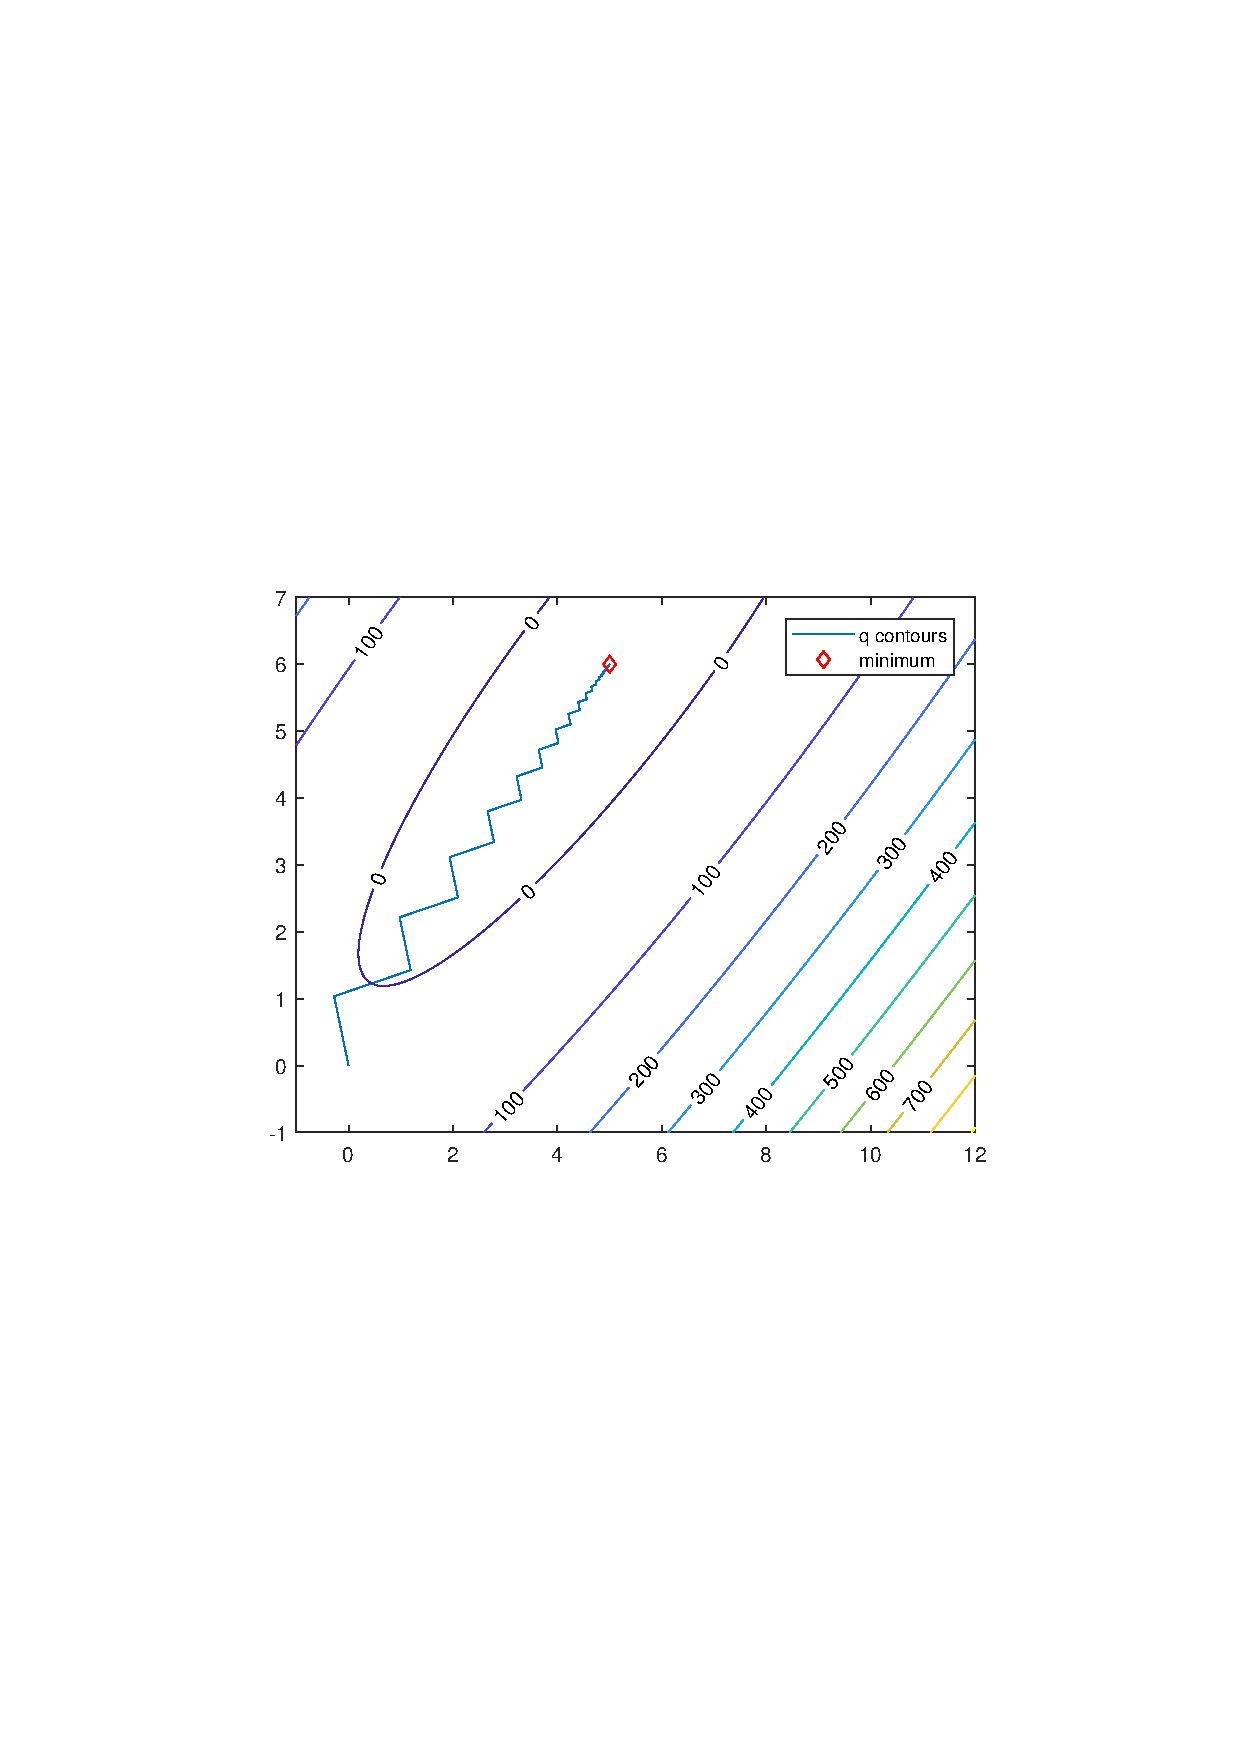
\includegraphics[width=5.7cm]{fig/1_1a.pdf}}
\subfigure{
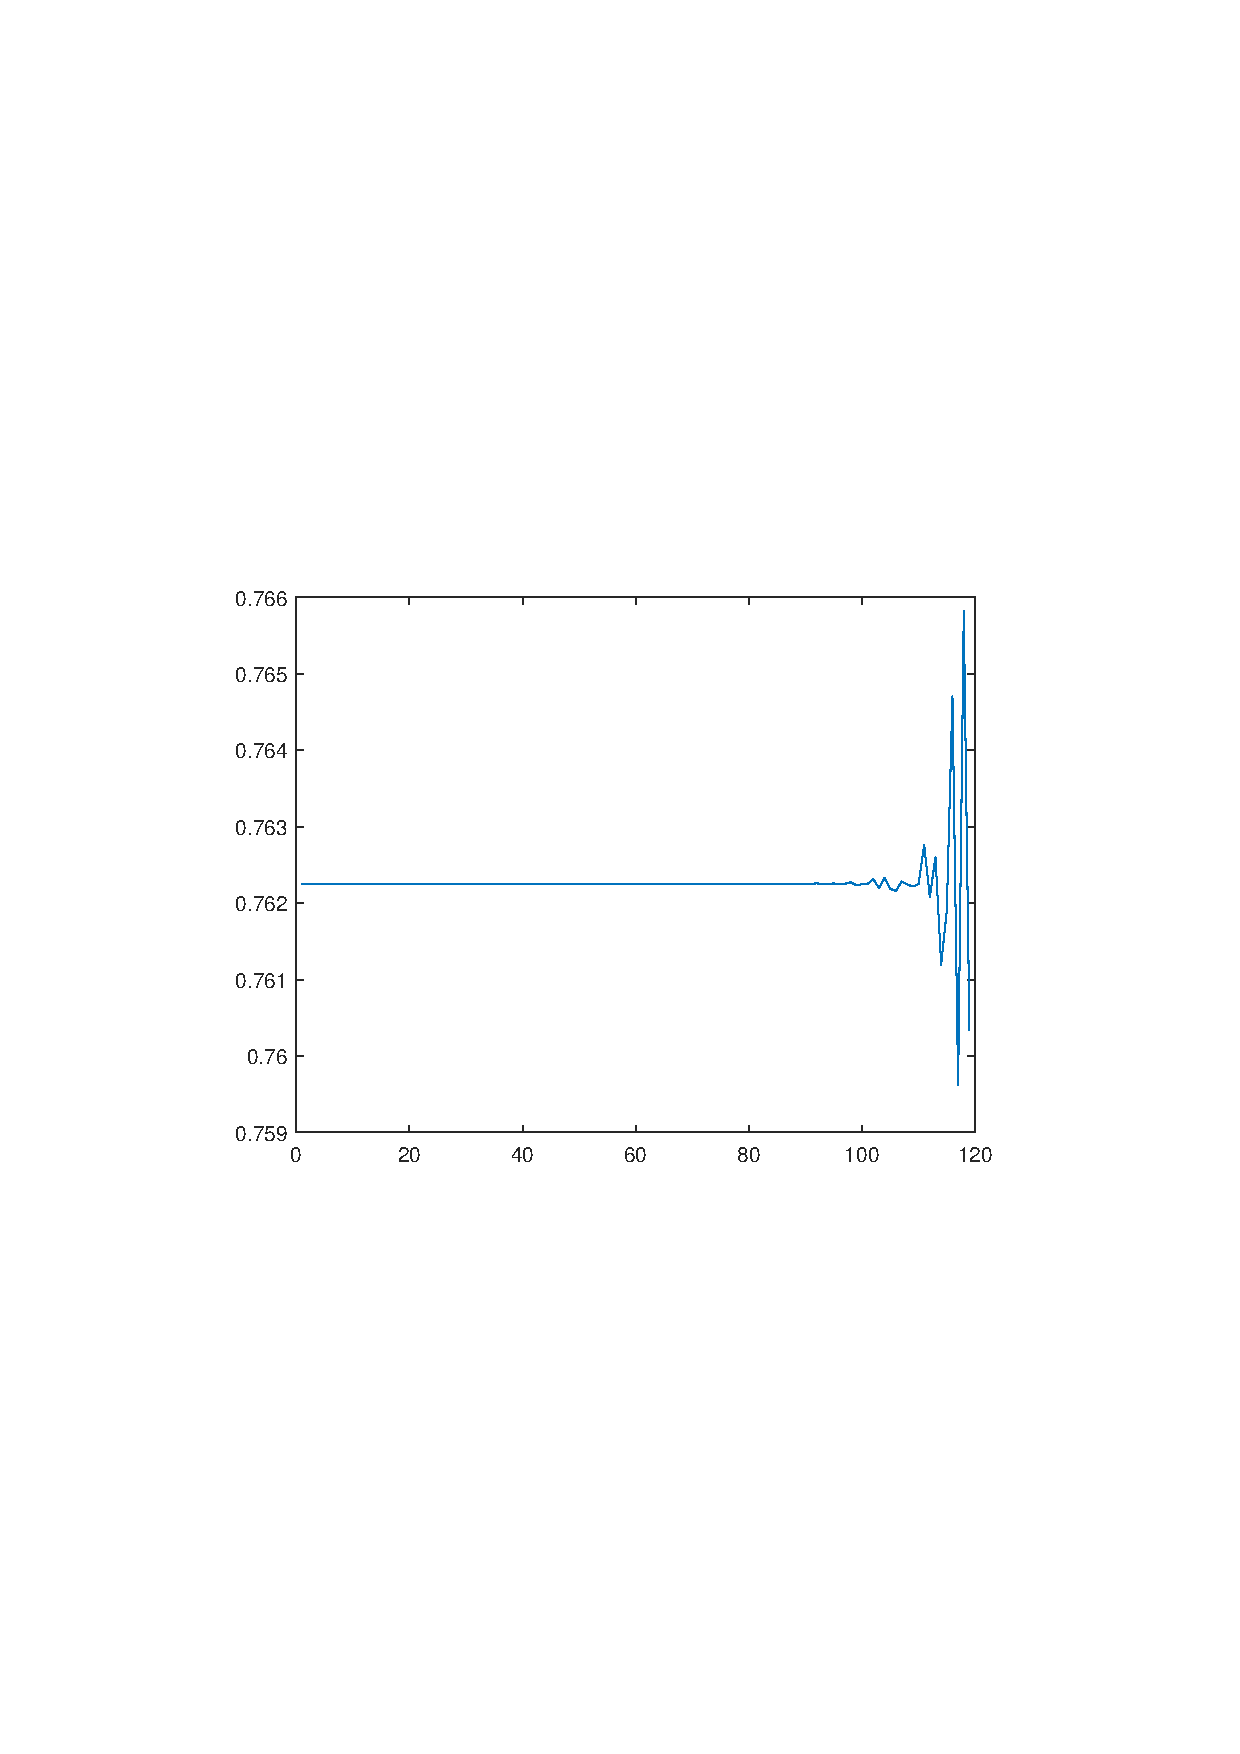
\includegraphics[width=6cm]{fig/1_1b.pdf}}
\caption{Steepest-denscent in (0,0)}
\label{Fig.lable}
\end{figure}

\begin{figure}[H]
\centering
\subfigure{
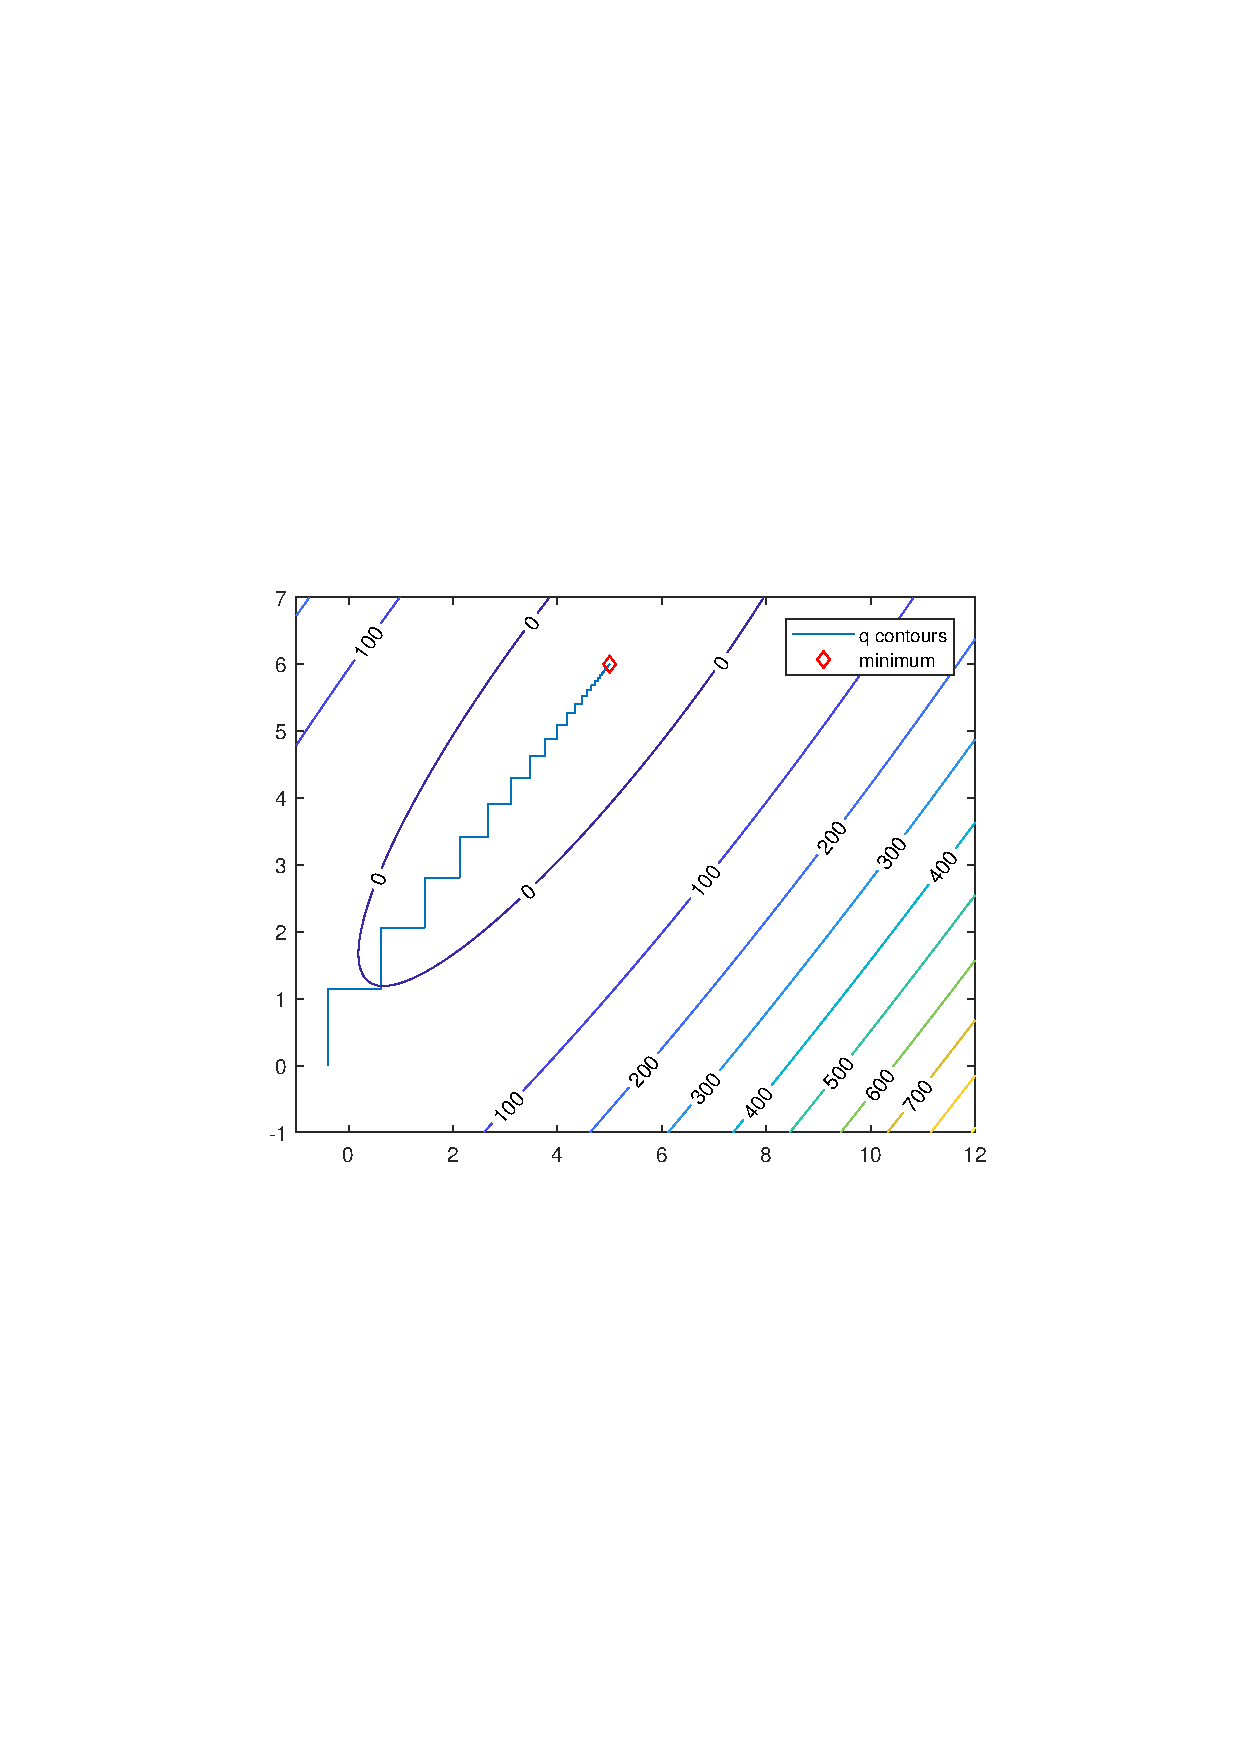
\includegraphics[width=5.7cm]{fig/1_2a.pdf}}
\subfigure{
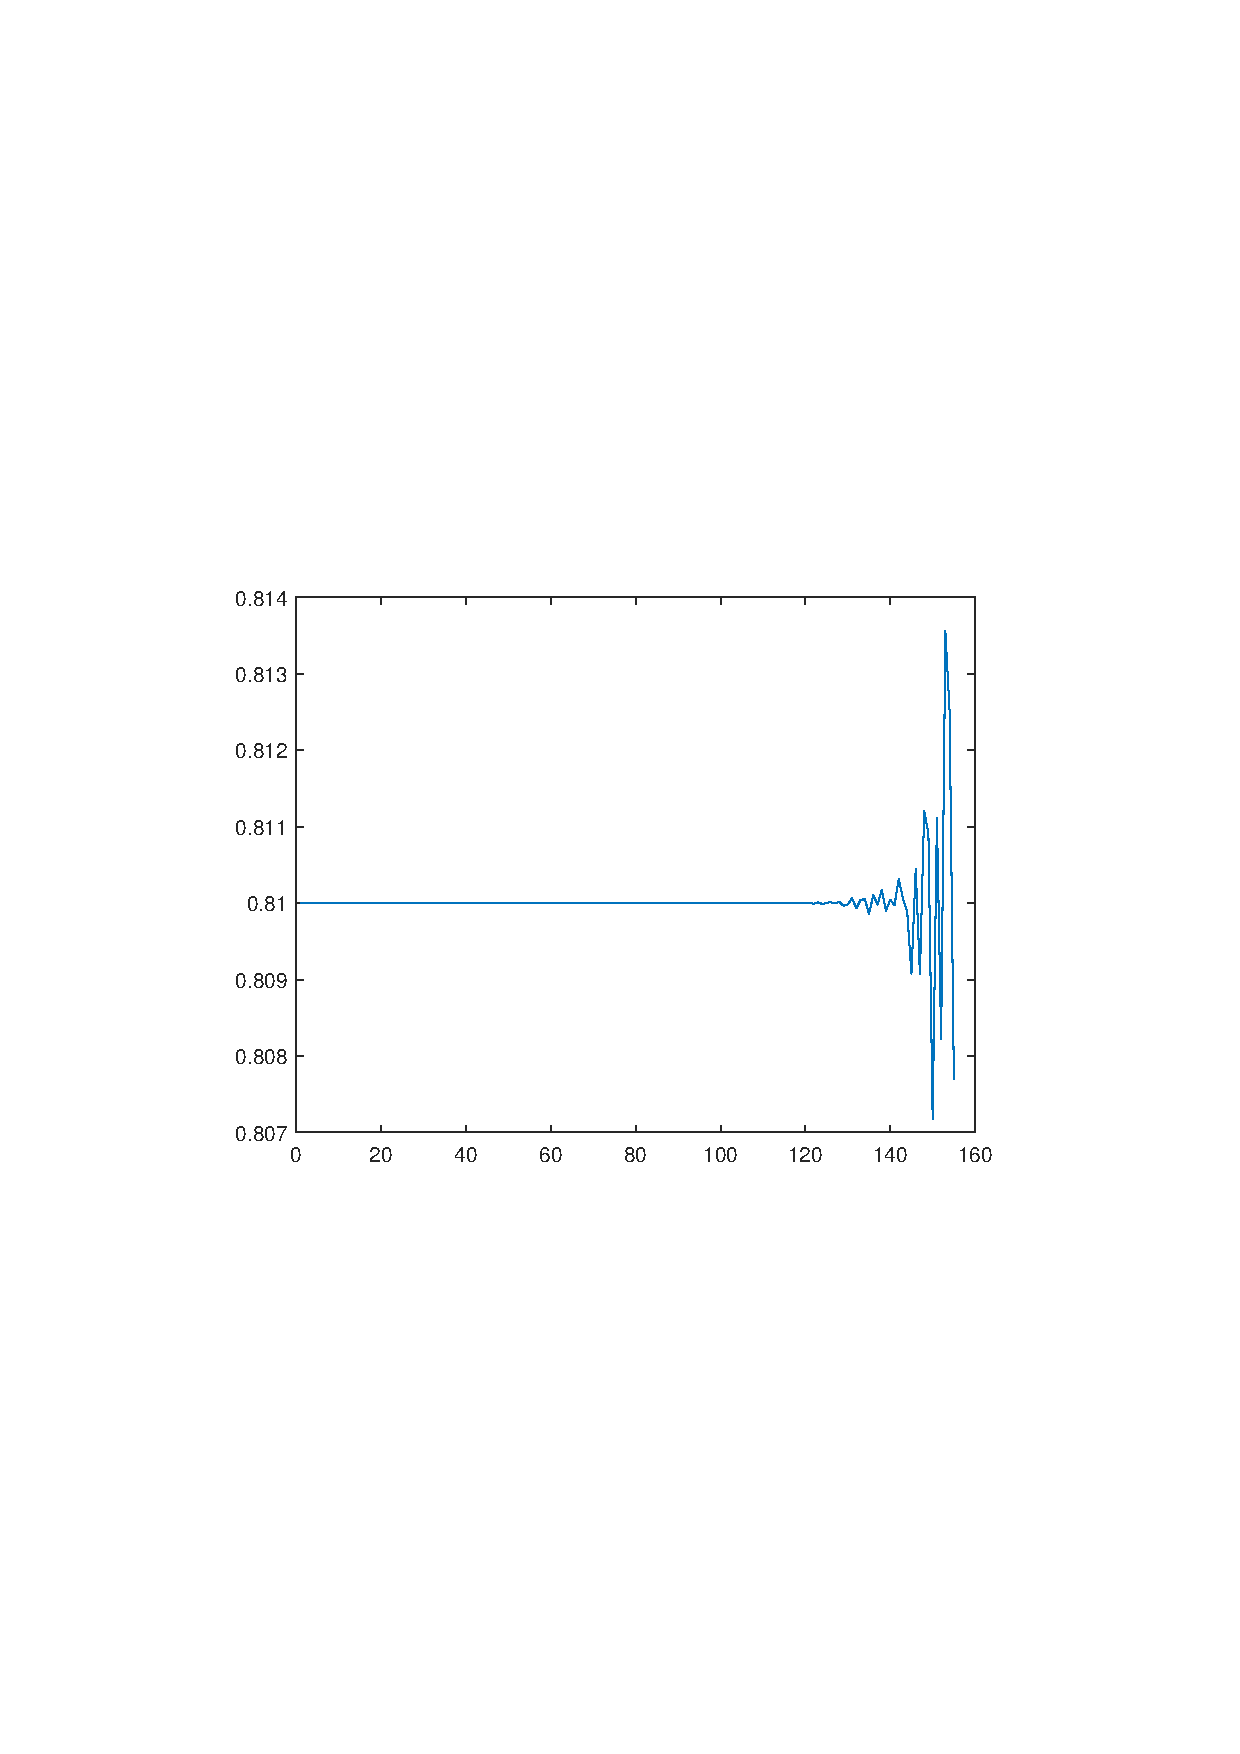
\includegraphics[width=6cm]{fig/1_2b.pdf}}
\caption{Steepest-denscent in (-0.4,0)}
\label{Fig.lable}
\end{figure}

\begin{figure}[H]
\centering
\subfigure{
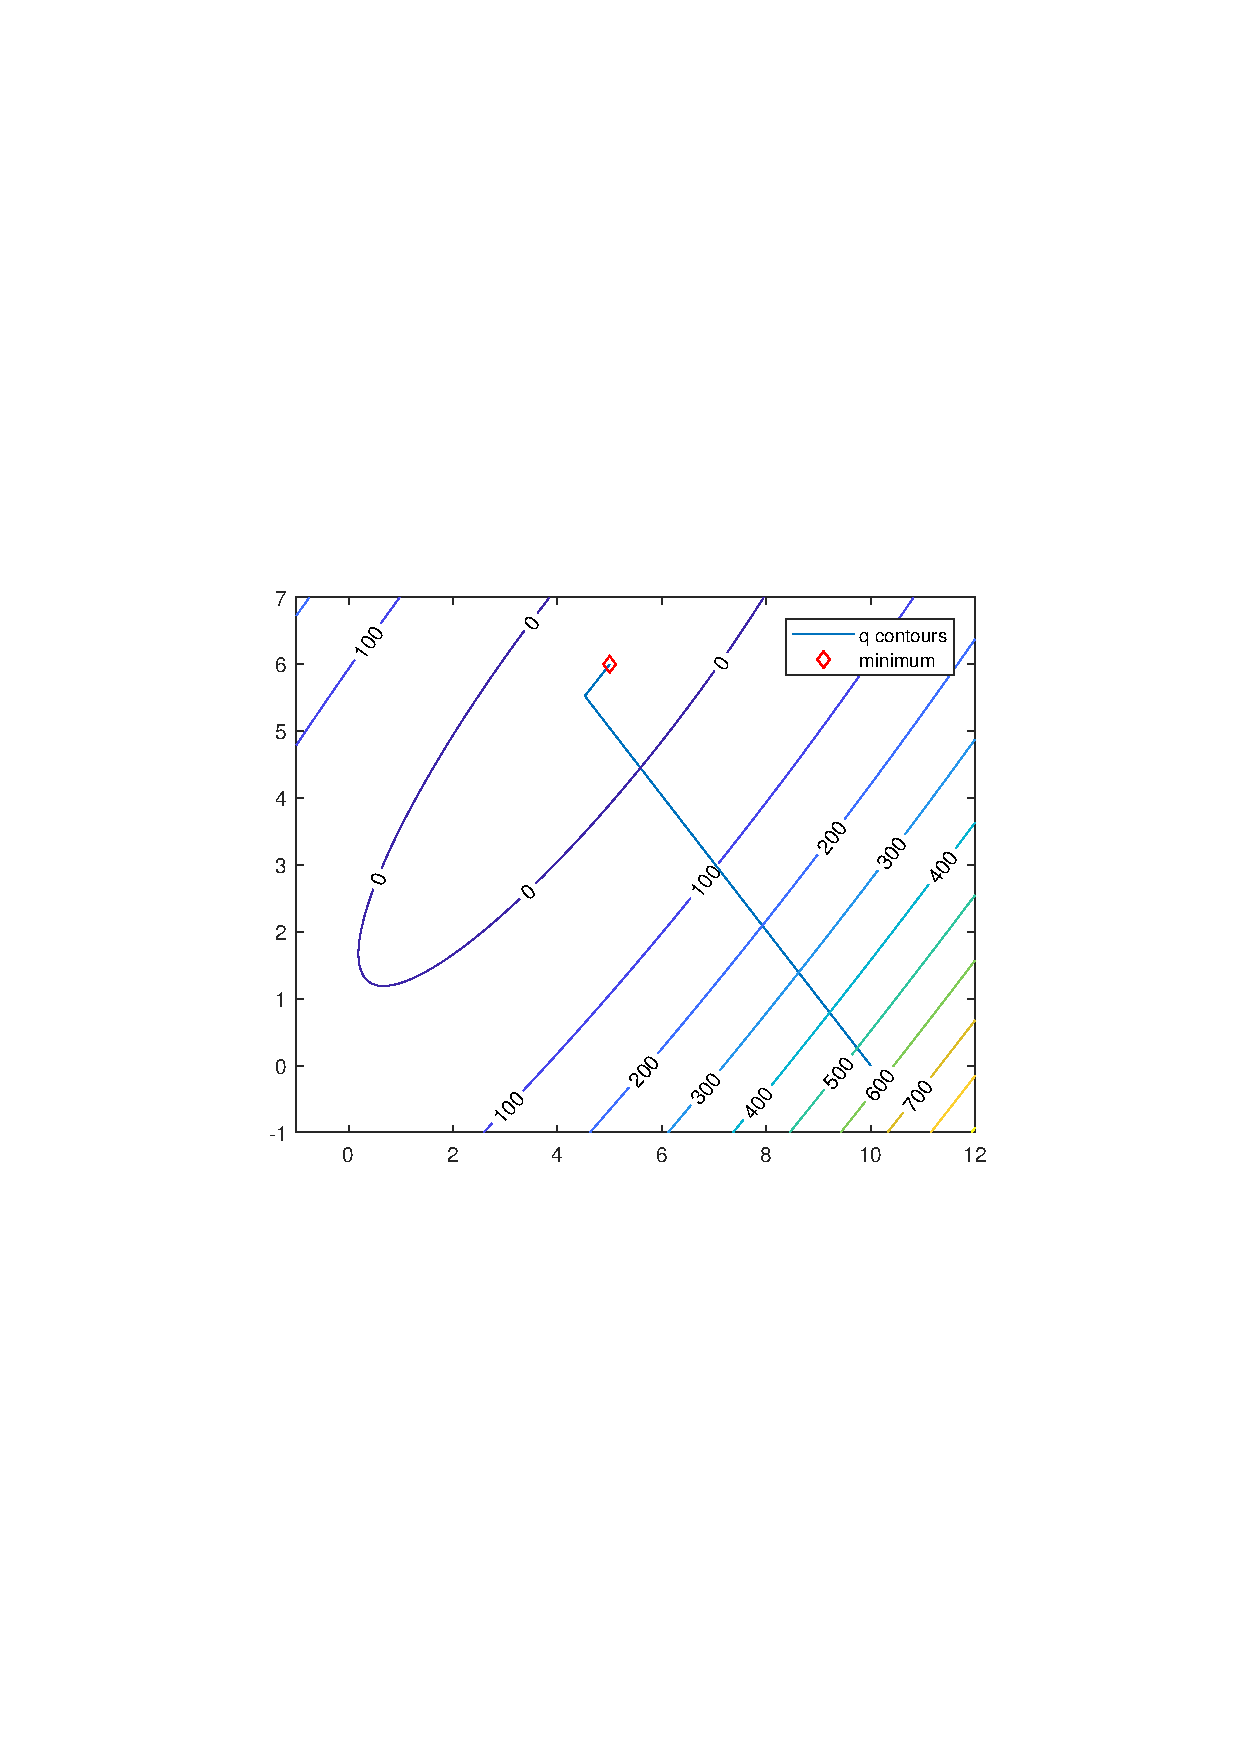
\includegraphics[width=5.7cm]{fig/1_3a.pdf}}
\subfigure{
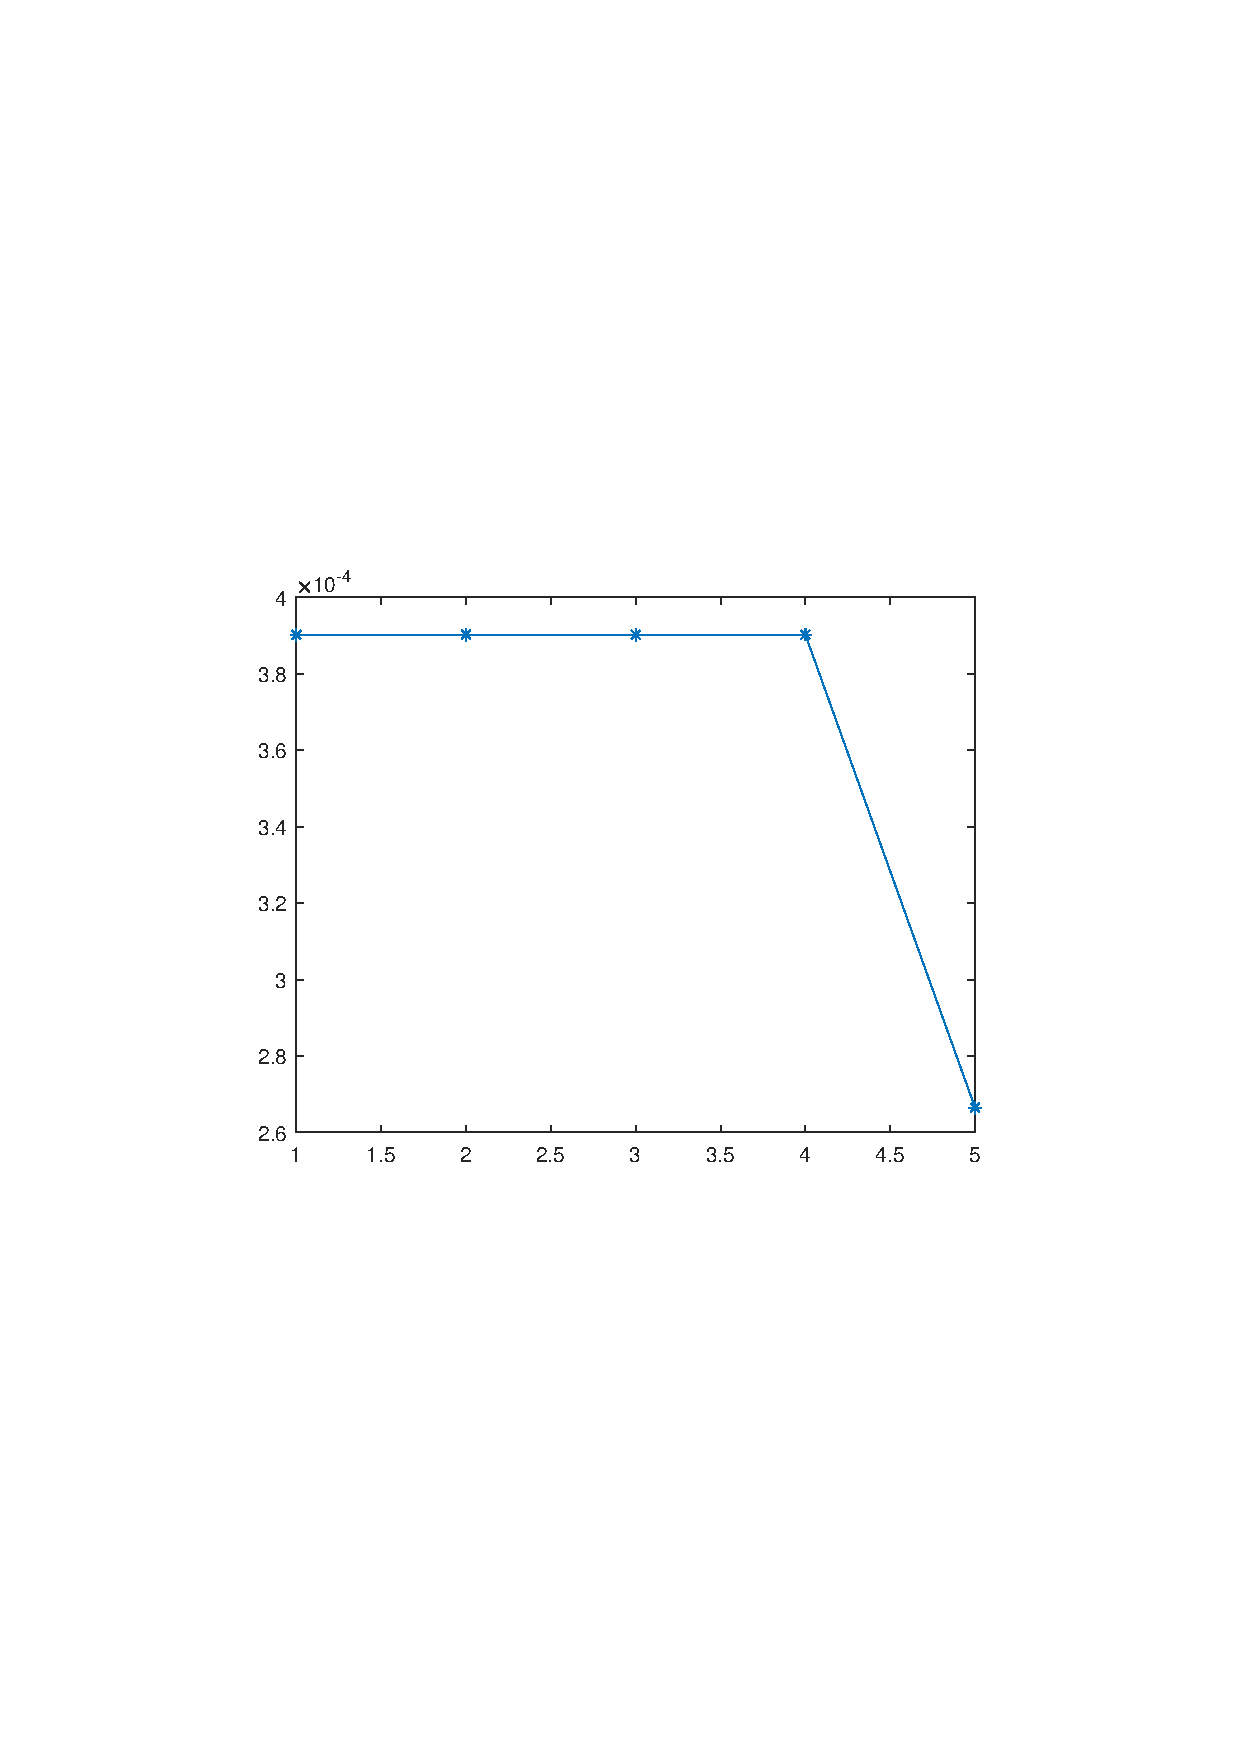
\includegraphics[width=5.8cm]{fig/1_3b.pdf}}
\caption{Steepest-denscent in (10,0)}
\label{Fig.lable}
\end{figure}

\begin{figure}[H]
\centering
\subfigure{
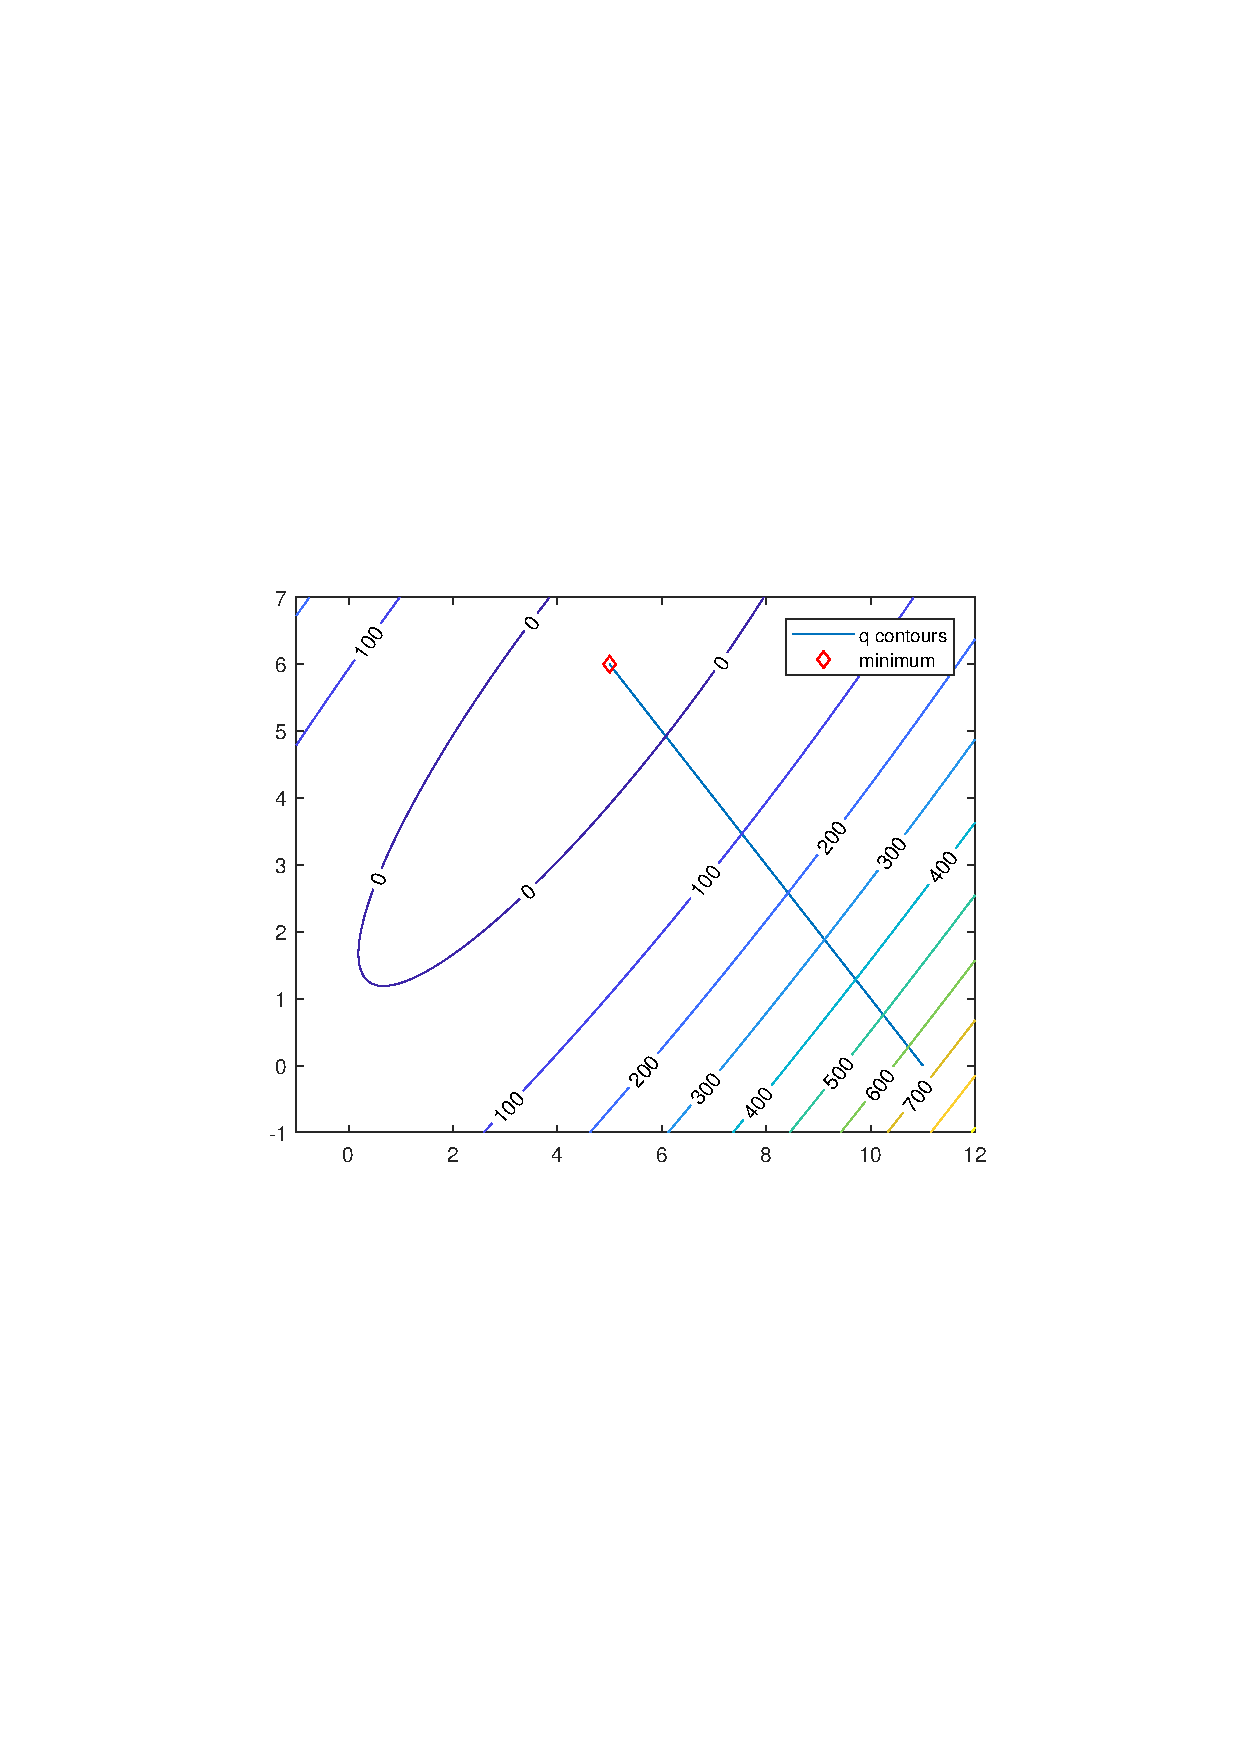
\includegraphics[width=5.8cm]{fig/1_4a.pdf}}
\subfigure{
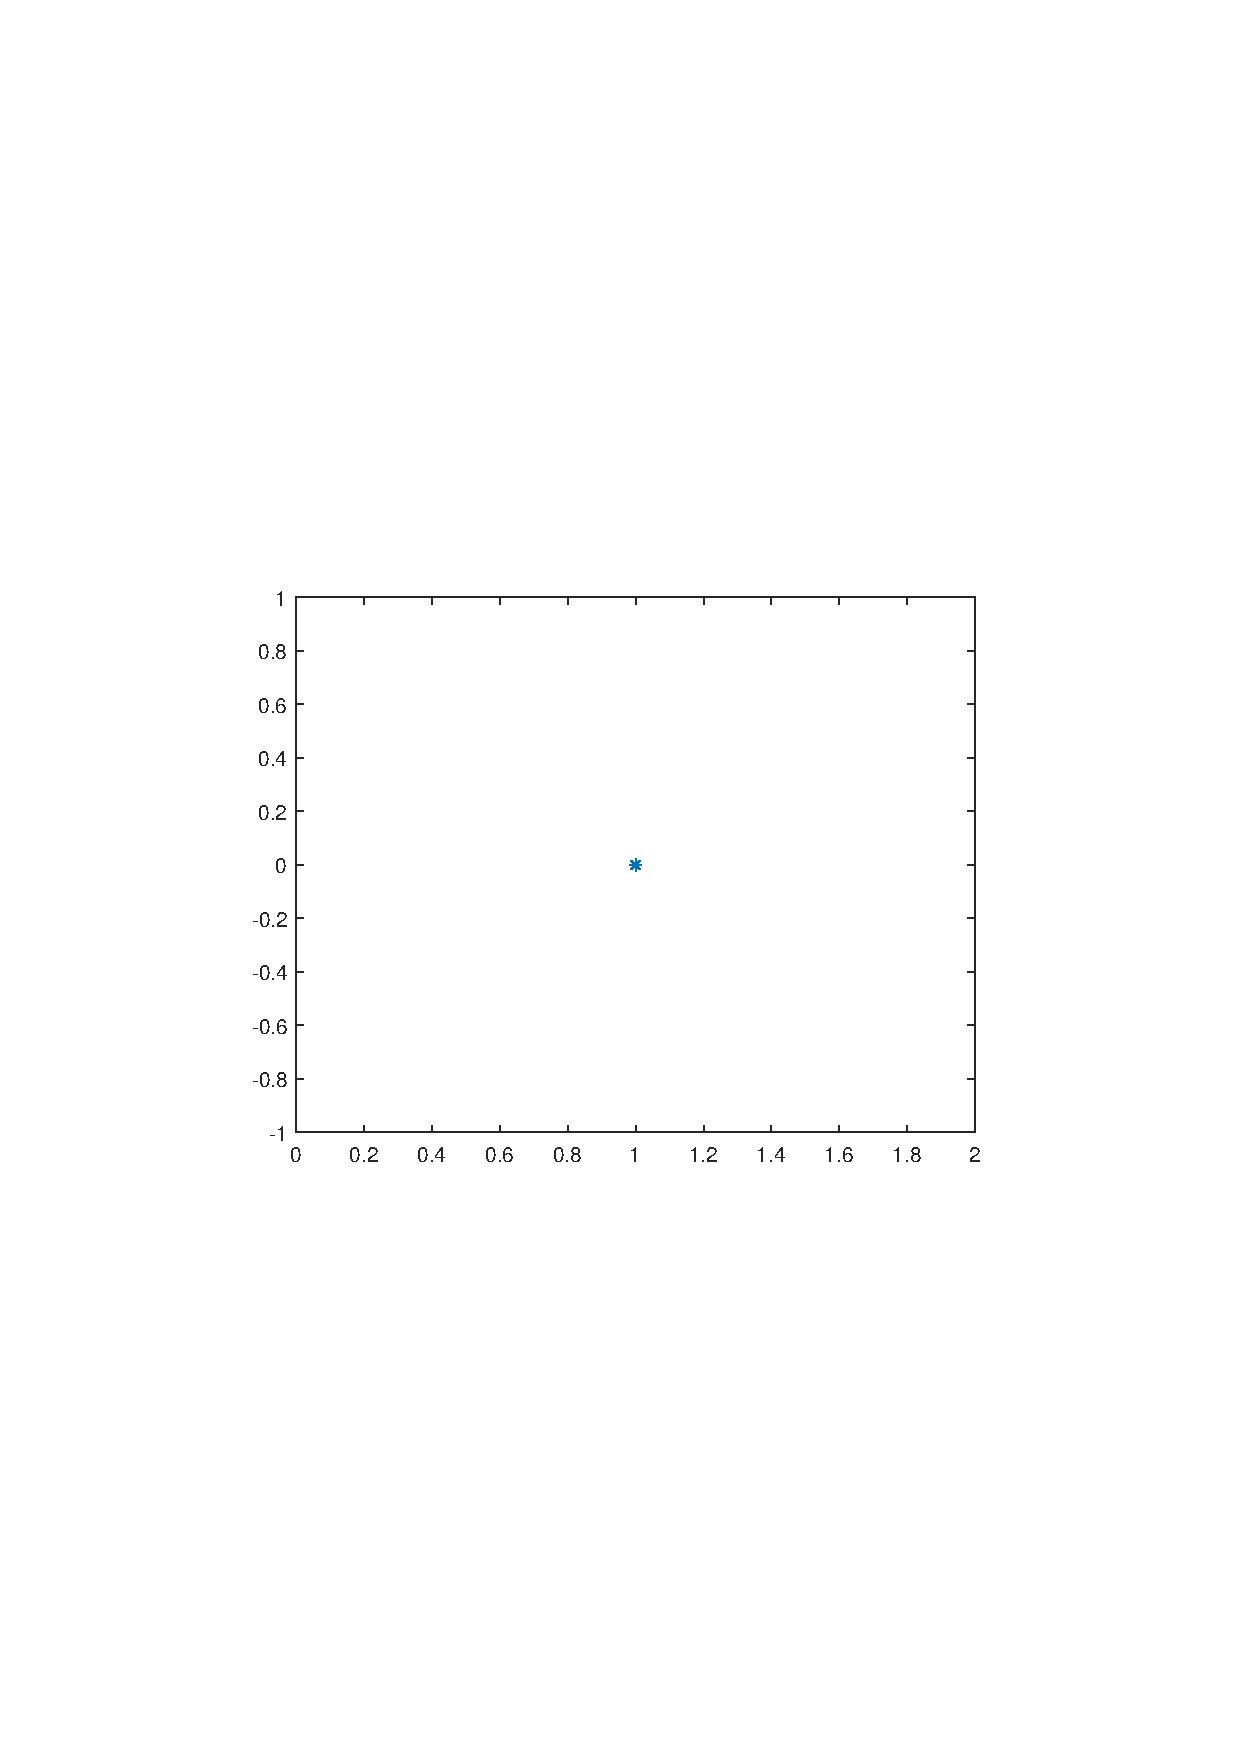
\includegraphics[width=5.9cm]{fig/1_4b.pdf}}

\caption{Steepest-denscent in (11,0)}
\label{Fig.lable}
\end{figure}

\begin{table}[H]
\centering
\caption{收敛因子比较}
	\begin{tabular}{ccccc}
	\toprule
	{起始点}&$(0,0)$&$(-0.4,0)$&$(10,0)$&$(11,0)$\\
	\midrule
	{收敛因子}&0.762255&0.810000&0.000390&0\\
	\bottomrule
	\end{tabular}
\end{table}

\subsection{分析}
由于目标函数为凸函数,故使用梯度下降法从这四个不同的起始点出发都能收敛到全局最优点,然而线性收敛因子却互不相同.

由图像可知:在迭代开始后,函数值的收敛速度稳定在一个值左右,直到接近最优点时,收敛速度开始较大幅度波动。

而且,可以看出,初始点越接近等值线椭圆的狭长端,线性收敛因子越大,在点$(-0.4,0)$处甚至达到了线性收敛因子的上界0.81,而离狭长端越远,收敛因子越小。
这是由于梯度下降在构造搜索方向时没有充分利用到函数的二阶导数信息,在面临“峡谷”状的函数时,会反复震荡到“峡谷”的另一端,而不能直接向最优值方向前进。

容易看出,等值线椭圆的长轴端斜率为$9/10$,且$(-0.4,0)=(5,6)-0.6*(9,10)$,这说明点$(-0.4,0)$刚好处在等值线椭圆的长轴上,因此也是震荡最剧烈的地方,收敛速度达到了最坏收敛速度。
\newpage
\section{Problem 5.7}
\subsection{重要参数}
\[f(x)=9x-4\ln(x-7)\]
\[g(x)=f'(x)=9-\dfrac{4}{x-7}\]
\[G(x)=g'(x)=\dfrac{4}{(x-7)^2}\]

其迭代公式为:
\begin{equation}
x^{(k+1)}=x^{(k)}-\dfrac{1}{4}(x^{(k)}-7)(9x^{(k)}-67)
\label{eq1}
\end{equation}


\subsection{算法伪代码}
\begin{algorithm}[h]  
\caption{Newton method for problem(5.7)}  
\begin{algorithmic}[1]  
\STATE Given $x^{(0)}$ and compute $g(x)=f'(x)$
\STATE Compute $G(x)=g'(x)$
\STATE Set $g^{(0)}=g(x^{(0)}),k=0$
\WHILE {$|g^{(k)}|>\epsilon$}
\STATE Set $s^{(k)}=-g^{(k)}/G^{(k)}$
\STATE Set $x^{(k+1)}=x^{(k)}+s^{(k)}$
\STATE Set $k=k+1$
\ENDWHILE
\end{algorithmic}  
\end{algorithm}  



\subsection{计算结果展示}
% Table generated by Excel2LaTeX from sheet 'Sheet1'
\begin{table}[htbp]
  \centering
  \caption{迭代5次过程}
    \begin{tabular}{clllll}
\toprule
  $x^{(0)}$&7.4  & 7.2  & 7.01 &7.80  & 7.88 \\
	\midrule
   $x^{(1)}$& 7.44  & 7.31  & 7.019775 & 7.16  & 7.0176 \\
    $x^{(2)}$&7.4444 & 7.403775 & 7.038670136 & 7.2624 & 7.03450304 \\
    $x^{(3)}$&7.44444444 & 7.440722936 & 7.073975668 & 7.36987904 & 7.066327546 \\
   $ x^{(4)}$&7.444444444 & 7.444413283 & 7.135638438 & 7.431934445 & 7.122756569 \\
    $x^{(5)}$&7.444444444 & 7.444444442 & 7.229881858 & 7.444092319 & 7.211607493 \\
	\midrule
    $f(x^{(5)})$&70.24372086 & 70.24372086 & 70.94969577 & 70.24372212 & 71.11655611 \\
	\bottomrule
    \end{tabular}%
  \label{tab:addlabel}%
\end{table}%

% Table generated by Excel2LaTeX from sheet 'Sheet1'
\begin{table}[htbp]
  \centering
  \caption{大范围迭代结果}
    \begin{tabular}{|c|c|c|c|}
    \hline
    初始点   & 迭代终止点 & 初始点   & 迭代终止点 \\
    \hline
    5     & -Inf  & 9     & -Inf \\
    \hline
    5.25  & -Inf  & 9.25  & -Inf \\
    \hline
    5.5   & -Inf  & 9.5   & -Inf \\
    \hline
    5.75  & -Inf  & 9.75  & -Inf \\
    \hline
    6     & -Inf  & 10    & -Inf \\
    \hline
    6.25  & -Inf  & 10.25 & -Inf \\
    \hline
    6.5   & -Inf  & 10.5  & -Inf \\
    \hline
    6.75  & -Inf  & 10.75 & -Inf \\
    \hline
    7     & 7     & 11    & -Inf \\
    \hline
    7.25  & 7.44444444444445 & 11.25 & -Inf \\
    \hline
    7.5   & 7.44444444444445 & 11.5  & -Inf \\
    \hline
    7.75  & 7.44444444444445 & 11.75 & -Inf \\
    \hline
    8     & -Inf  & 12    & -Inf \\
    \hline
    8.25  & -Inf  & 12.25 & -Inf \\
    \hline
    8.5   & -Inf  & 12.5  & -Inf \\
    \hline
    8.75  & -Inf  & 12.75 & -Inf \\
    \hline
    \end{tabular}%
  \label{tab:addlabel}%
\end{table}%


由MATLAB函数fminsearch求得最优解为:\[x^{\star}=7.444421386718750,\quad f(x^{\star})=70.243720870248540\]


\subsection{收敛域内点的迭代情况}
\begin{figure}[H]
\centering
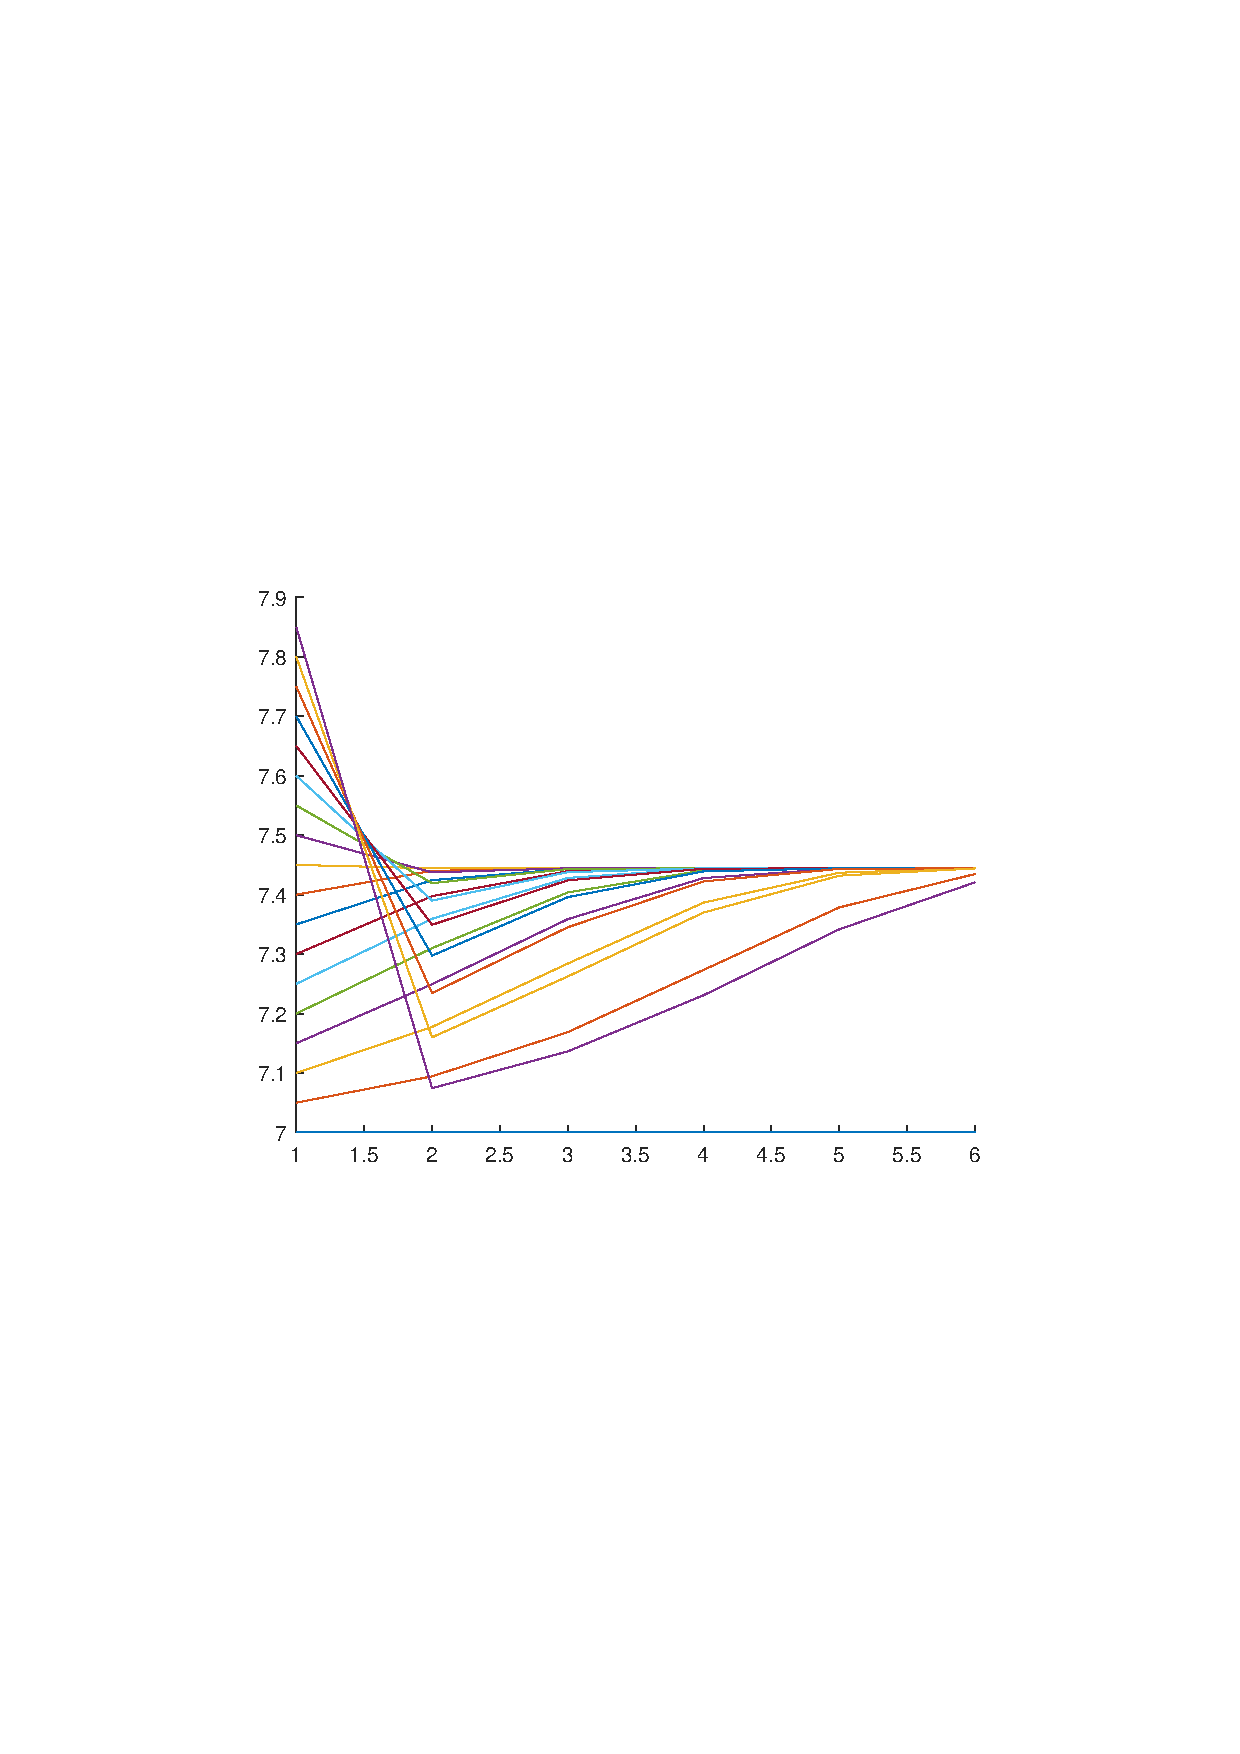
\includegraphics[width=10cm]{fig/2_1.pdf}
\end{figure}

\begin{figure}[H]
\centering
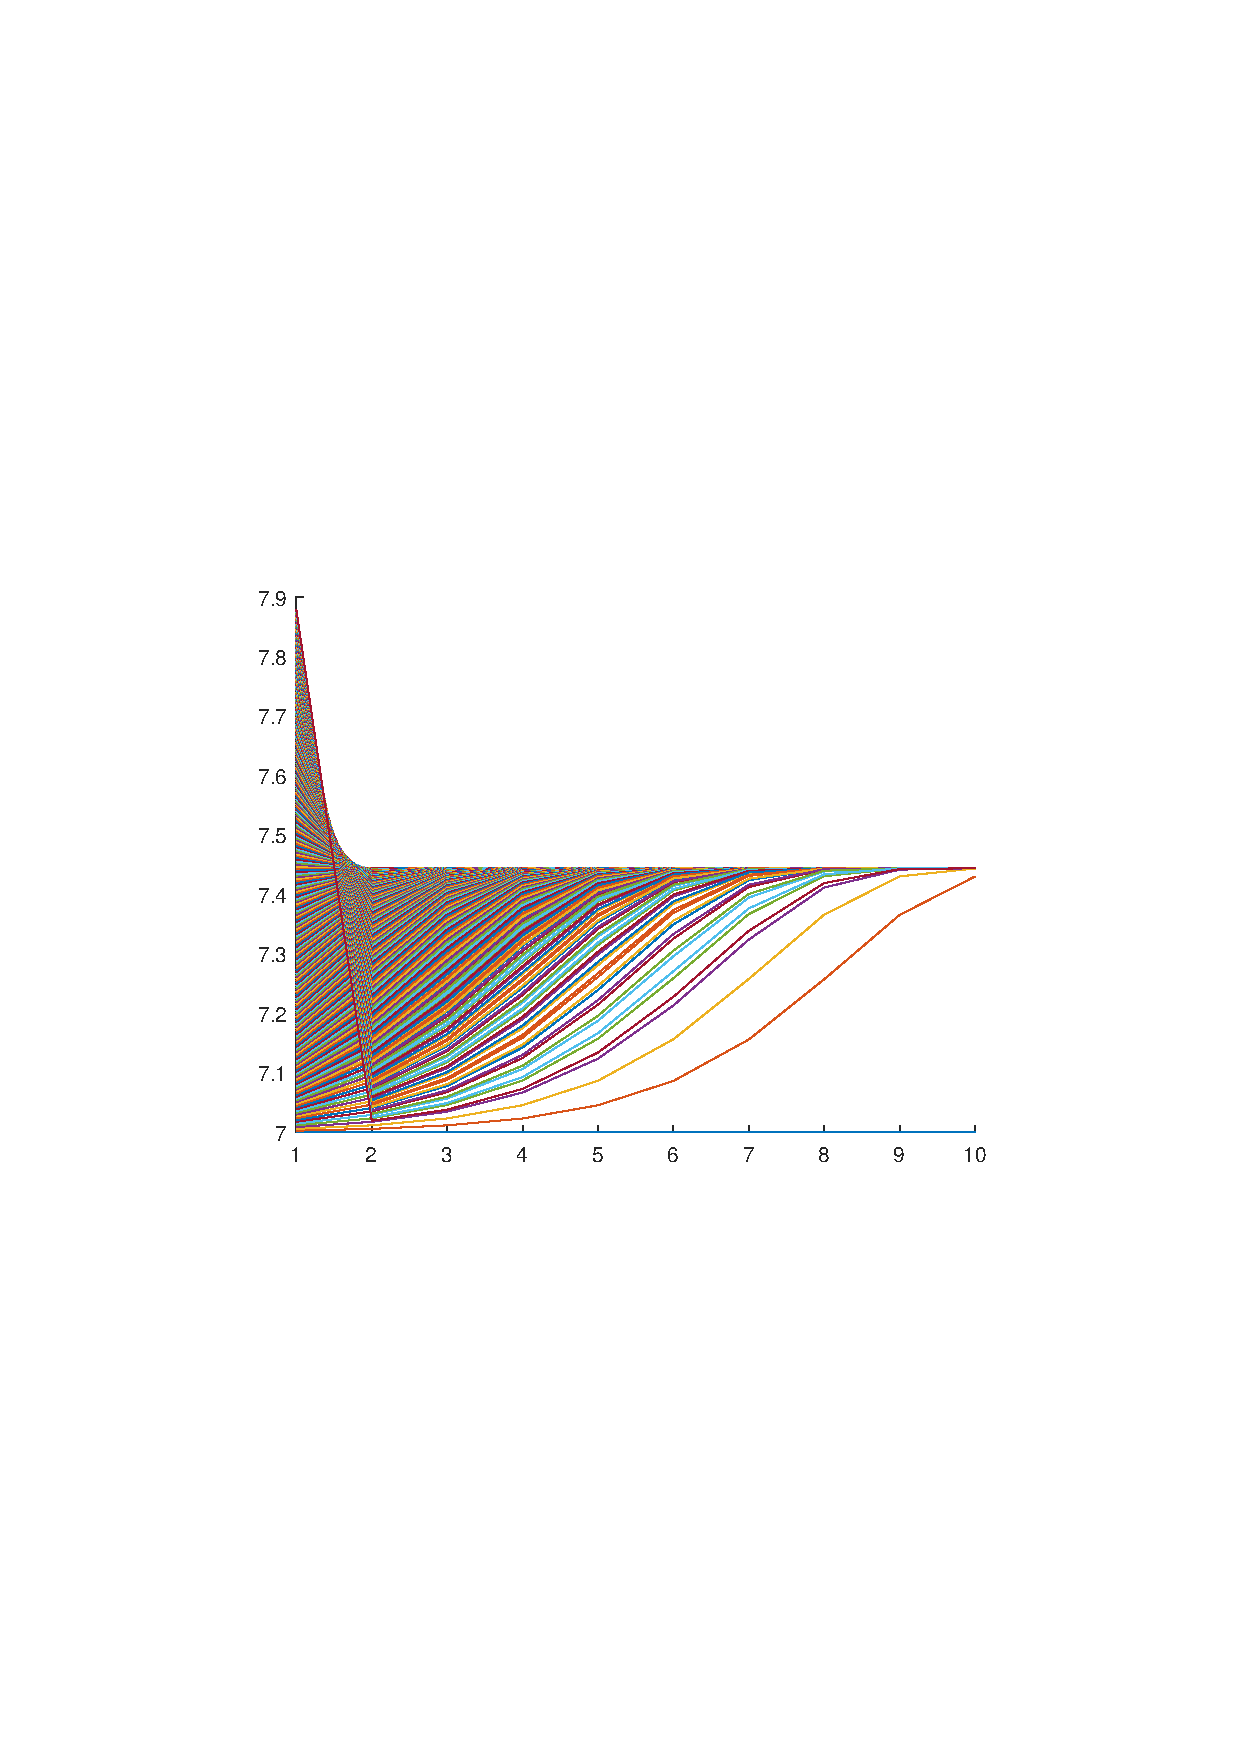
\includegraphics[width=10cm]{fig/2_2.pdf}
\end{figure}

\begin{figure}[H]
\centering
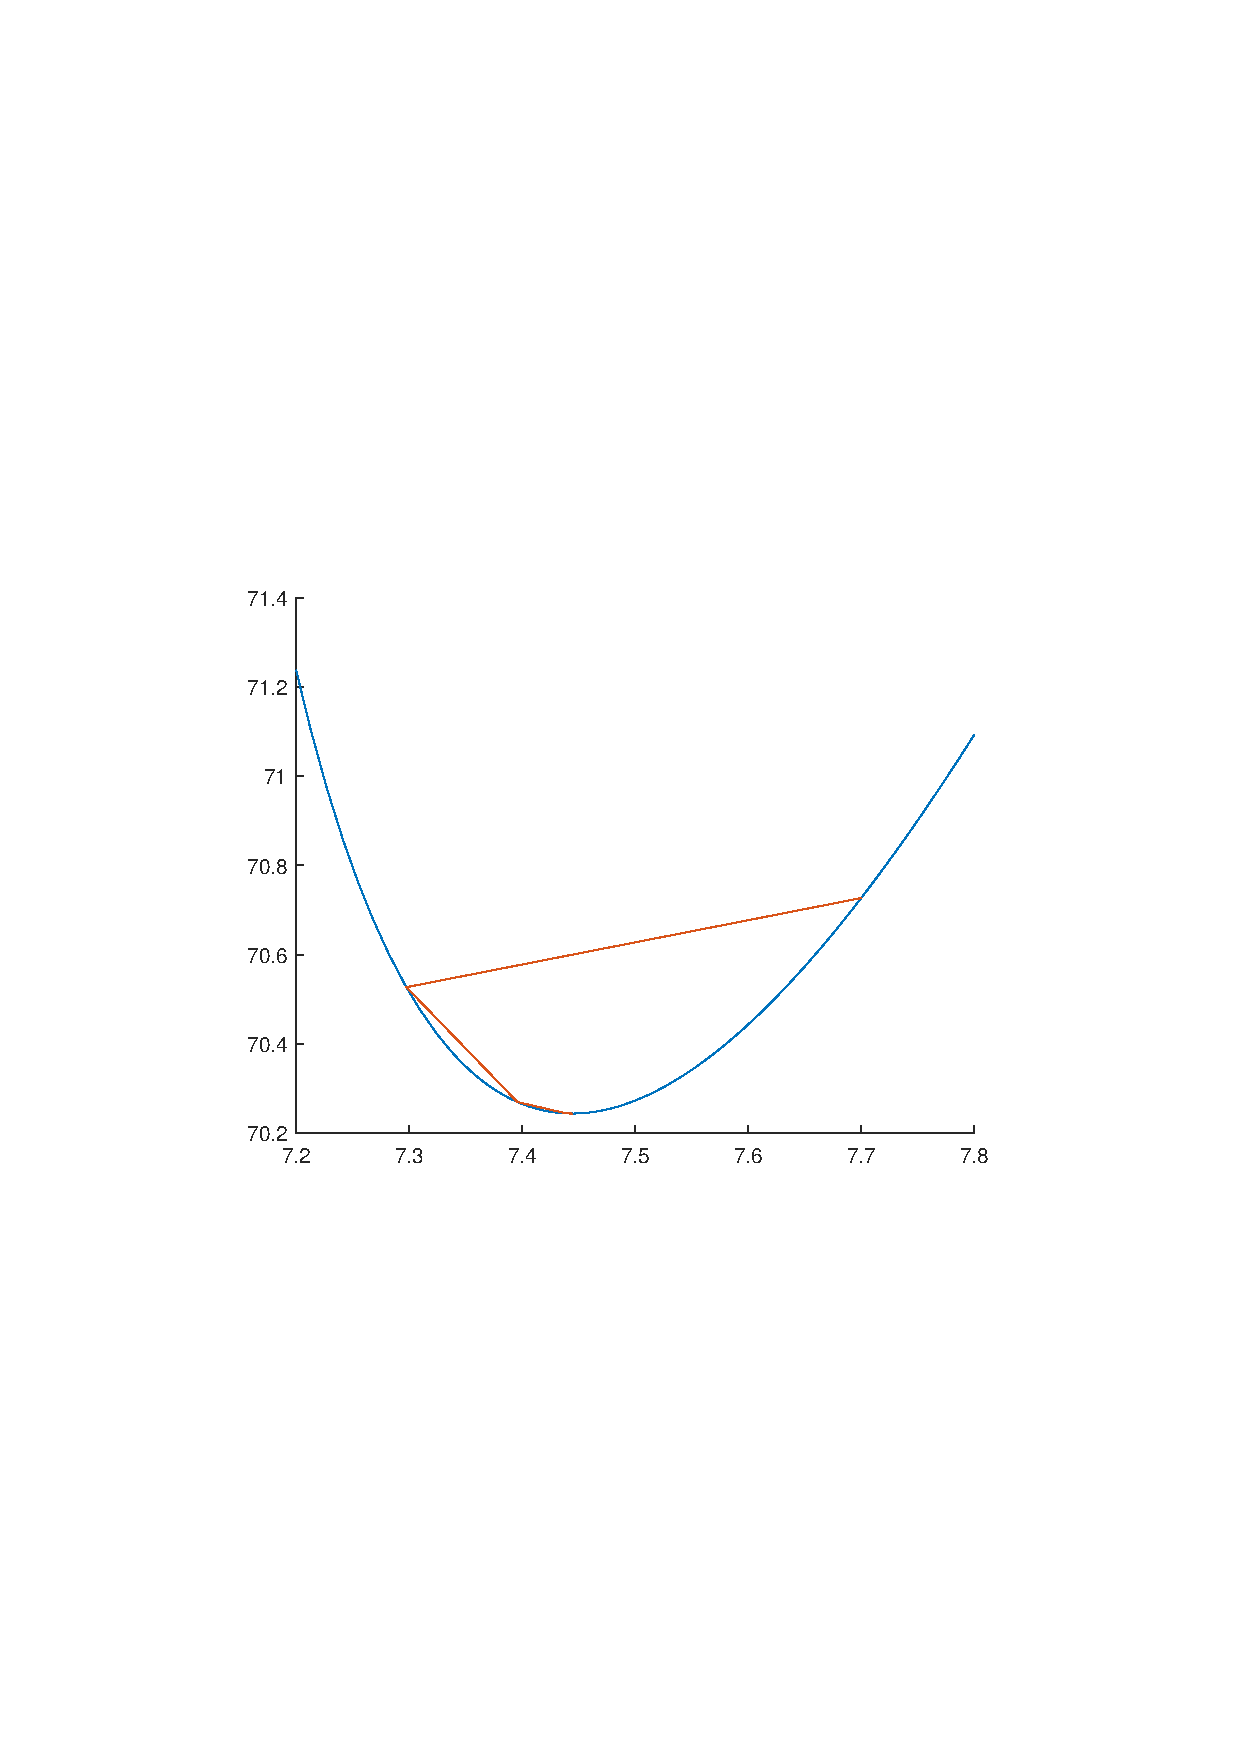
\includegraphics[width=11cm]{fig/2_3.pdf}
\end{figure}

%\newpage
\subsection{总结分析}
\subsection*{关于收敛域的分析}

首先由于$G(x)>0$,故在定义域内总能收敛。

然后我们观察迭代公式(equation:\ref{eq1})
\[x^{(k+1)}=x^{(k)}-\dfrac{1}{4}(x^{(k)}-7)(9x^{(k)}-67)\]
可以得出以下结论:
\begin{itemize}
\item
容易看出两个稳定点为$x'=7\ and\ x^{\star}=67/9$
\item
若初始点在定义域内,则要求$x_0>=7$
\item
然后要避免$x_k$迭代时使得$x^{(k+1)}$跳出定义域,
因此解方程
\[7=x^{(k)}-\dfrac{1}{4}(x^{(k)}-7)(9x^{(k)}-67)\]

得到解:$x_k=7\ or \ 71/9$
\item
因此该迭代公式的收敛域为$(7,71/9)$
\end{itemize}

\subsection*{点的迭代性质分析}
观察点的迭代图像可以看到:
\begin{itemize}
\item
在收敛域$(7,71/9)$内$x$将逐渐收敛到稳定点$x^{\star}=67/9$
\item
若起始点$x_0\in (67/9,71/9)$,则其迭代第一步的步长非常大,使得一下子就跃到$67/9$以下,然后慢慢朝稳定点方向靠近,而且一开始离稳定点越大,步长越大,这可由公式(equation:\ref{eq1})解释

\item
但当$x_0$离稳定点太远,超出$71/9$时,将会使得下一步迭代步长过大,导致超出定义域。

\item
若起始点$x_0\in (7,67/9)$时,$x_0$不会像之前那样猛烈地向稳定点$x^{\star}$迈进,而是缓慢地迭代,而越远离稳定点$x^{\star}$,迭代得越慢

\item
透过公式(equation:\ref{eq1}),我们可以用一种形象的语言来描述这种现象:当$x_0>67/9$时,它受到了两个稳定点$x',x^{\star}$的“吸引”,因此迈出的步长特别大。而当$7<x_0<67/9$时,$x^{\star}$对它的“吸引力”被另一个稳定点$x'$的“吸引力”抵消了一部分,而离$x'$越近,“引力”被抵消得越厉害,迭代也就越慢.
\end{itemize}








\newpage
\section{Problem 5.8}
\subsection{重要参数}
\begin{align}
f({x_1},{x_2})=&-9{x_1}-10{x_2}\nonumber\\
&-\mu \big[\ln(-{x_1}-{x_2}+100)+\ln (-{x_1}+{x_2}+50)+\ln ({x_1})+\ln ({x_2})\big]
\nonumber
\end{align}


\begin{align}
\bm{g}(x_1, x_2) &= \nabla f(x_1, x_2)\nonumber\\
&=
\begin{bmatrix}
-9 -\dfrac{\mu}{x_1 }+\dfrac{\mu}{100 - x_1 - x_2} + \dfrac{\mu}{50 - x_1 + x_2} \nonumber\\
-10 - \dfrac{\mu}{x_2 }+\dfrac{\mu}{100 - x_1 - x_2} - \dfrac{\mu}{50 - x_1 + x_2}
\end{bmatrix}\nonumber\\\nonumber
\end{align}
\begin{align}
&\bm{G}[x_1, x_2] \nonumber\\
=& \nabla \bm{g}(x_1, x_2)\nonumber \\
=&
\begin{bmatrix}
\dfrac{1}{{x_1}^2 }+\dfrac{1}{(100 - x_1 - x_2)^2} + \dfrac{1}{(50 - x_1 + x_2)^2} 
&\dfrac{1}{(100 - x_1 - x_2)^2} - \dfrac{1}{(50 - x_1 + x_2)^2}\\
\dfrac{1}{(100 - x_1 - x_2)^2} - \dfrac{1}{(50 - x_1 + x_2)^2}&
\dfrac{1}{{x_2}^2 }+\dfrac{1}{(100 - x_1 - x_2)^2} + \dfrac{1}{(50 - x_1 + x_2)^2} 
\end{bmatrix}\nonumber\\ \nonumber
\end{align}

\subsection{算法伪代码}
\begin{algorithm}[h]  
\caption{Backtracking-Armijo Line Search} 
\label{Amj} 
\begin{algorithmic}[1]  
\STATE Choose $\bar{\alpha}>0,\quad \gamma,\rho\in (0,1)$
\STATE Set $\alpha=\bar{\alpha}$
\WHILE {$\phi(\alpha)>\phi(0)+\rho\phi'(0)\alpha$}
\STATE Set $\alpha=\gamma\alpha$
\ENDWHILE
\RETURN $\alpha$ as $\alpha_k$
\end{algorithmic}  
\end{algorithm}

\begin{algorithm}[h]  
\caption{Newton method without Armijo Line Searchfor problem(5.8)}  
\begin{algorithmic}[1]  
\STATE Given $\bm{x}^{(0)}$ and compute $\bm{g}(\bm{x})= \nabla f(\bm{x})$
\STATE Compute $\bm{G}(\bm{x})= \nabla {\bm{g}(\bm{x})}^T$
\STATE Set $\bm{g}^{(0)}=\bm{g}(\bm{x}^{(0)}),k=0$
\WHILE {$\|\bm{g}^{(k)}\|_2>\epsilon$}
\STATE Set $\bm{s}^{(k)}=-{\bm{G}^{(k)}}^{-1}\bm{g}^{(k)}$
\STATE Set $\bm{x}^{(k+1)}=\bm{x}^{(k)}+\bm{s}^{(k)}$
\STATE Set $k=k+1$
\ENDWHILE
\end{algorithmic}  
\end{algorithm} 

\begin{algorithm}[h]  
\caption{Newton method with Armijo Line Searchfor problem(5.58)}  
\label{NewtonAmj} 
\begin{algorithmic}[1]  
\STATE Given $\bm{x}^{(0)}$ and compute $\bm{g}(\bm{x})= \nabla f(\bm{x})$
\STATE Compute $\bm{G}(\bm{x})= \nabla {\bm{g}(\bm{x})}^T$
\STATE Set $\bm{g}^{(0)}=\bm{g}(\bm{x}^{(0)}),k=0$
\WHILE {$\|\bm{g}^{(k)}\|_2>\epsilon$}
\STATE Set $\bm{s}^{(k)}=-{\bm{G}^{(k)}}^{-1}\bm{g}^{(k)}$
\STATE Compute $\alpha_k$ by Line Search(\textbf{Algorithm} \ref{Amj})
\STATE Set $\bm{x}^{(k+1)}=\bm{x}^{(k)}+\alpha_k\bm{s}^{(k)}$
\STATE Set $k=k+1$
\ENDWHILE
\end{algorithmic}  
\end{algorithm} 



\subsection{迭代点运动轨迹展示}
\begin{figure}[H]
\centering
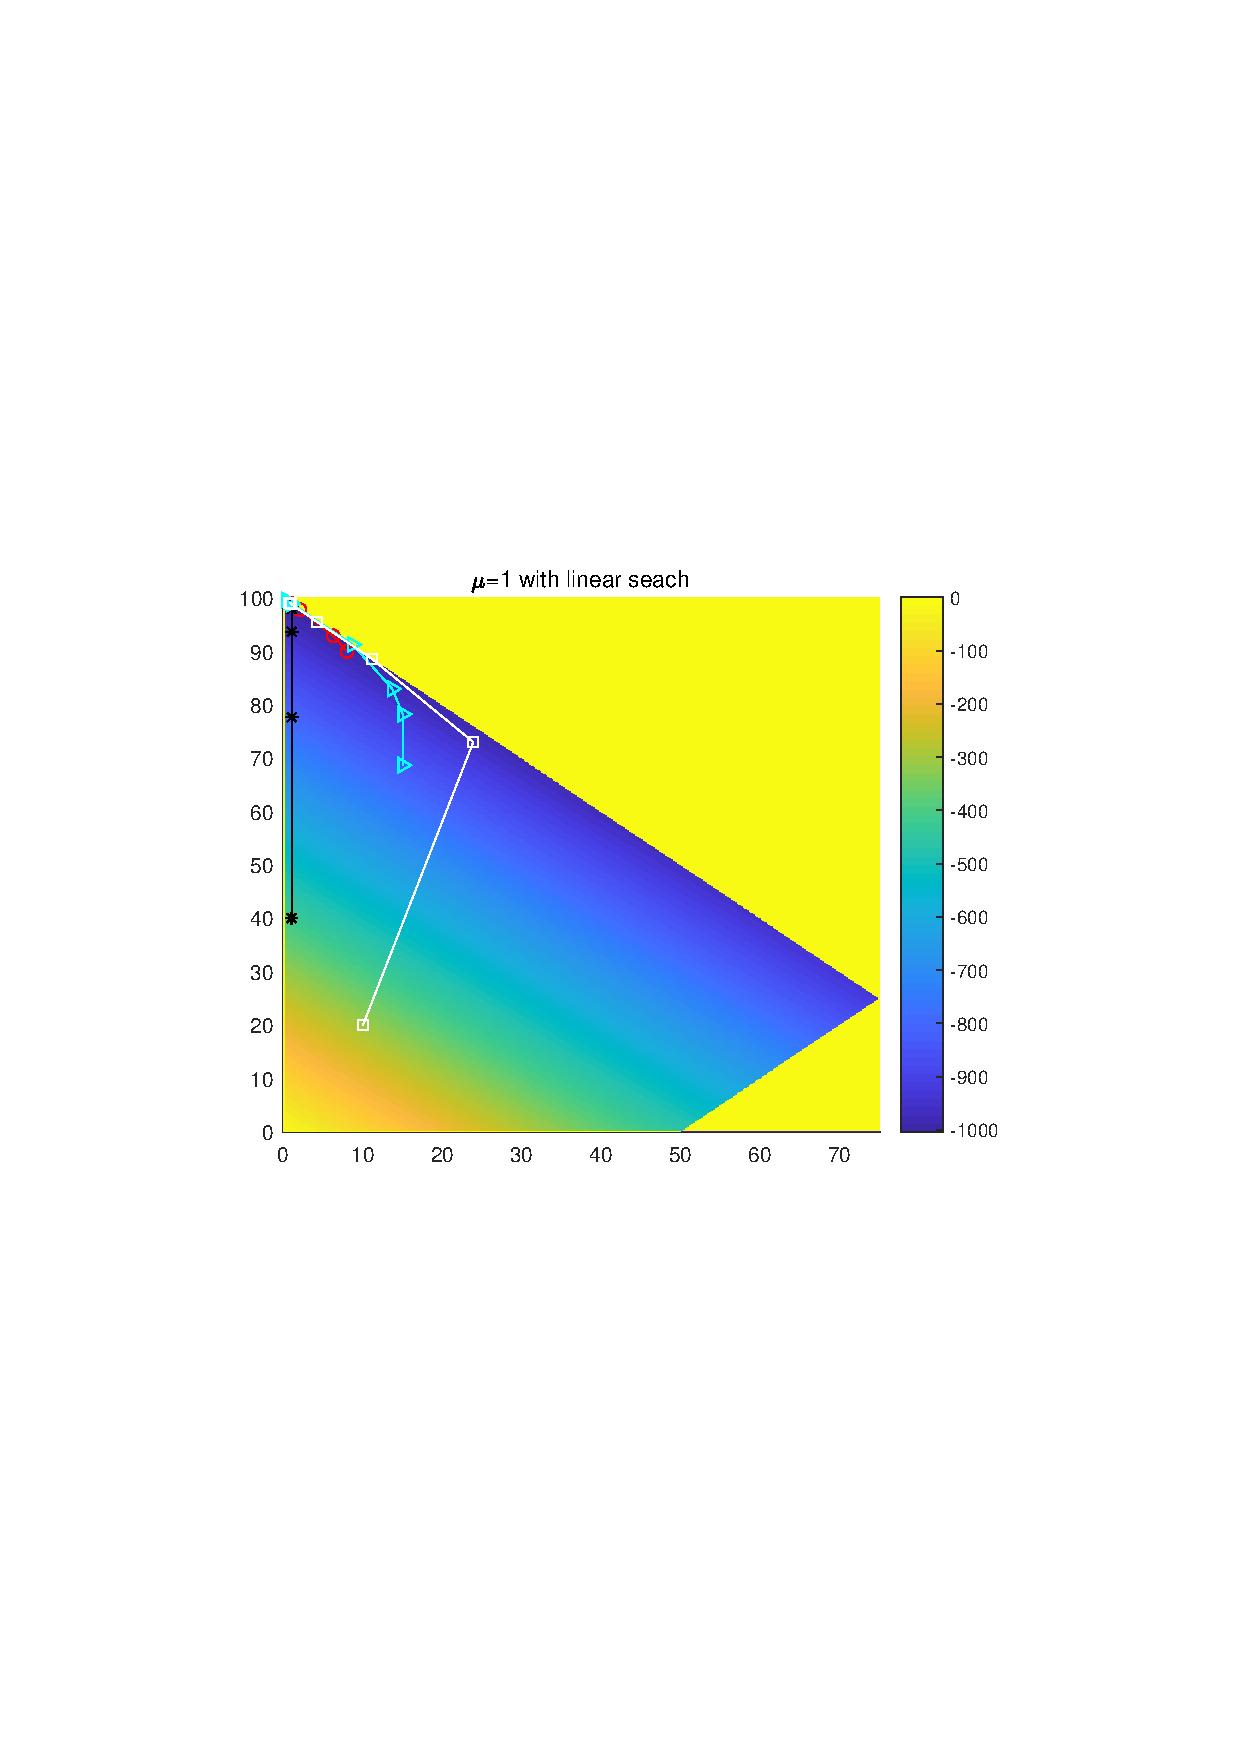
\includegraphics[width=11cm]{fig/3_1.pdf}
\end{figure}

\begin{figure}[H]
\centering
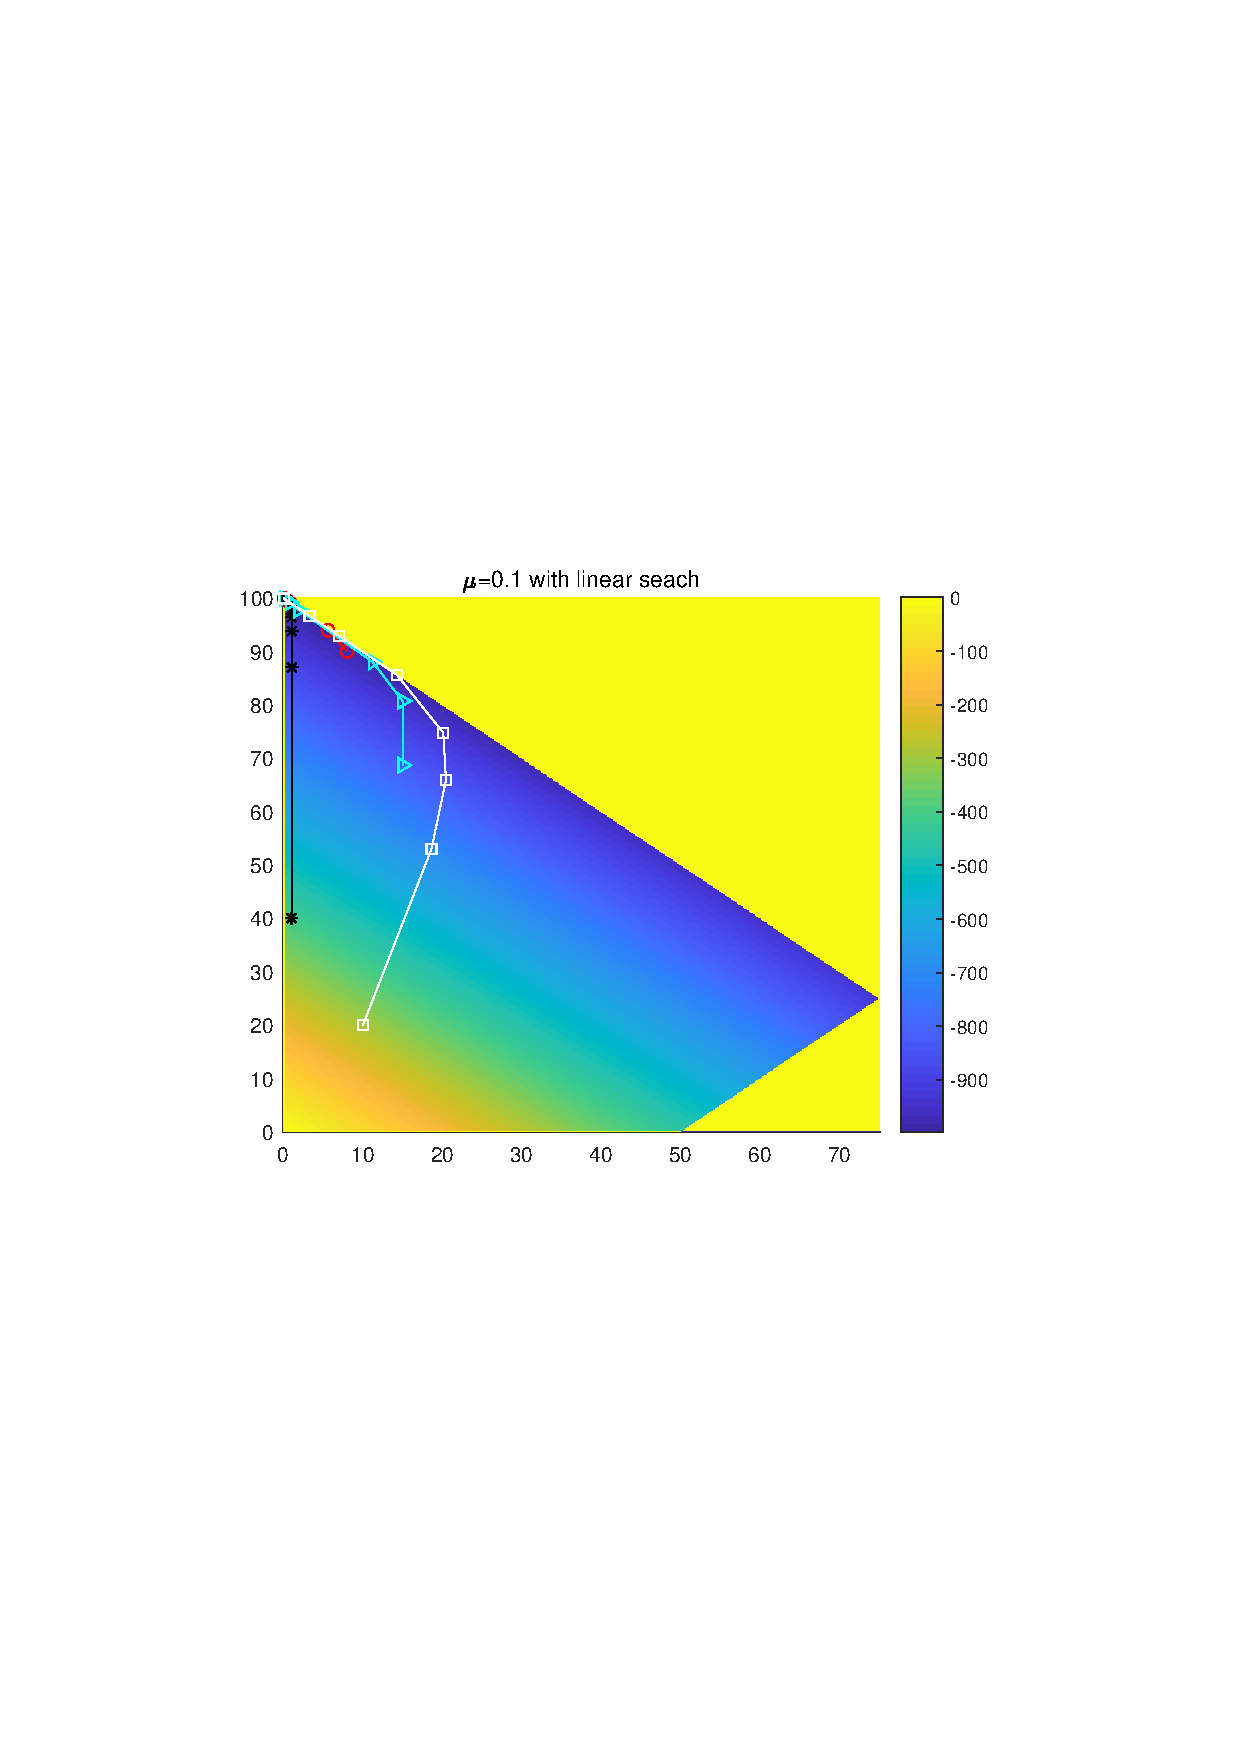
\includegraphics[width=11cm]{fig/3_2.pdf}
\end{figure}

\subsection{总结分析}
本题中Armijo线搜索的参数为$\gamma=0.5,\rho=0.01$

没加线搜索和越界判定之前,牛顿法总是一两次就冲到了定义域外,然后无法收敛。

然后我加了个越界判定:若下一步的迭代点不在定义域内,则将步长$\alpha$缩小一半,牛顿法很好地收敛到了全局最优点。

\begin{lstlisting}
%Check函数检查是否越界,以缩短步长ak
while(Check(x+ak*double(p')))
	ak=0.5*ak;
	xk=x+ak*double(p');
end
\end{lstlisting}

而后在越界判定的基础上加了个线搜索:

\begin{lstlisting}
%采用Armijo法则计算近似步长ak
while(F(xk(1),xk(2)) > (F(x(1),x(2))+0.01*double(p'*g)*ak)
||Check(x+ak*double(p')))%Check函数检查是否越界
	ak=0.5*ak;
	xk=x+ak*double(p');
end
\end{lstlisting}

然而得到的结果与加上线搜索之前一样,可见在迭代的前期,越界判定起到了一定类似于线搜索缩短步长的效果,而到了迭代的后期,牛顿法的基本步长已经满足Armijo法则,还原成了基本牛顿法。

\newpage
\section{Problem5.9}
\subsection{Rosenbrock函数图像}
首先画出Rosenbrock函数的图像及等值线如下\footnote{由于Rosenbrock函数过于陡峭,因此对原函数进行了取对数处理,以便于观察其特点。}:


\begin{figure}[H]
\centering
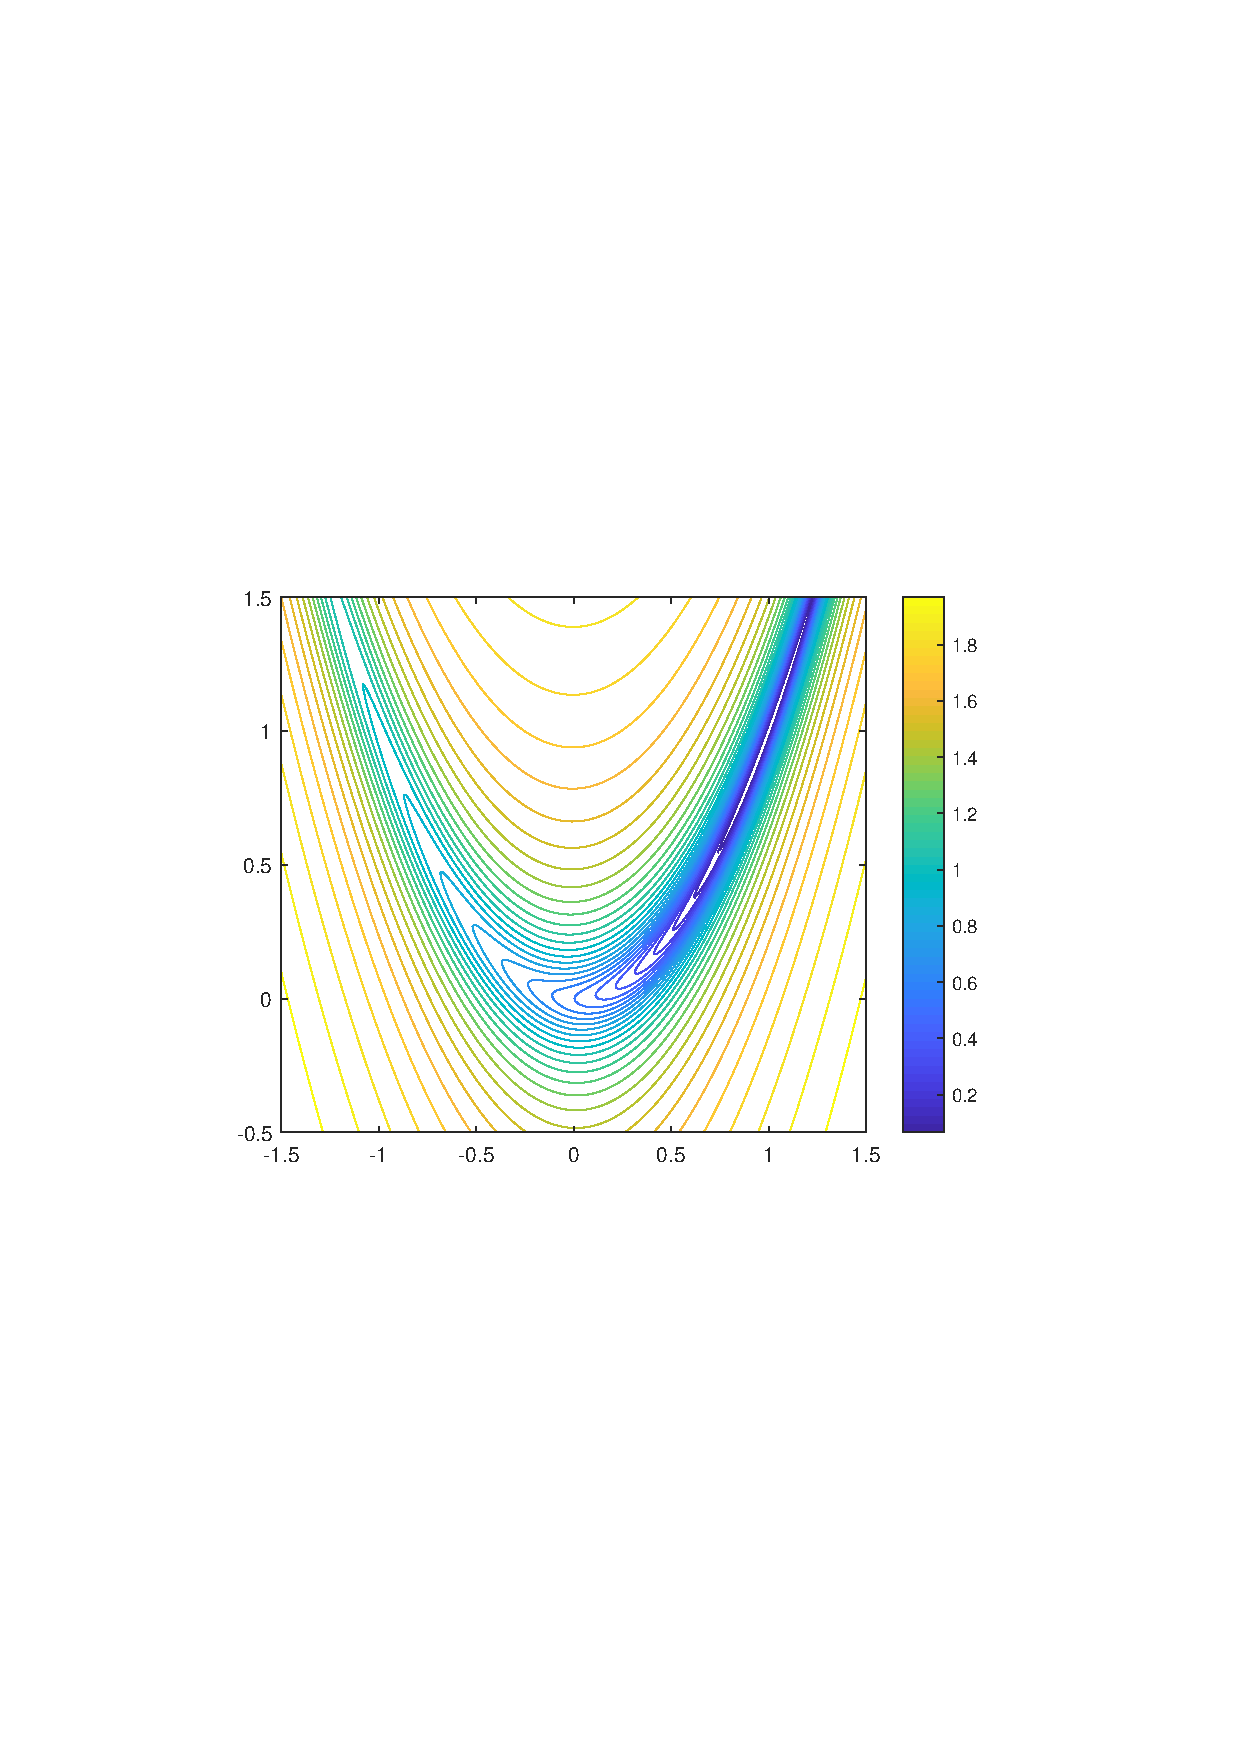
\includegraphics[width=11cm]{fig/4_01.pdf}
\end{figure}


\begin{figure}[H]
\centering
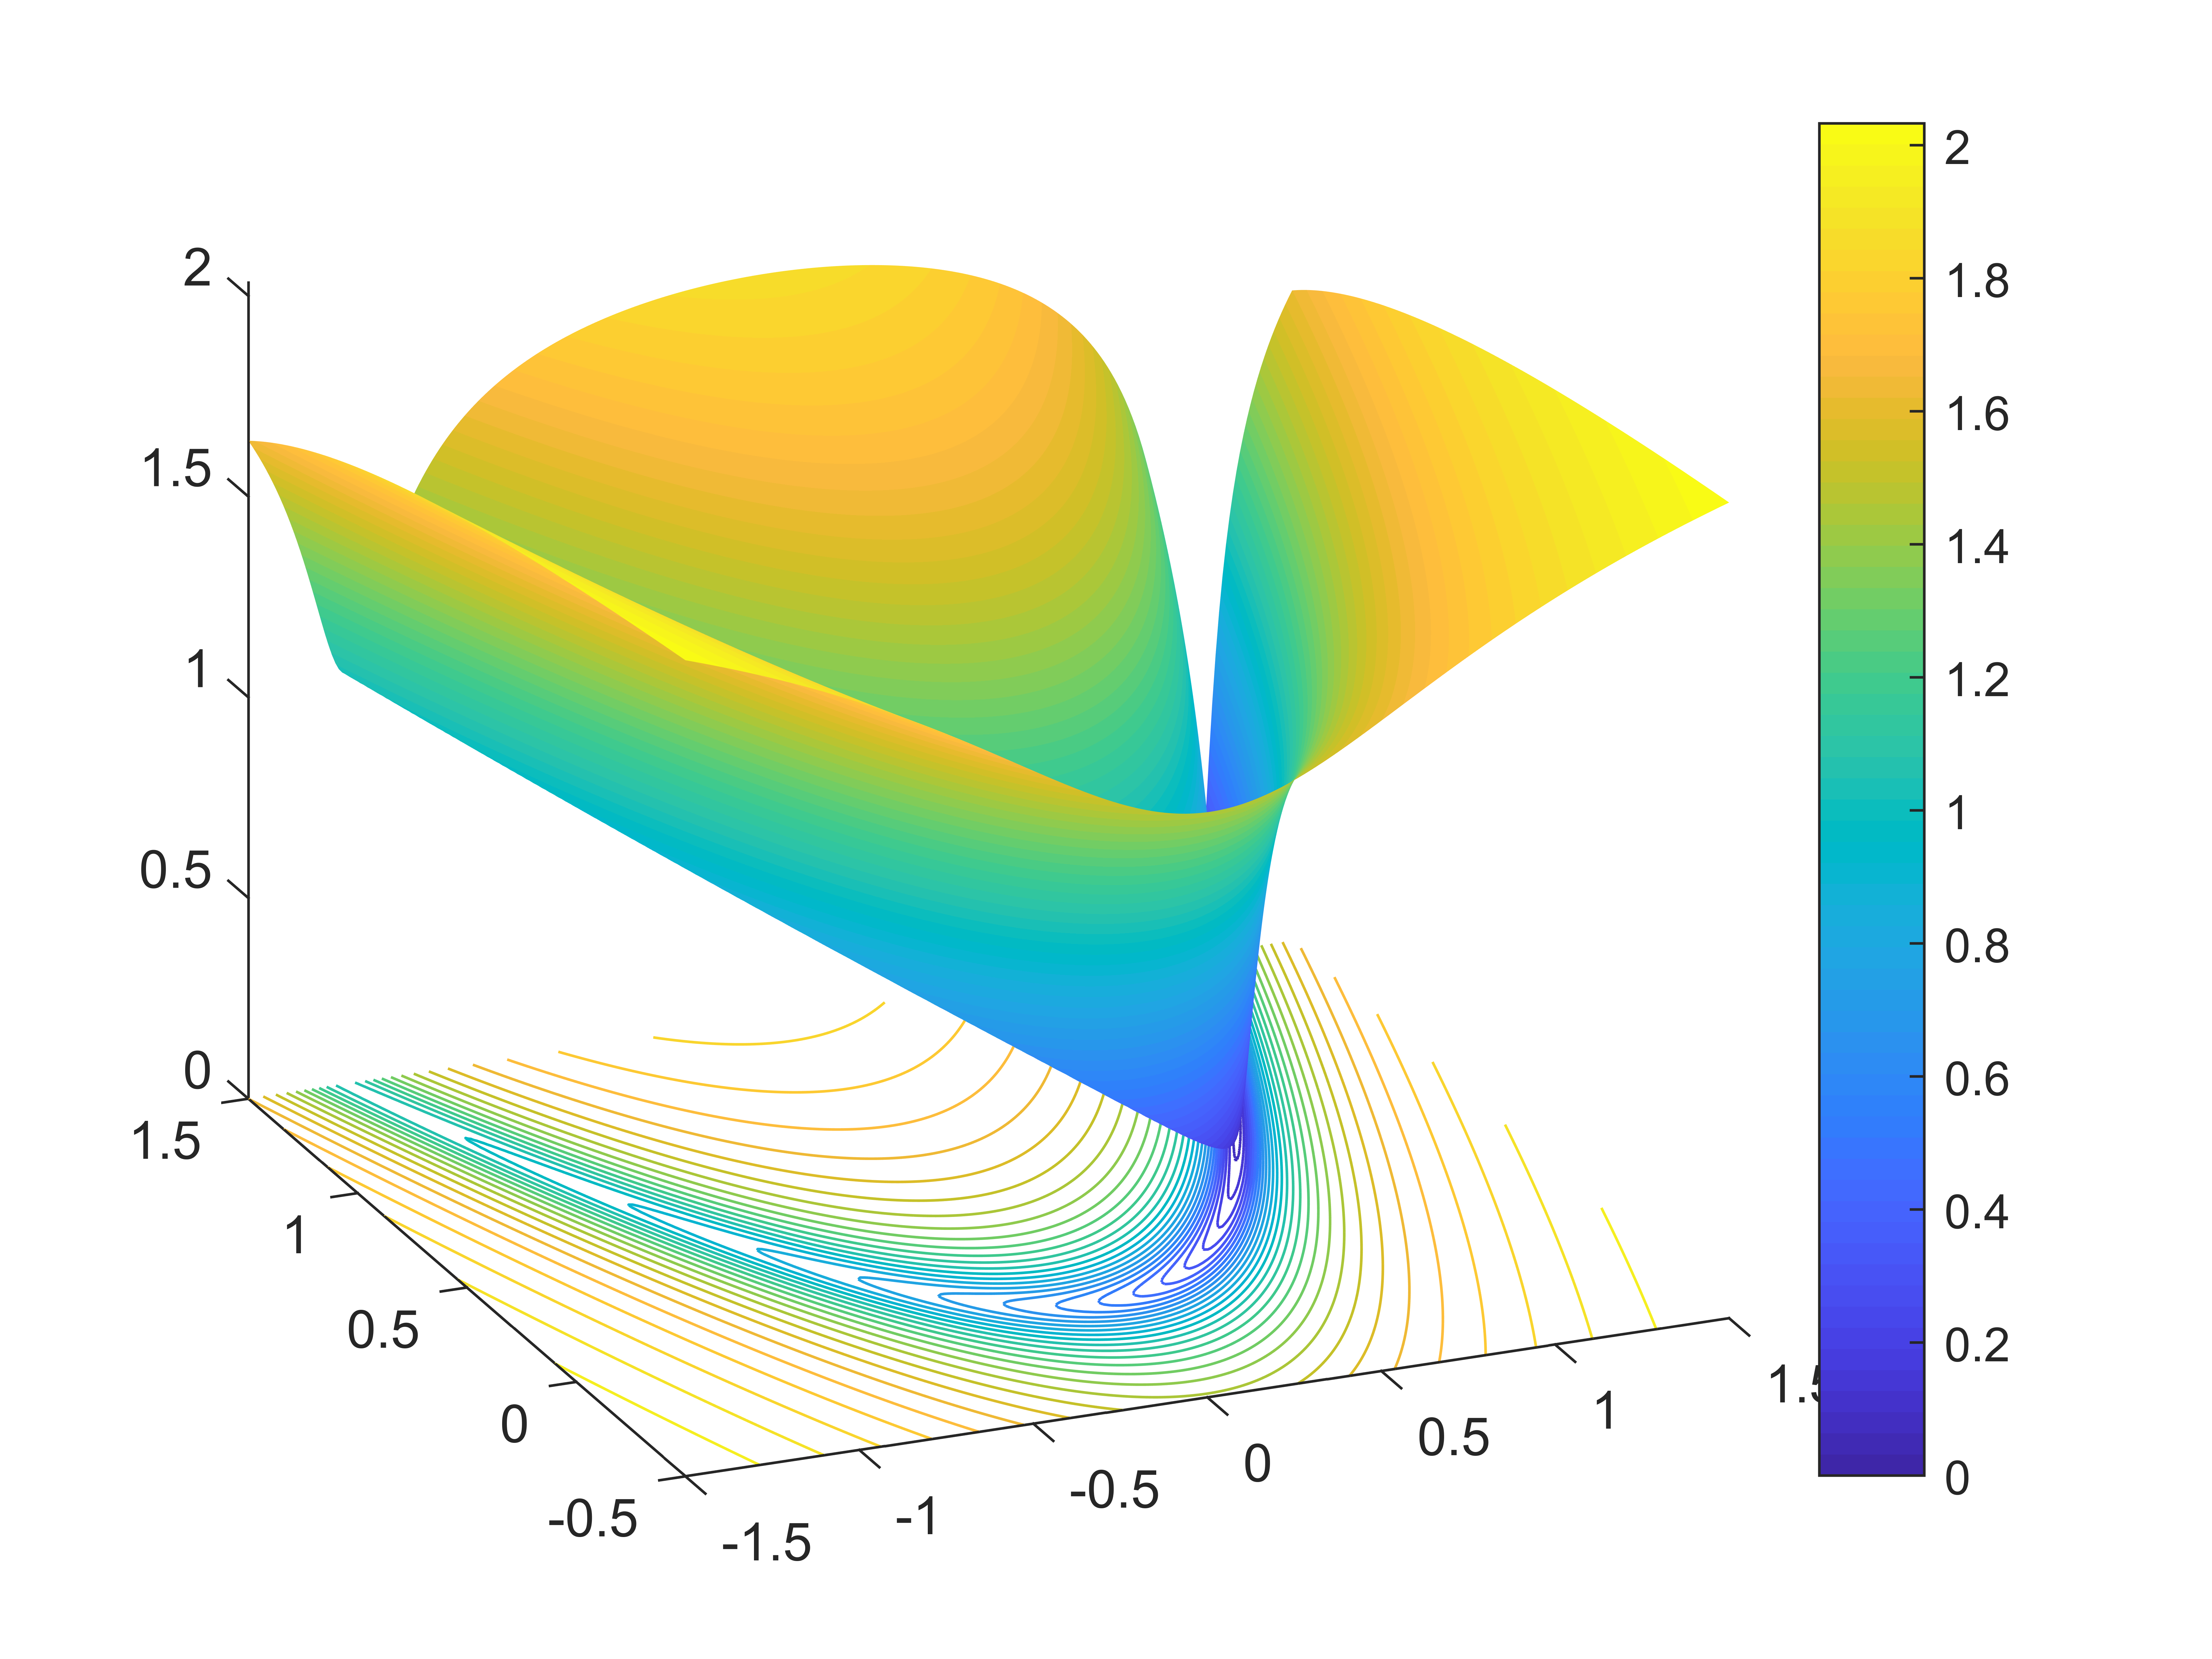
\includegraphics[width=11cm]{fig/4_02.png}
\end{figure}

\subsection{算法伪代码}
Armijo线搜索法参看上节的(\textbf{Algorithm} \ref{Amj})

带线搜索的Newton法算法参看上节的(\textbf{Algorithm} \ref{NewtonAmj})

\begin{algorithm}[h]  
\caption{Steepest-denscent-Armijo method for problem(5.9)}  
\begin{algorithmic}[1]  
\STATE Given $\bm{x}^{(0)}$ and $G$
\STATE Set $\bm{p}^{(0)}=-\bm{g}^{(0)},k=0$
\WHILE {$\|\bm{g}^{(k)}\|>\epsilon$}
\STATE Compute $\alpha_k$ by Line Search(\textbf{Algorithm} \ref{Amj})
\STATE Set $\bm{x}^{(k+1)}=\bm{x}^{(k)}+\alpha_k\bm{p}^{(k)}$
\STATE Set $\bm{g}^{(k+1)}=g(\bm{x}^{(k+1)})$
\STATE Set $\bm{p}^{(k)}=-\bm{g}^{(k)}$
\STATE Set $k=k+1$
\ENDWHILE
\end{algorithmic}  
\end{algorithm}



\subsection{计算结果展示}

本题中Armijo线搜索的参数为$\gamma=0.5,\rho=0.01$,并设置最大搜索步长为200.

然后分别以梯度下降法和牛顿法迭代,并画出等高线、运动轨迹、迭代值如下:

\begin{figure}[H]
\centering
\subfigure{
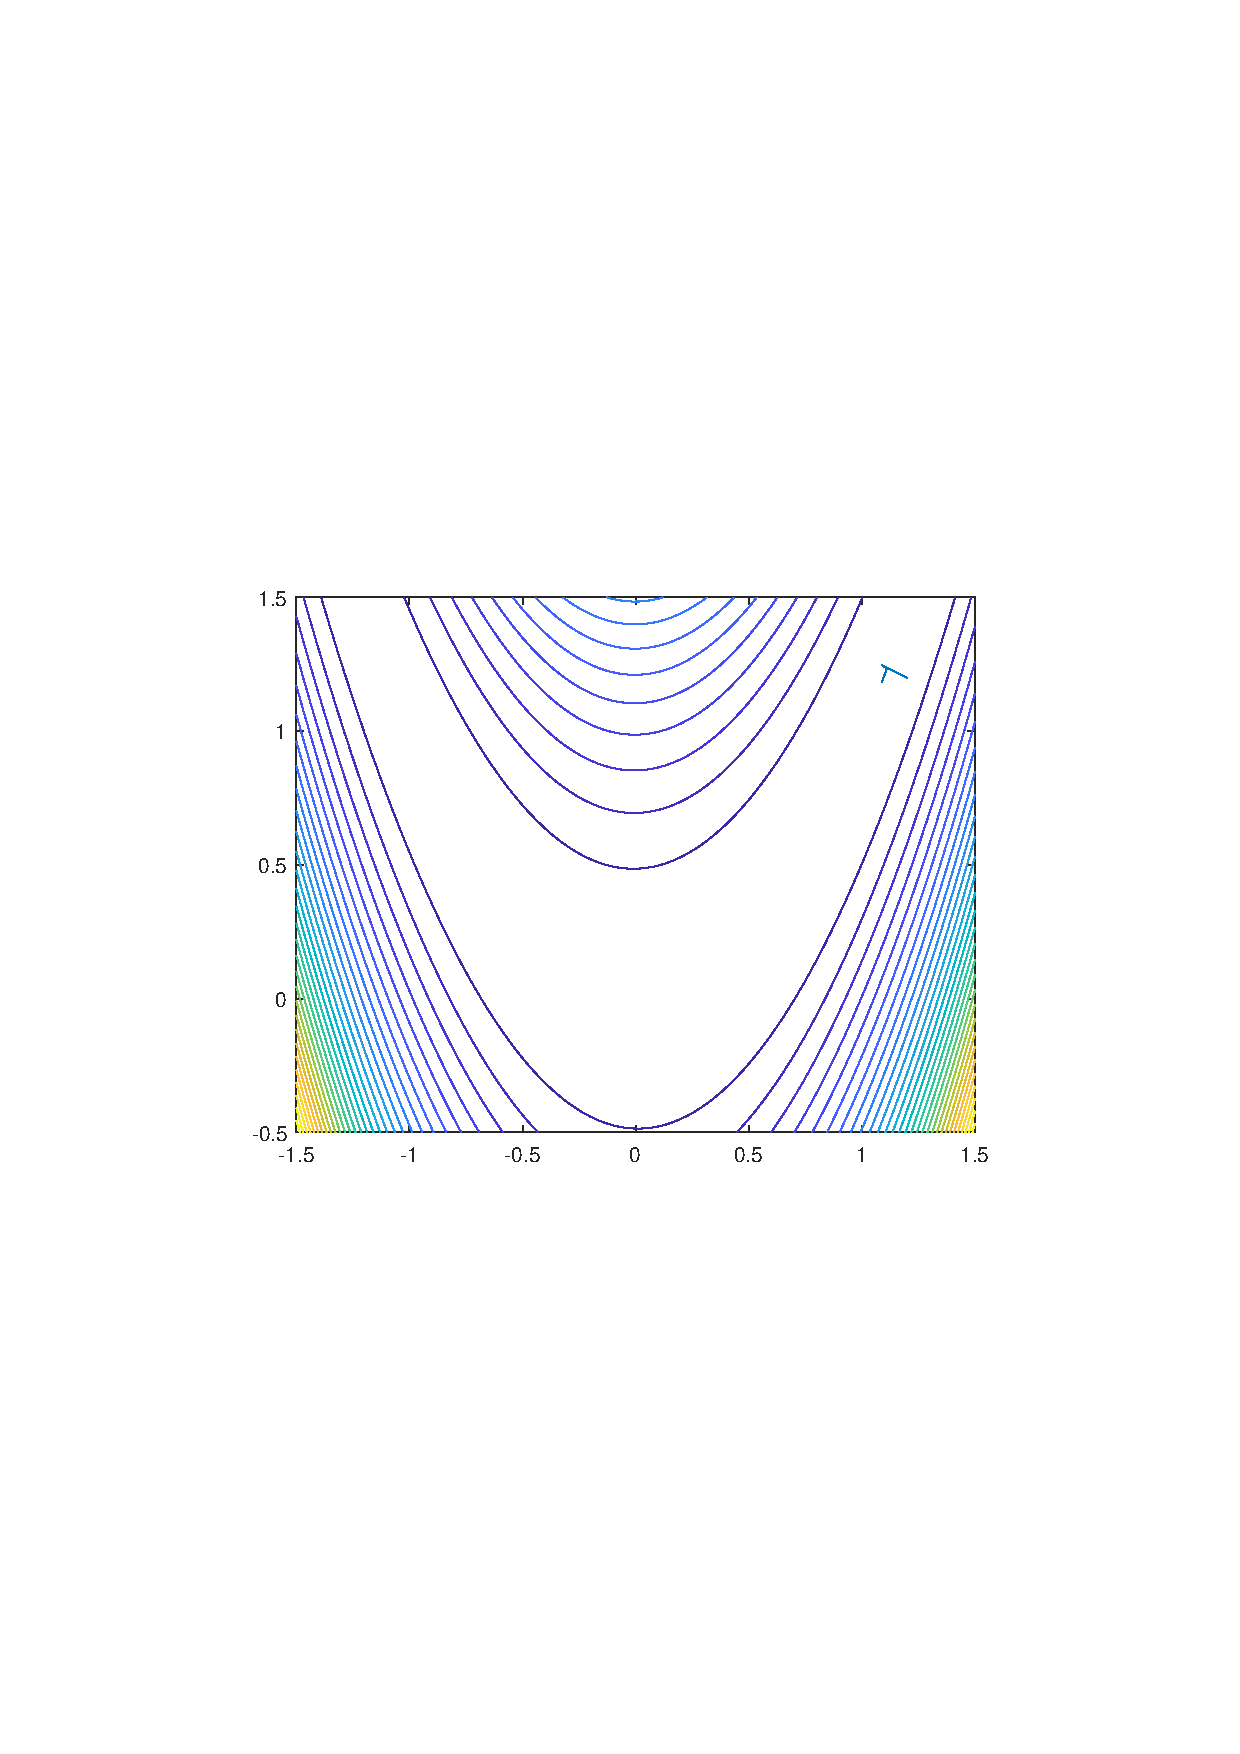
\includegraphics[width=5cm]{fig/4_11.pdf}}
\subfigure{
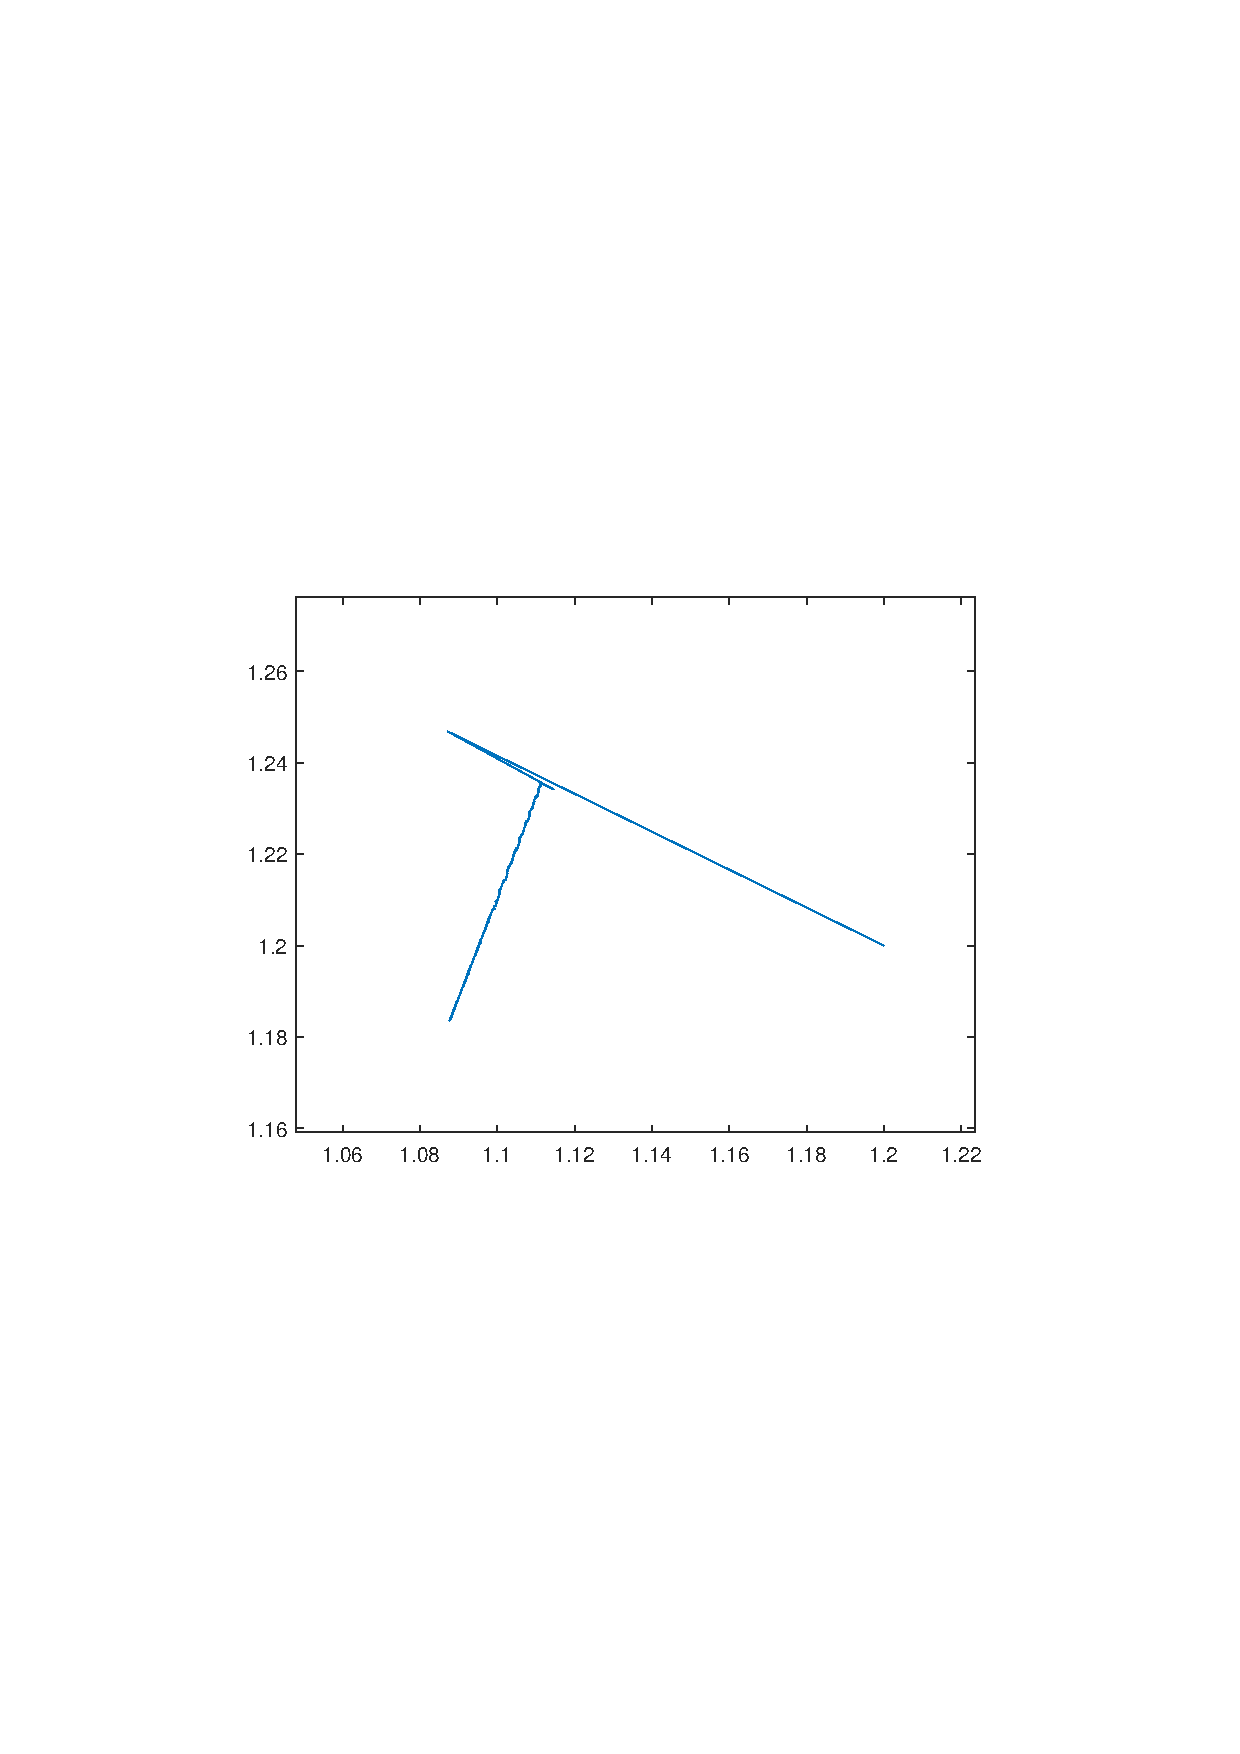
\includegraphics[width=5cm]{fig/4_12.pdf}}
\subfigure{
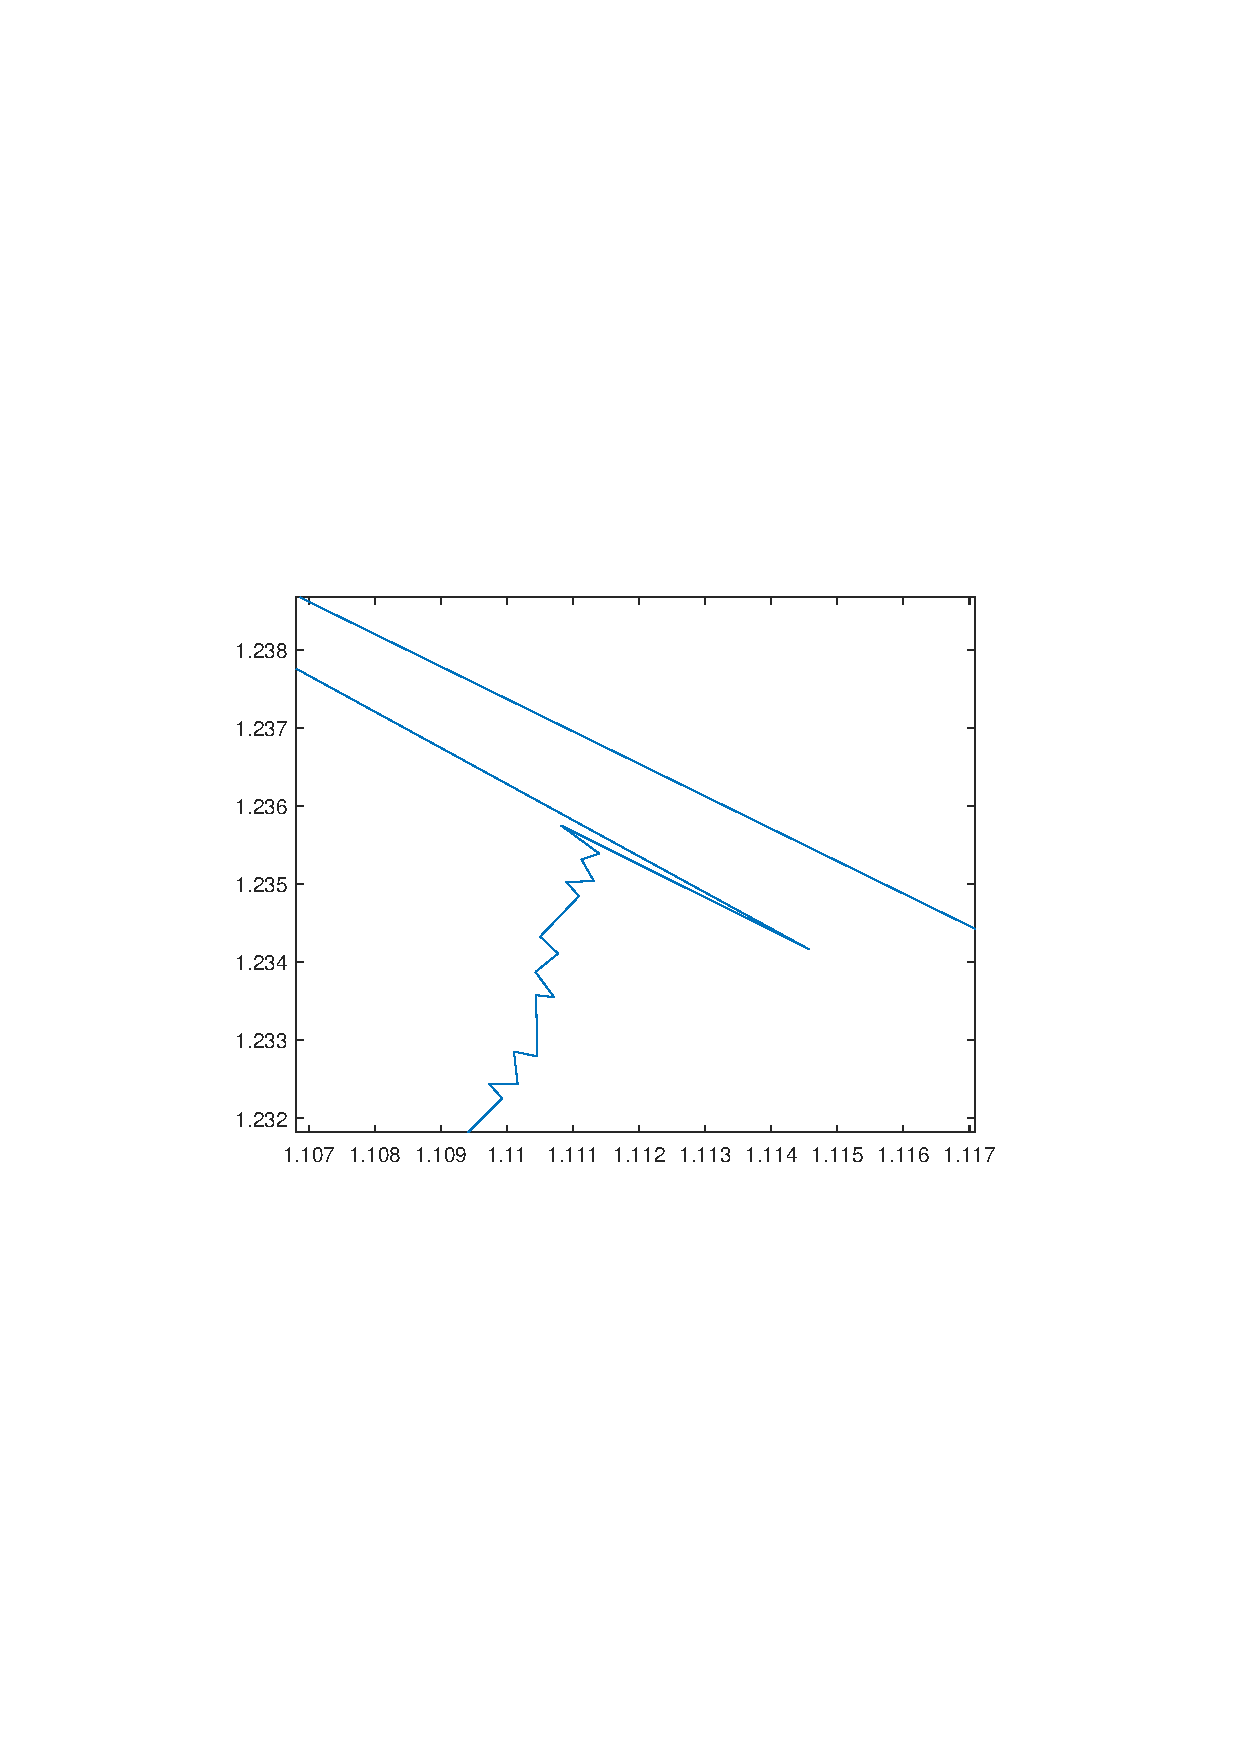
\includegraphics[width=5cm]{fig/4_13.pdf}}
\subfigure{
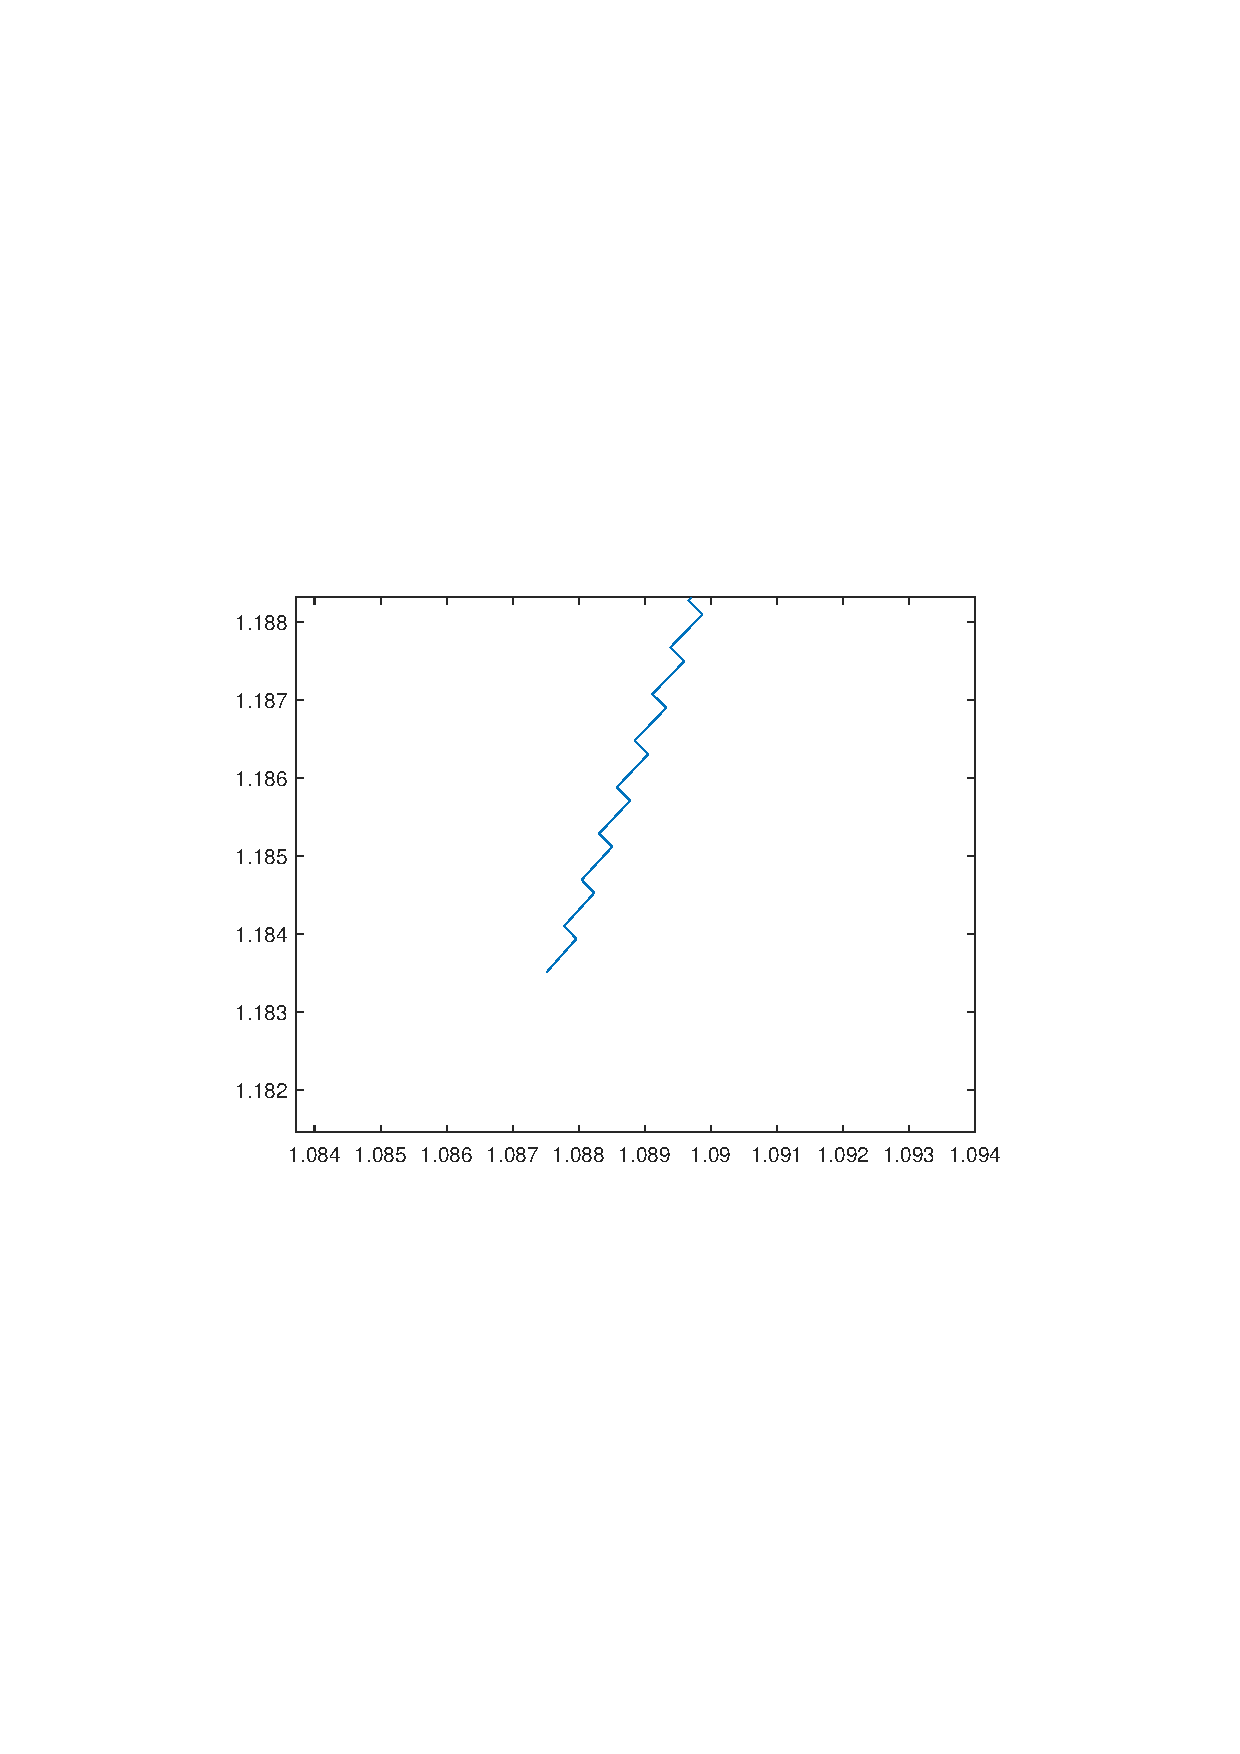
\includegraphics[width=5cm]{fig/4_14.pdf}}
\caption{Steepest-denscent in (1.2,1.2)}
\label{Fig.lable}
\end{figure}
\begin{lstlisting}
%Result for Steepest-denscent in (1.2,1.2)
Step[1]:  x=[ 1.200000 1.200000 ] optim_fx=5.800000
Step[2]:  x=[ 1.087109 1.246875 ] optim_fx=0.430975
Step[3]:  x=[ 1.114571 1.234166 ] optim_fx=0.019689
...
...
...
Step[198]:  x=[ 1.083582 1.174725 ] optim_fx=0.007019
Step[199]:  x=[ 1.083742 1.174500 ] optim_fx=0.007013
Step[200]:  x=[ 1.083580 1.174500 ] optim_fx=0.006998
%最速下降法,共迭代 200 步
%最优解:
x=[ 1.083580e+00 1.174500e+00 ] optim_fx=0.006998
\end{lstlisting}

\begin{figure}[H]
\centering
\subfigure{
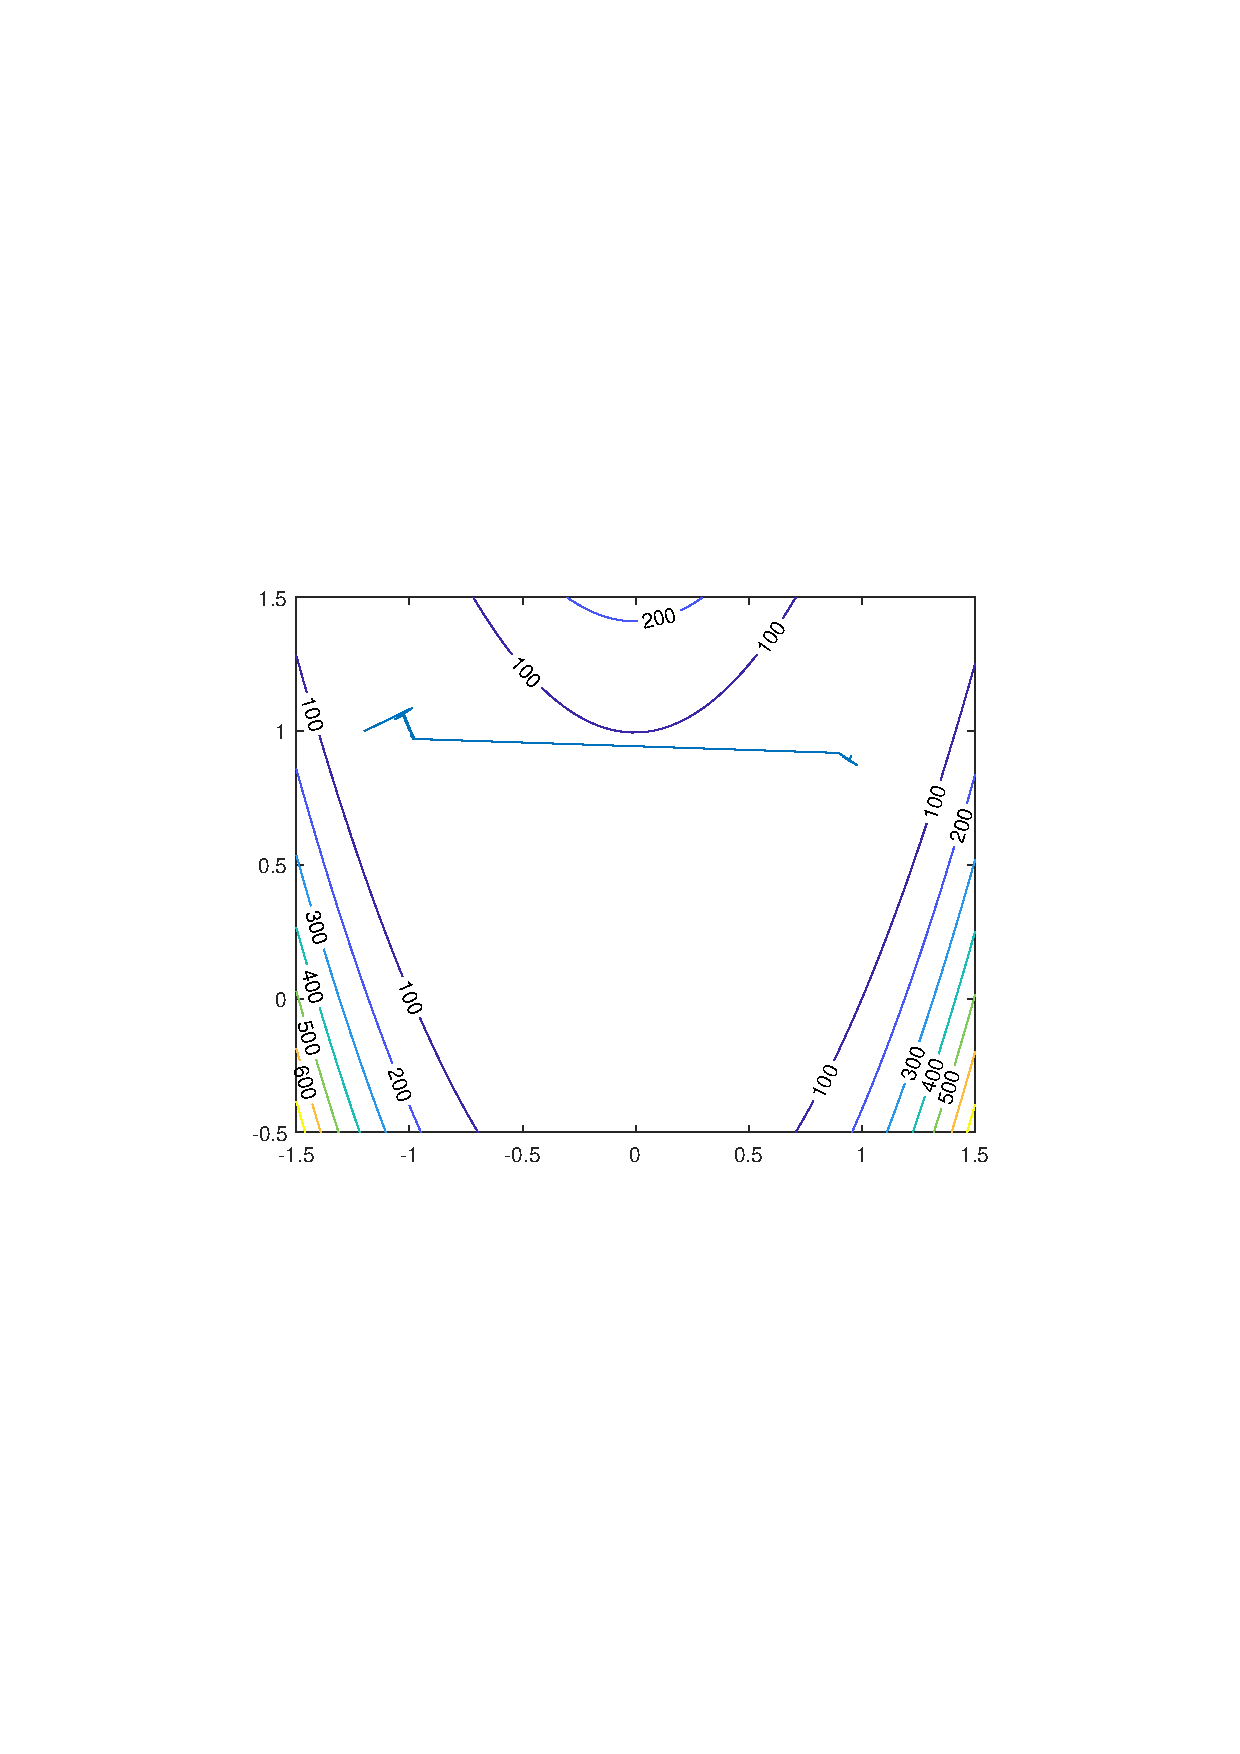
\includegraphics[width=5cm]{fig/4_21.pdf}}
\subfigure{
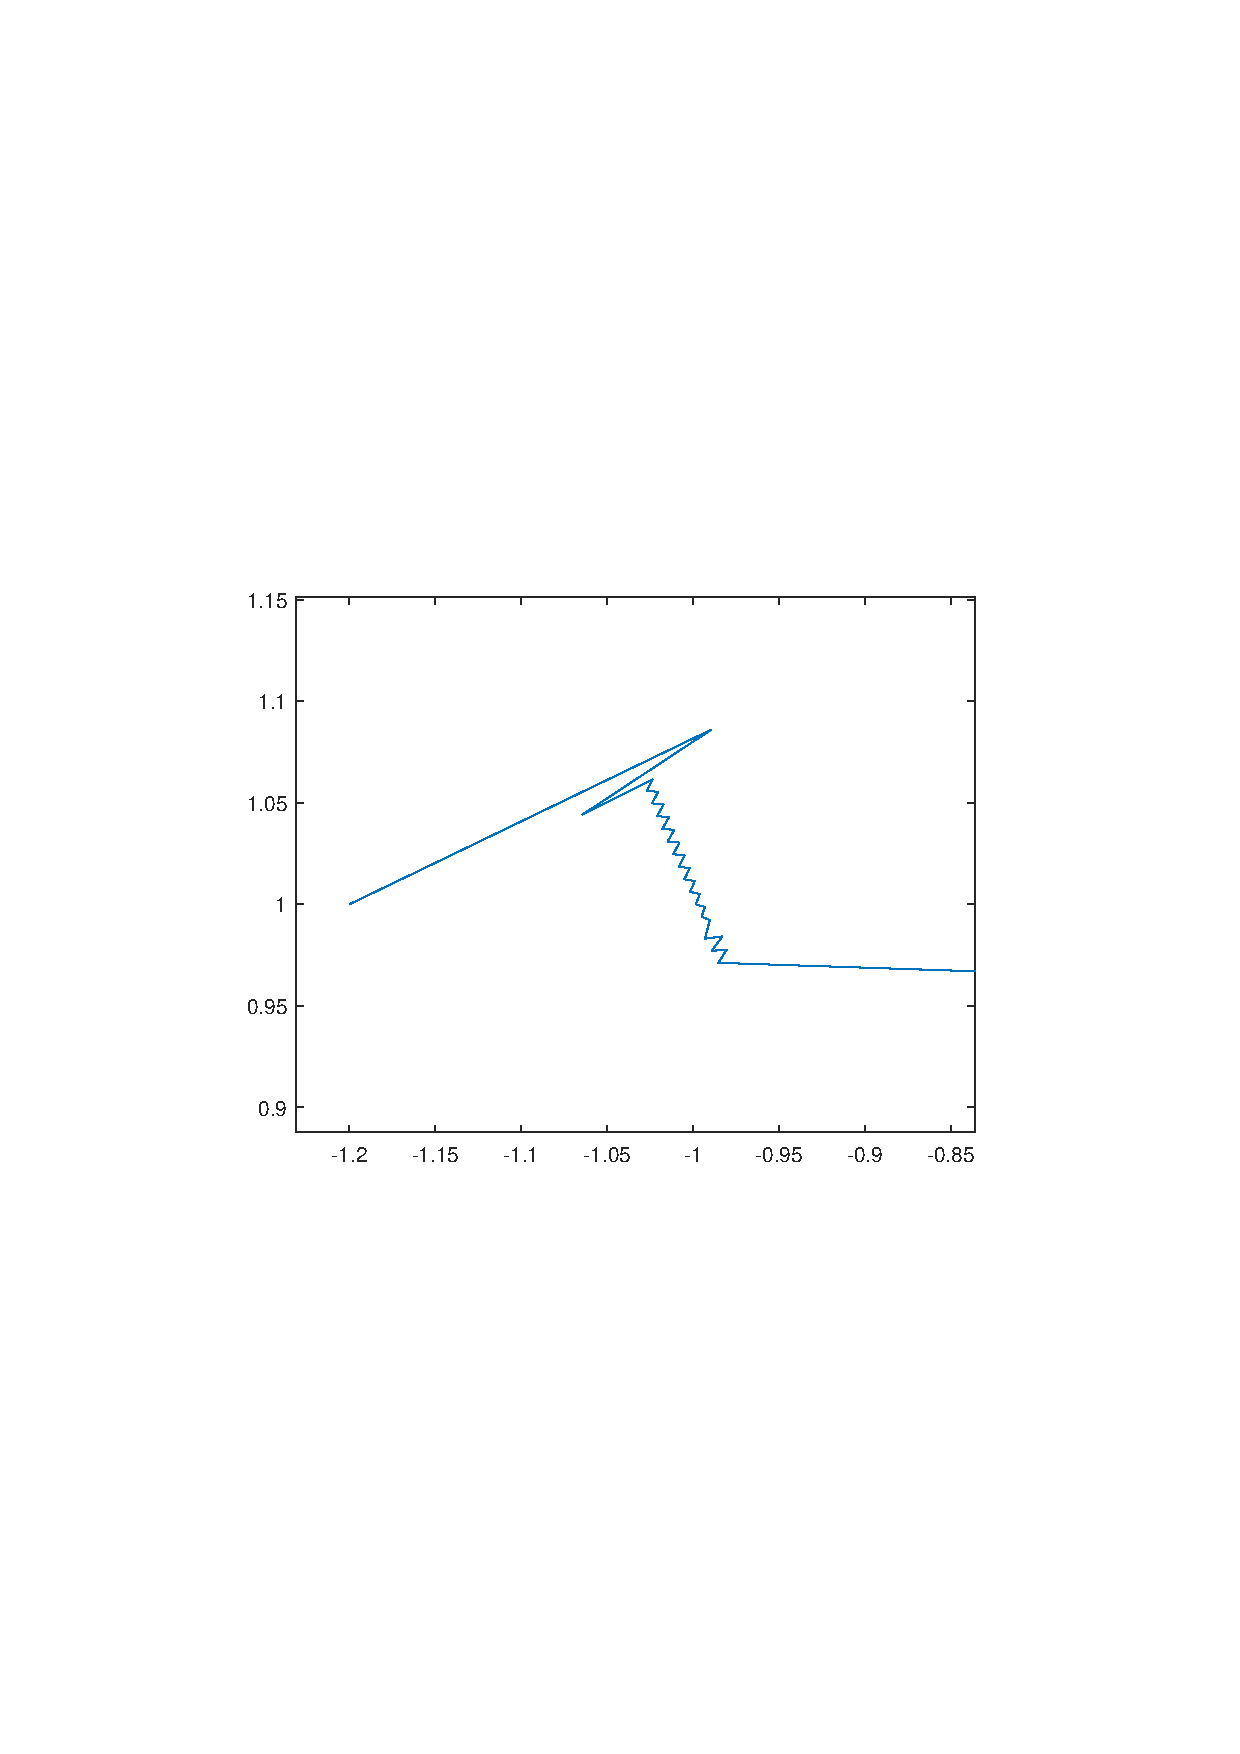
\includegraphics[width=5cm]{fig/4_22.pdf}}
\subfigure{
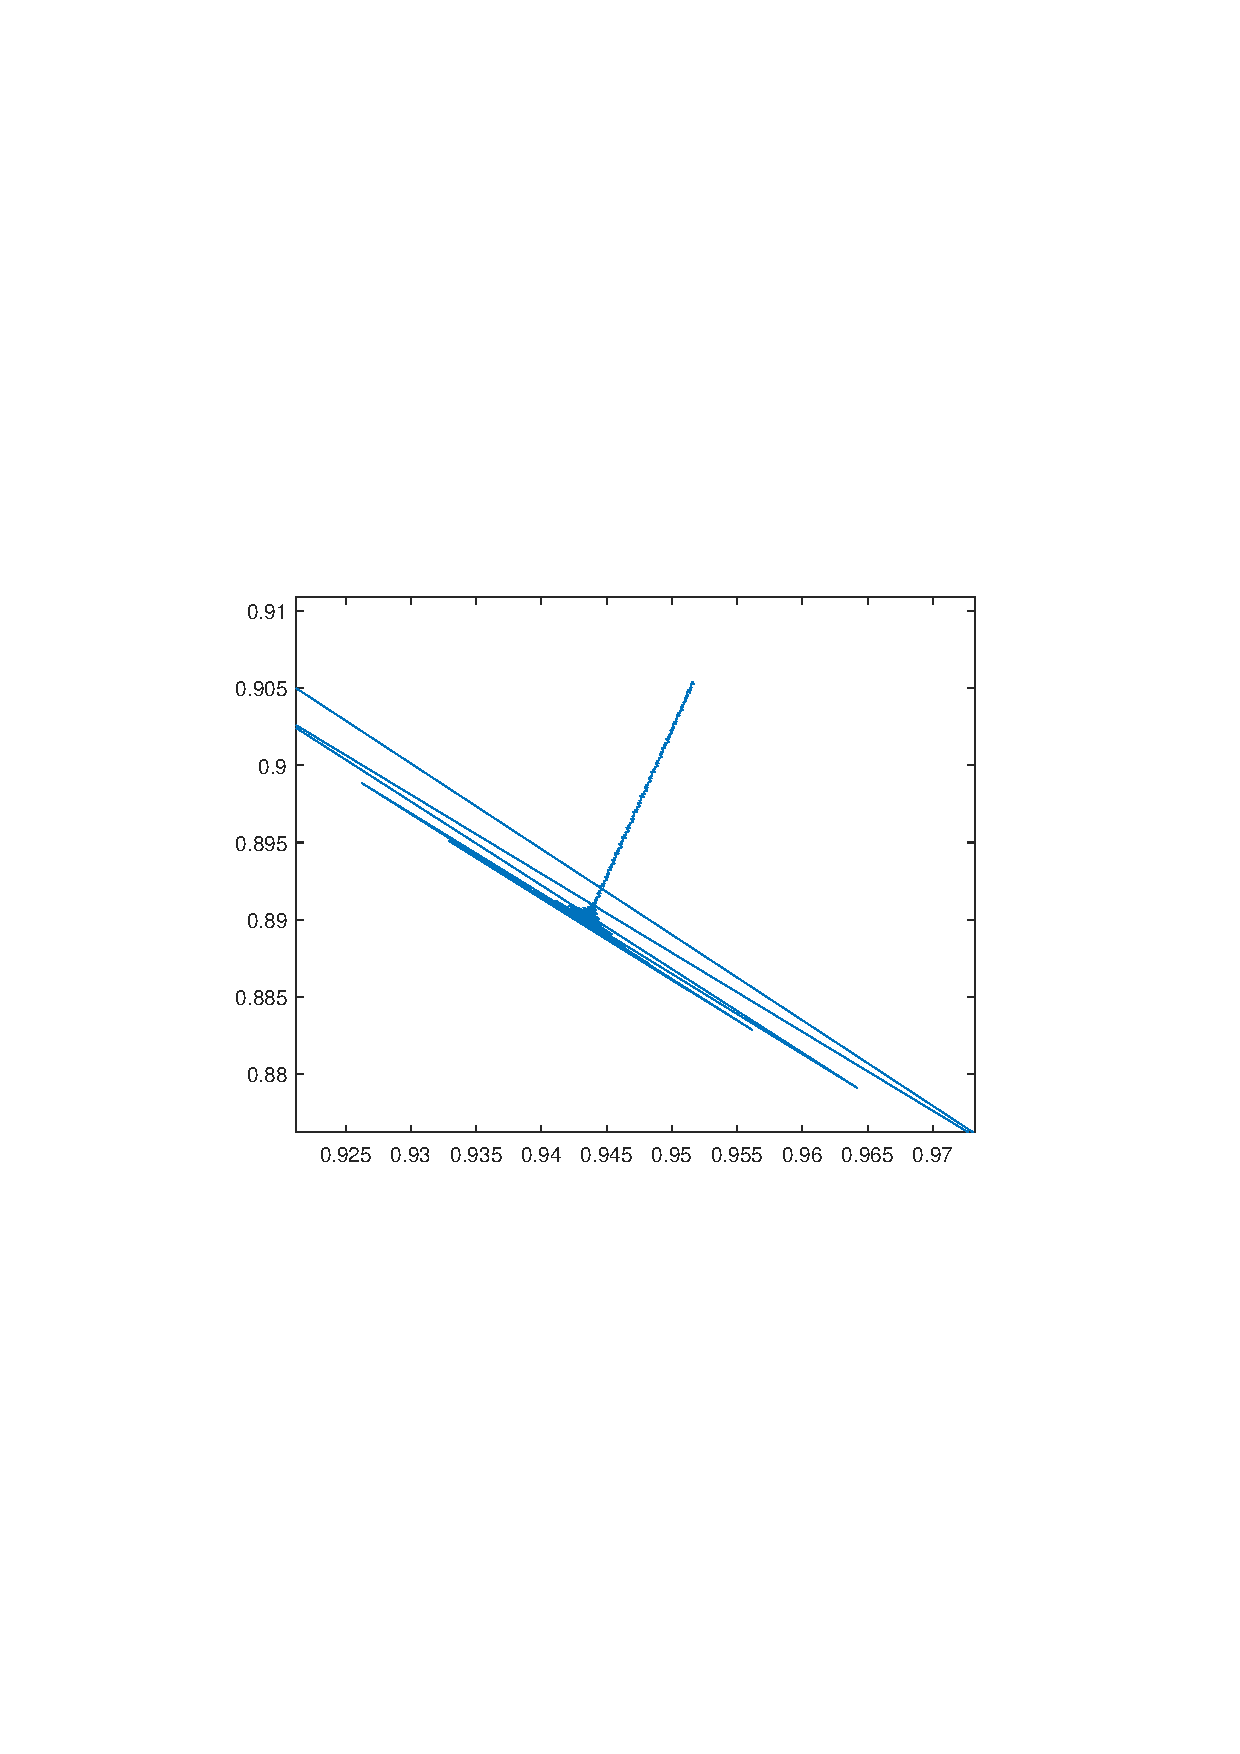
\includegraphics[width=5cm]{fig/4_23.pdf}}
\subfigure{
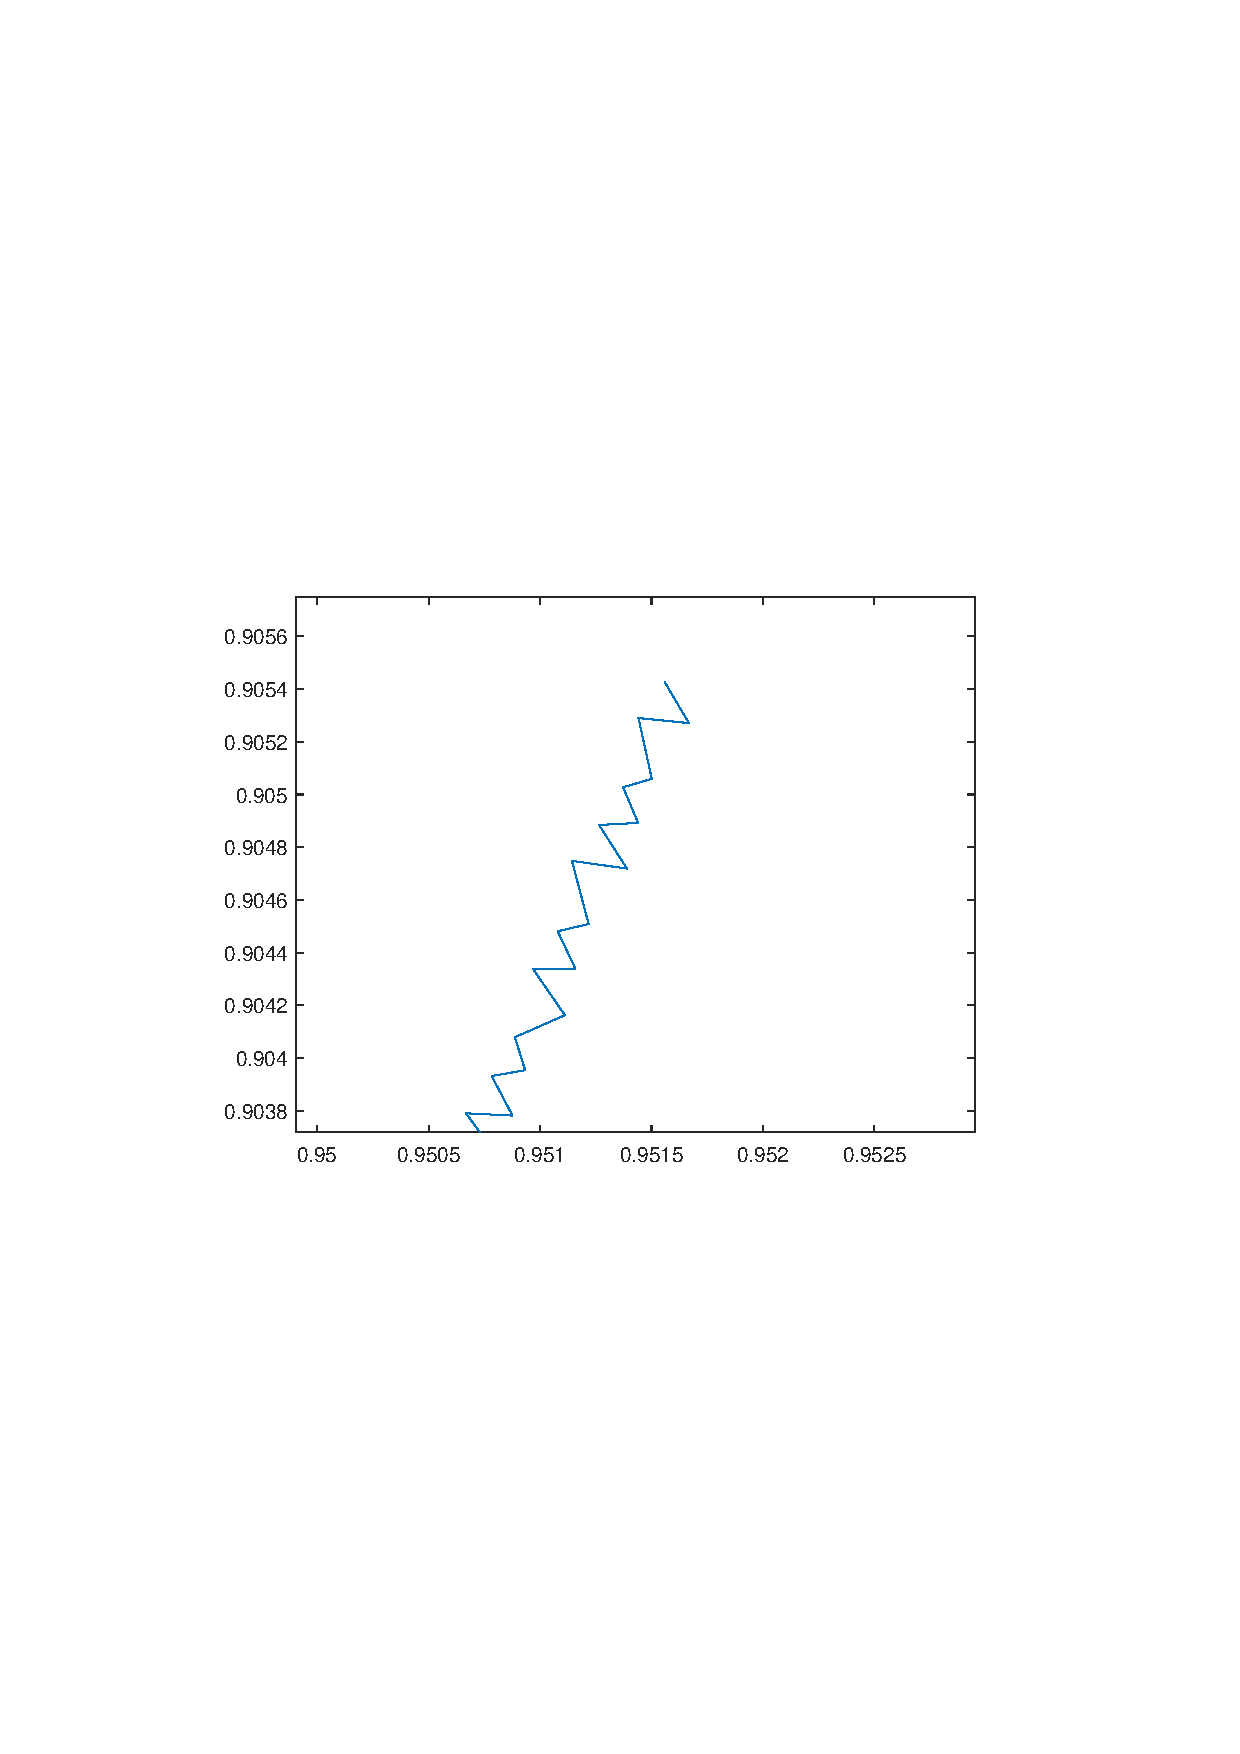
\includegraphics[width=5cm]{fig/4_24.pdf}}
\caption{Steepest-denscent in (-1.2,1)}
\label{Fig.lable}
\end{figure}

\begin{lstlisting}
%Result for Steepest-denscent in (-1.2,1)
Step[1]:  x=[ -1.200000 1.000000 ] optim_fx=24.200000
Step[2]:  x=[ -0.989453 1.085938 ] optim_fx=5.101113
Step[3]:  x=[ -1.026893 1.065055 ] optim_fx=4.119416
Step[4]:  x=[ -1.027979 1.056815 ] optim_fx=4.112700
Step[5]:  x=[ 0.984742 1.049394 ] optim_fx=0.635080
Step[6]:  x=[ 1.015421 1.033832 ] optim_fx=0.000995
...
...
...
Step[195]:  x=[ 1.005171 1.010402 ] optim_fx=0.000027
Step[196]:  x=[ 1.005177 1.010389 ] optim_fx=0.000027
Step[197]:  x=[ 1.005163 1.010386 ] optim_fx=0.000027
Step[198]:  x=[ 1.005169 1.010373 ] optim_fx=0.000027
Step[199]:  x=[ 1.005155 1.010370 ] optim_fx=0.000027
Step[200]:  x=[ 1.005161 1.010357 ] optim_fx=0.000027
%最速下降法,共迭代 200 步
%最优解:
x=[ 1.005161e+00 1.010357e+00 ] optim_fx=0.000027
\end{lstlisting}

\begin{figure}[H]
\centering
\subfigure{
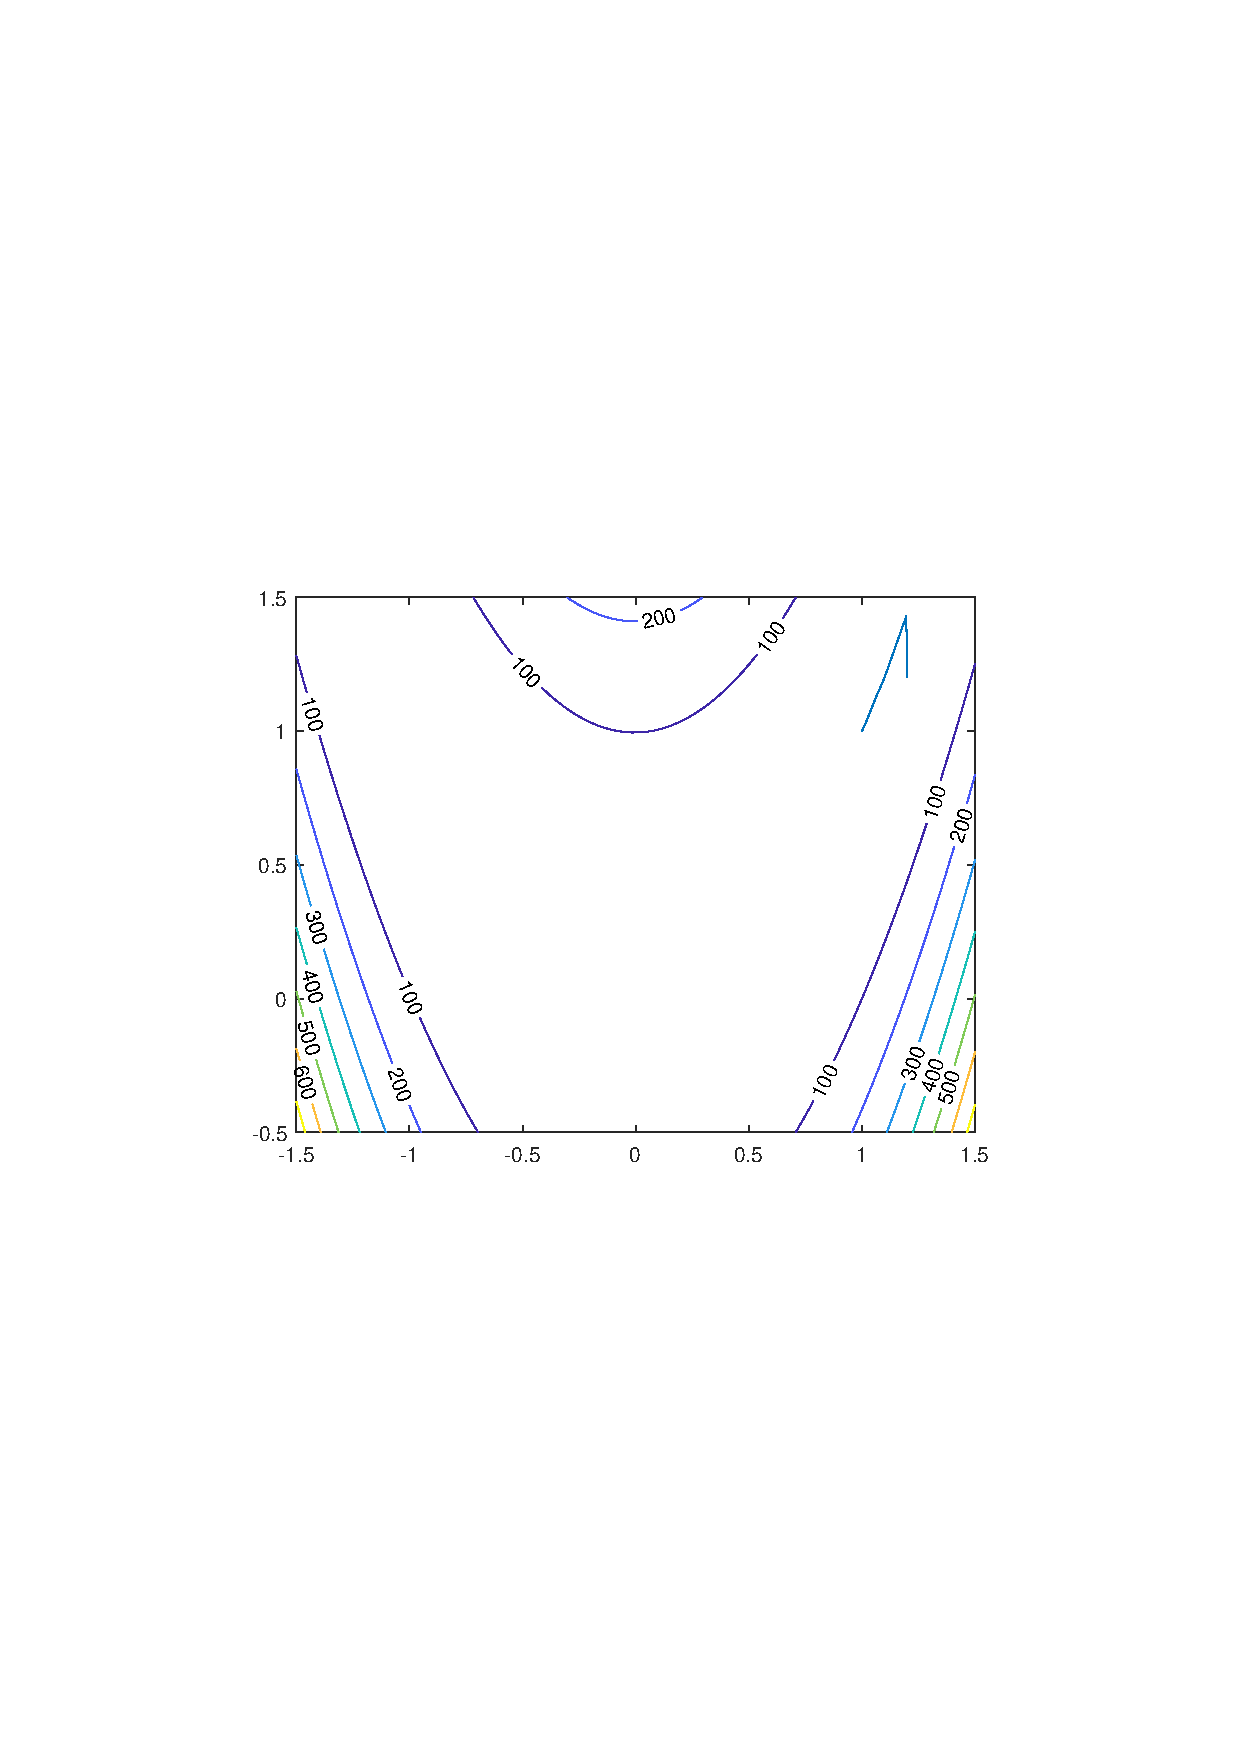
\includegraphics[width=5cm]{fig/4_31.pdf}}
\subfigure{
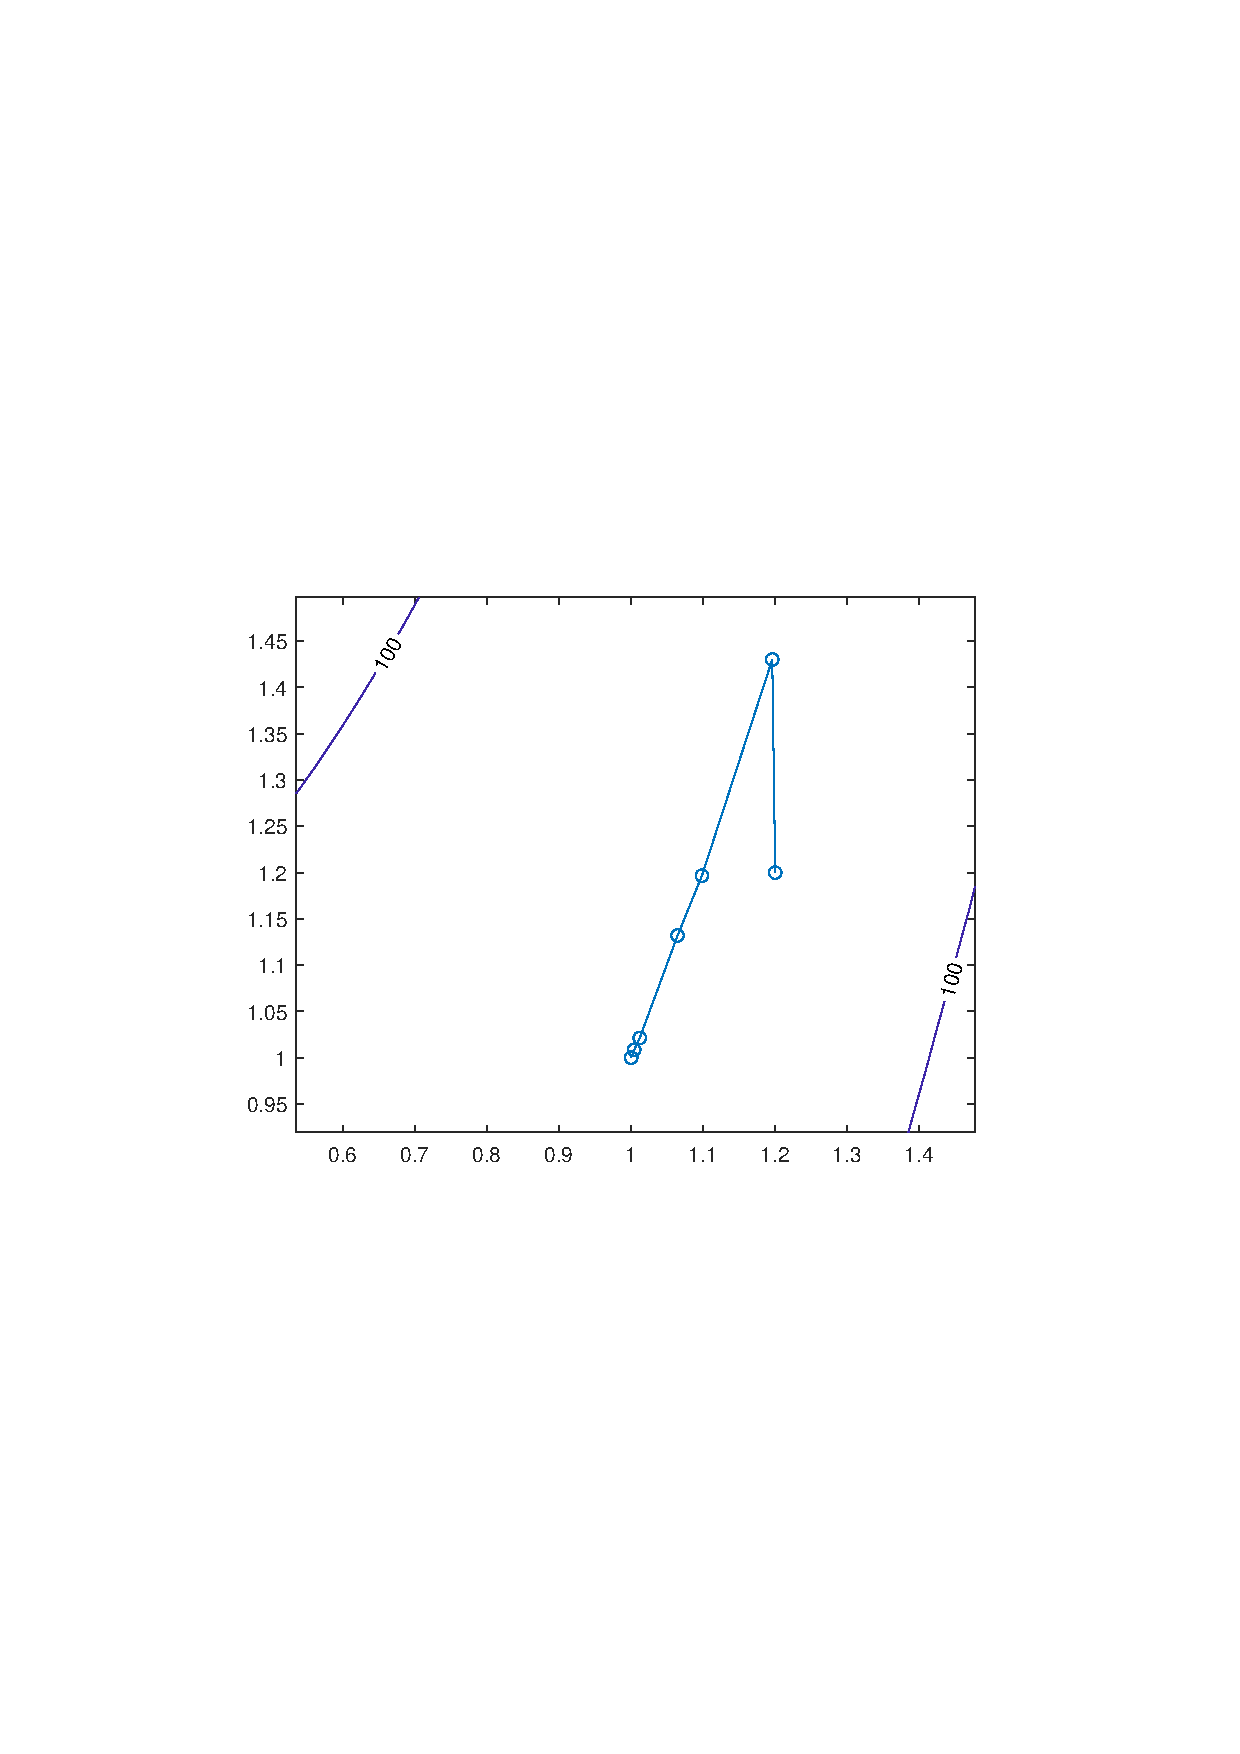
\includegraphics[width=5cm]{fig/4_32.pdf}}
\subfigure{
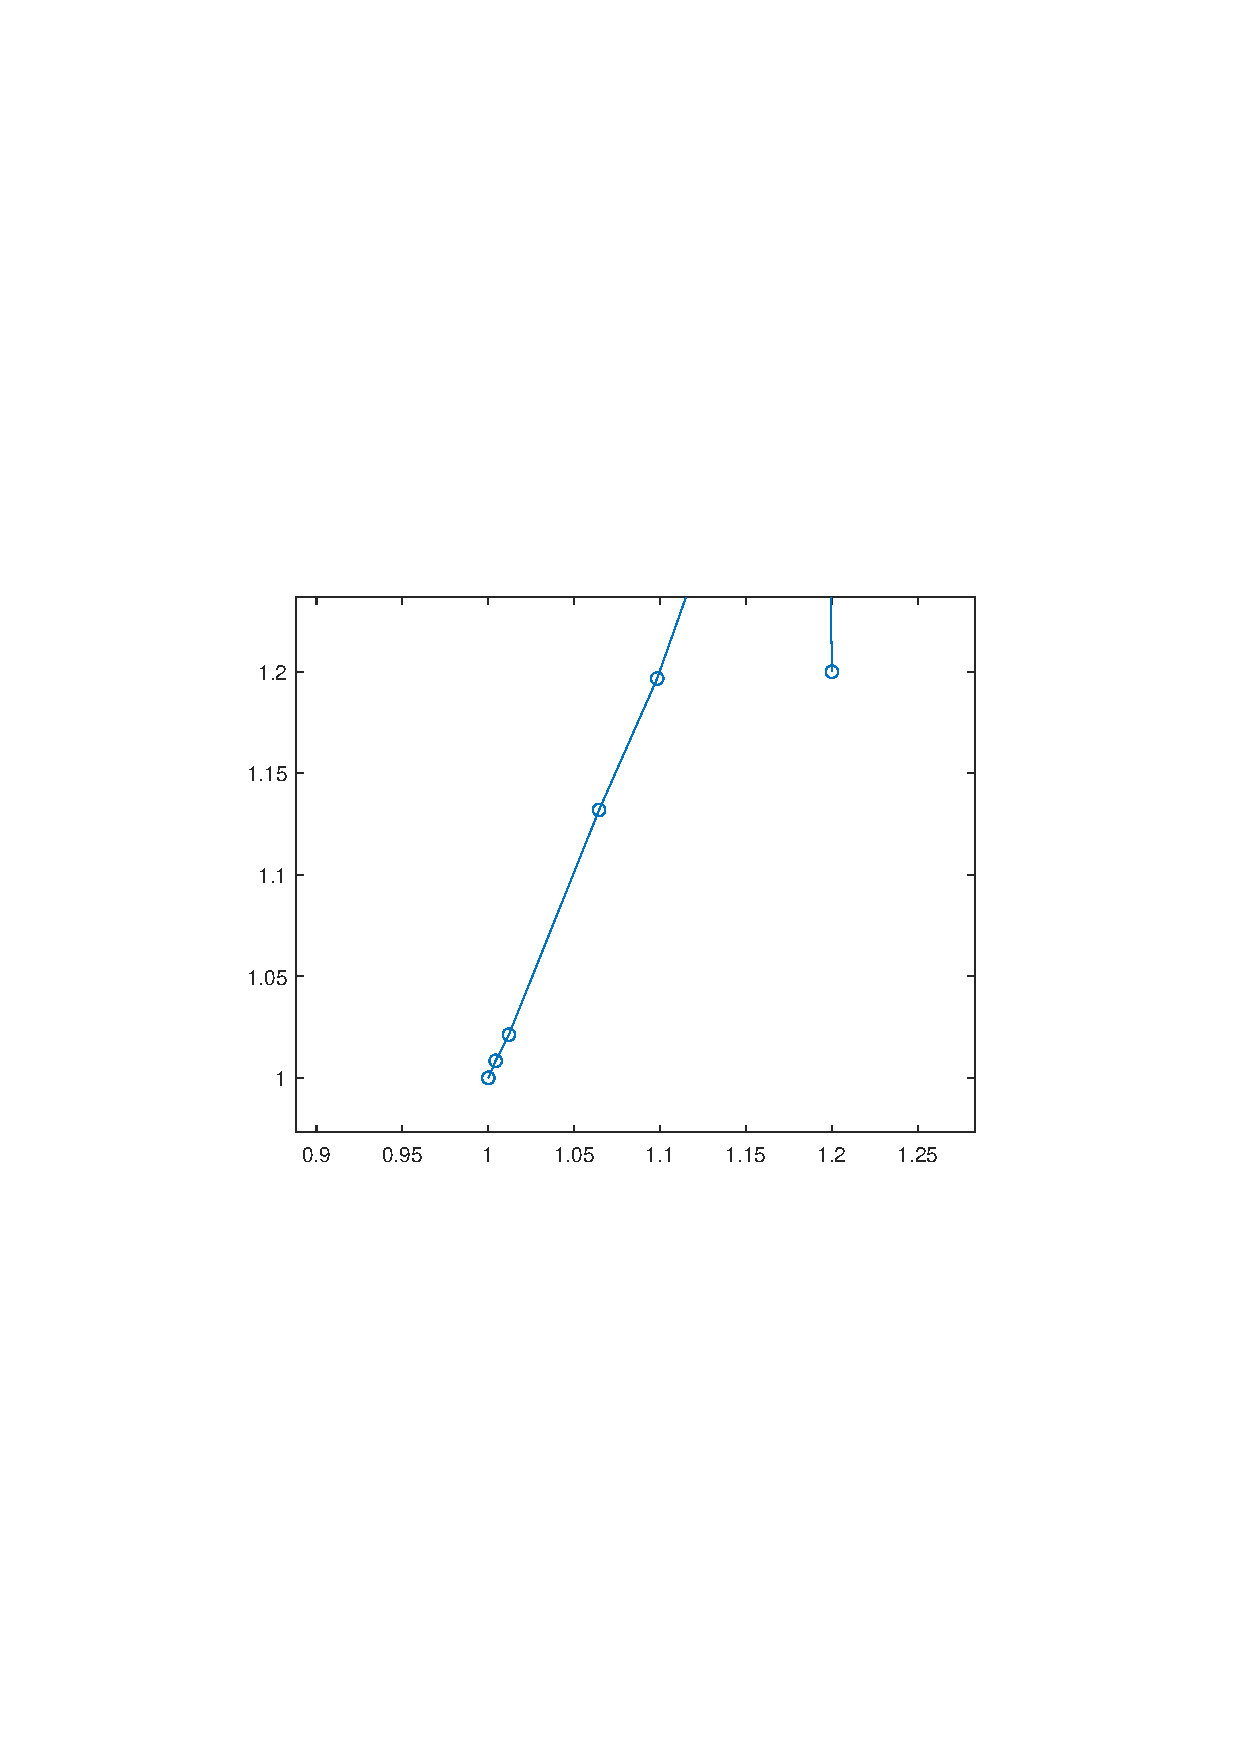
\includegraphics[width=5cm]{fig/4_33.pdf}}
\subfigure{
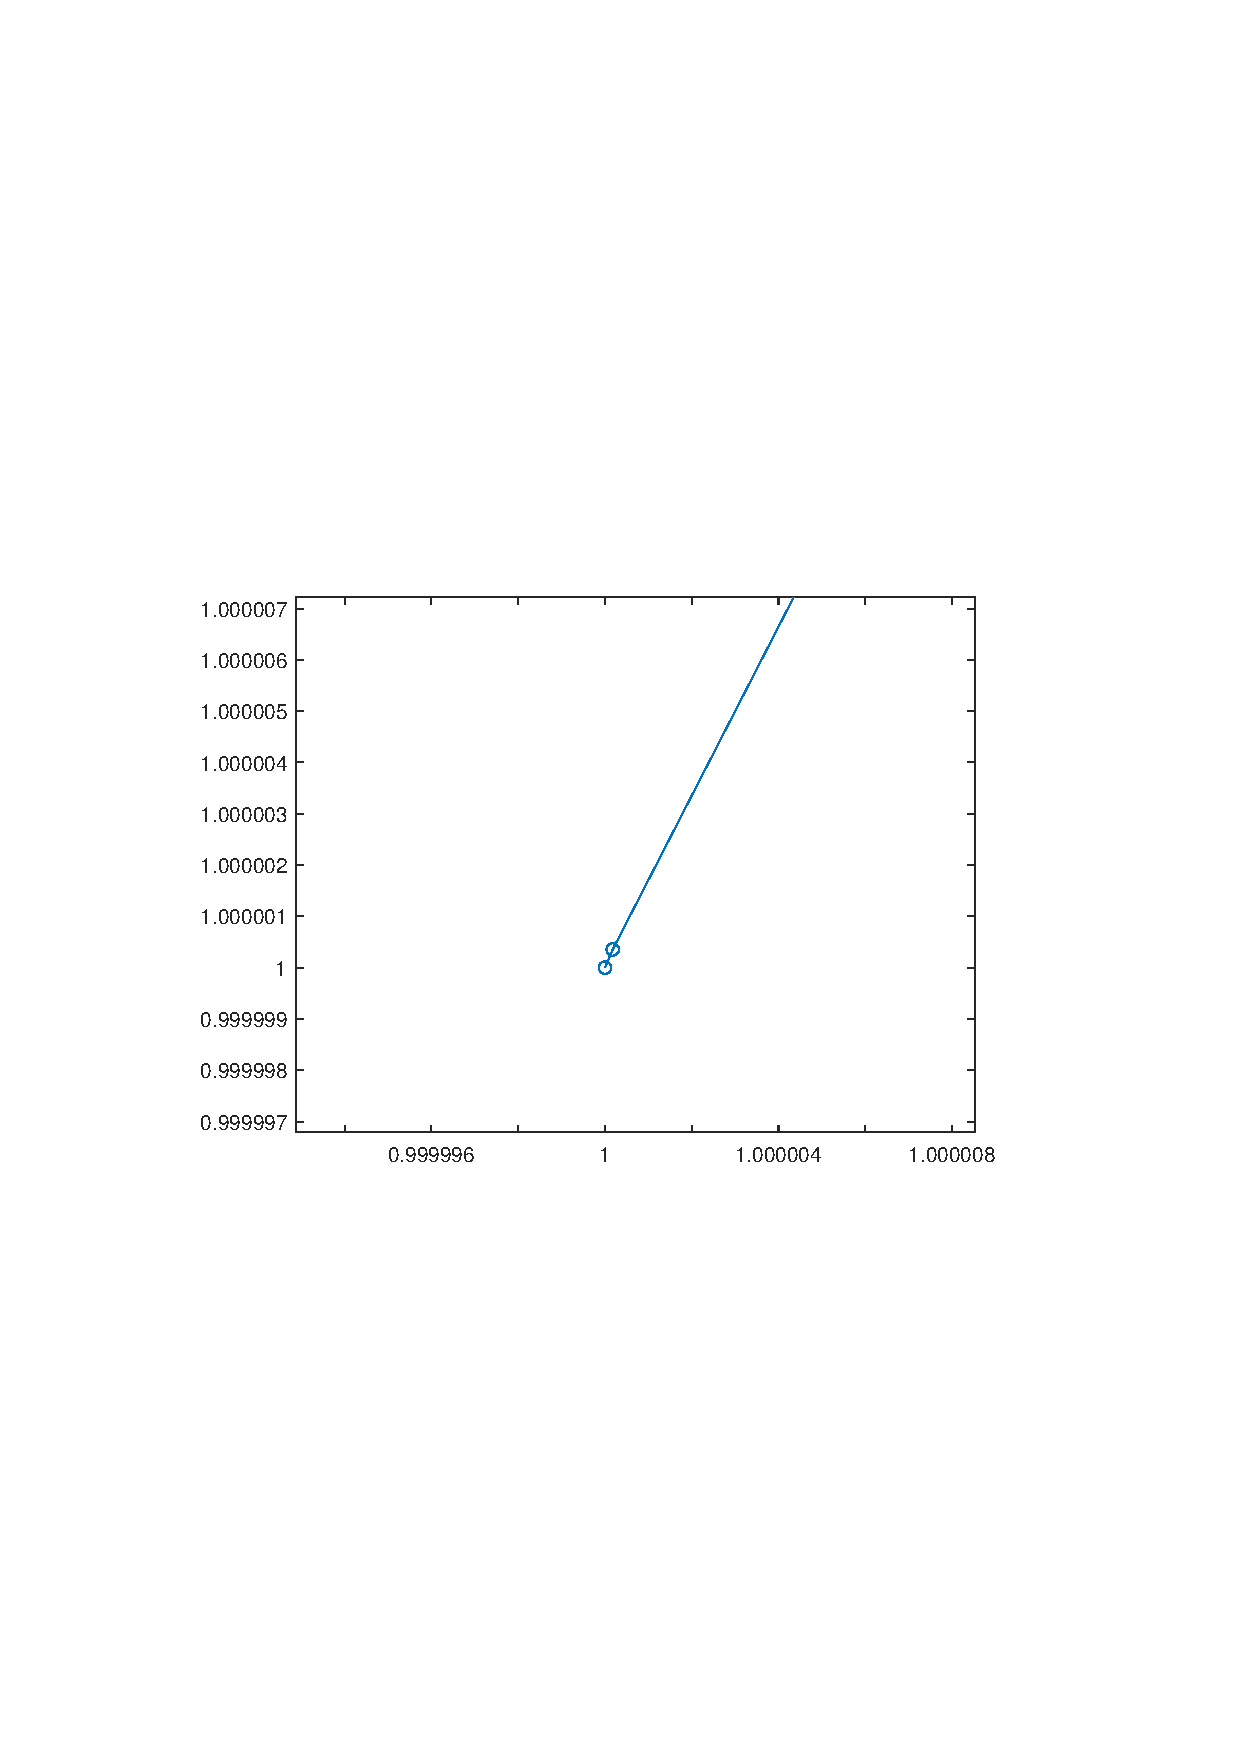
\includegraphics[width=5.3cm]{fig/4_34.pdf}}
\caption{Newton-Armijo in (1.2,1.2)}
\label{Fig.lable}
\end{figure}

\begin{lstlisting}
%Result for Newton-Armijo in (1.2,1.2)
Step[1]: x=[ 1.200000 1.200000 ] optim_fx=5.800000
Step[2]: x=[ 1.195918 1.430204 ] optim_fx=0.038384
Step[3]: x=[ 1.098284 1.196688 ] optim_fx=0.018762
Step[4]: x=[ 1.064488 1.131993 ] optim_fx=0.004289
Step[5]: x=[ 1.011992 1.021372 ] optim_fx=0.000903
Step[6]: x=[ 1.004261 1.008481 ] optim_fx=0.000019
Step[7]: x=[ 1.000050 1.000083 ] optim_fx=0.000000
Step[8]: x=[ 1.000000 1.000000 ] optim_fx=0.000000
Step[9]: x=[ 1.000000 1.000000 ] optim_fx=0.000000
%牛顿 Armijo 回溯法,,共迭代 9 步
%最优解:
x=[ 1.000000e+00 1.000000e+00 ] optim_fx=0.000000
\end{lstlisting}

\begin{figure}[H]
\centering
\subfigure{
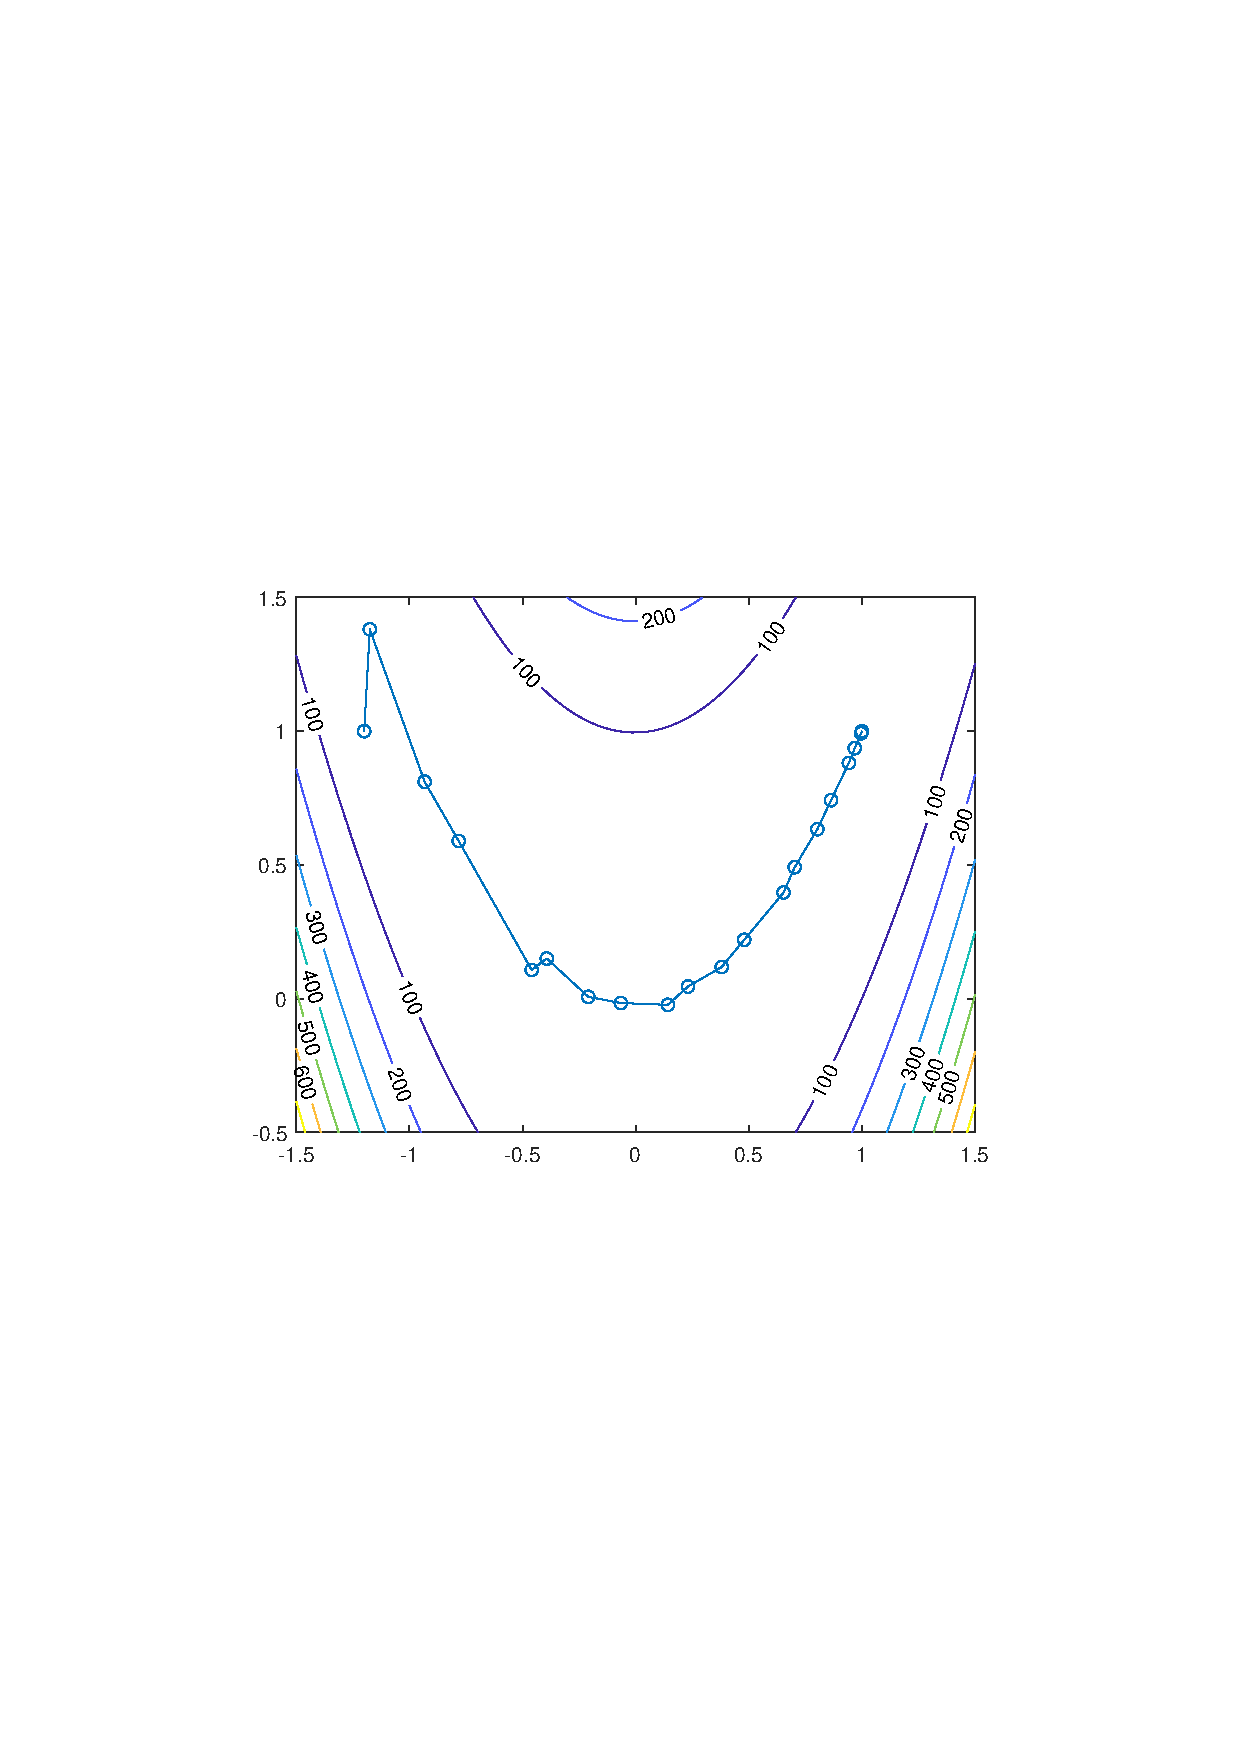
\includegraphics[width=5cm]{fig/4_41.pdf}}
\subfigure{
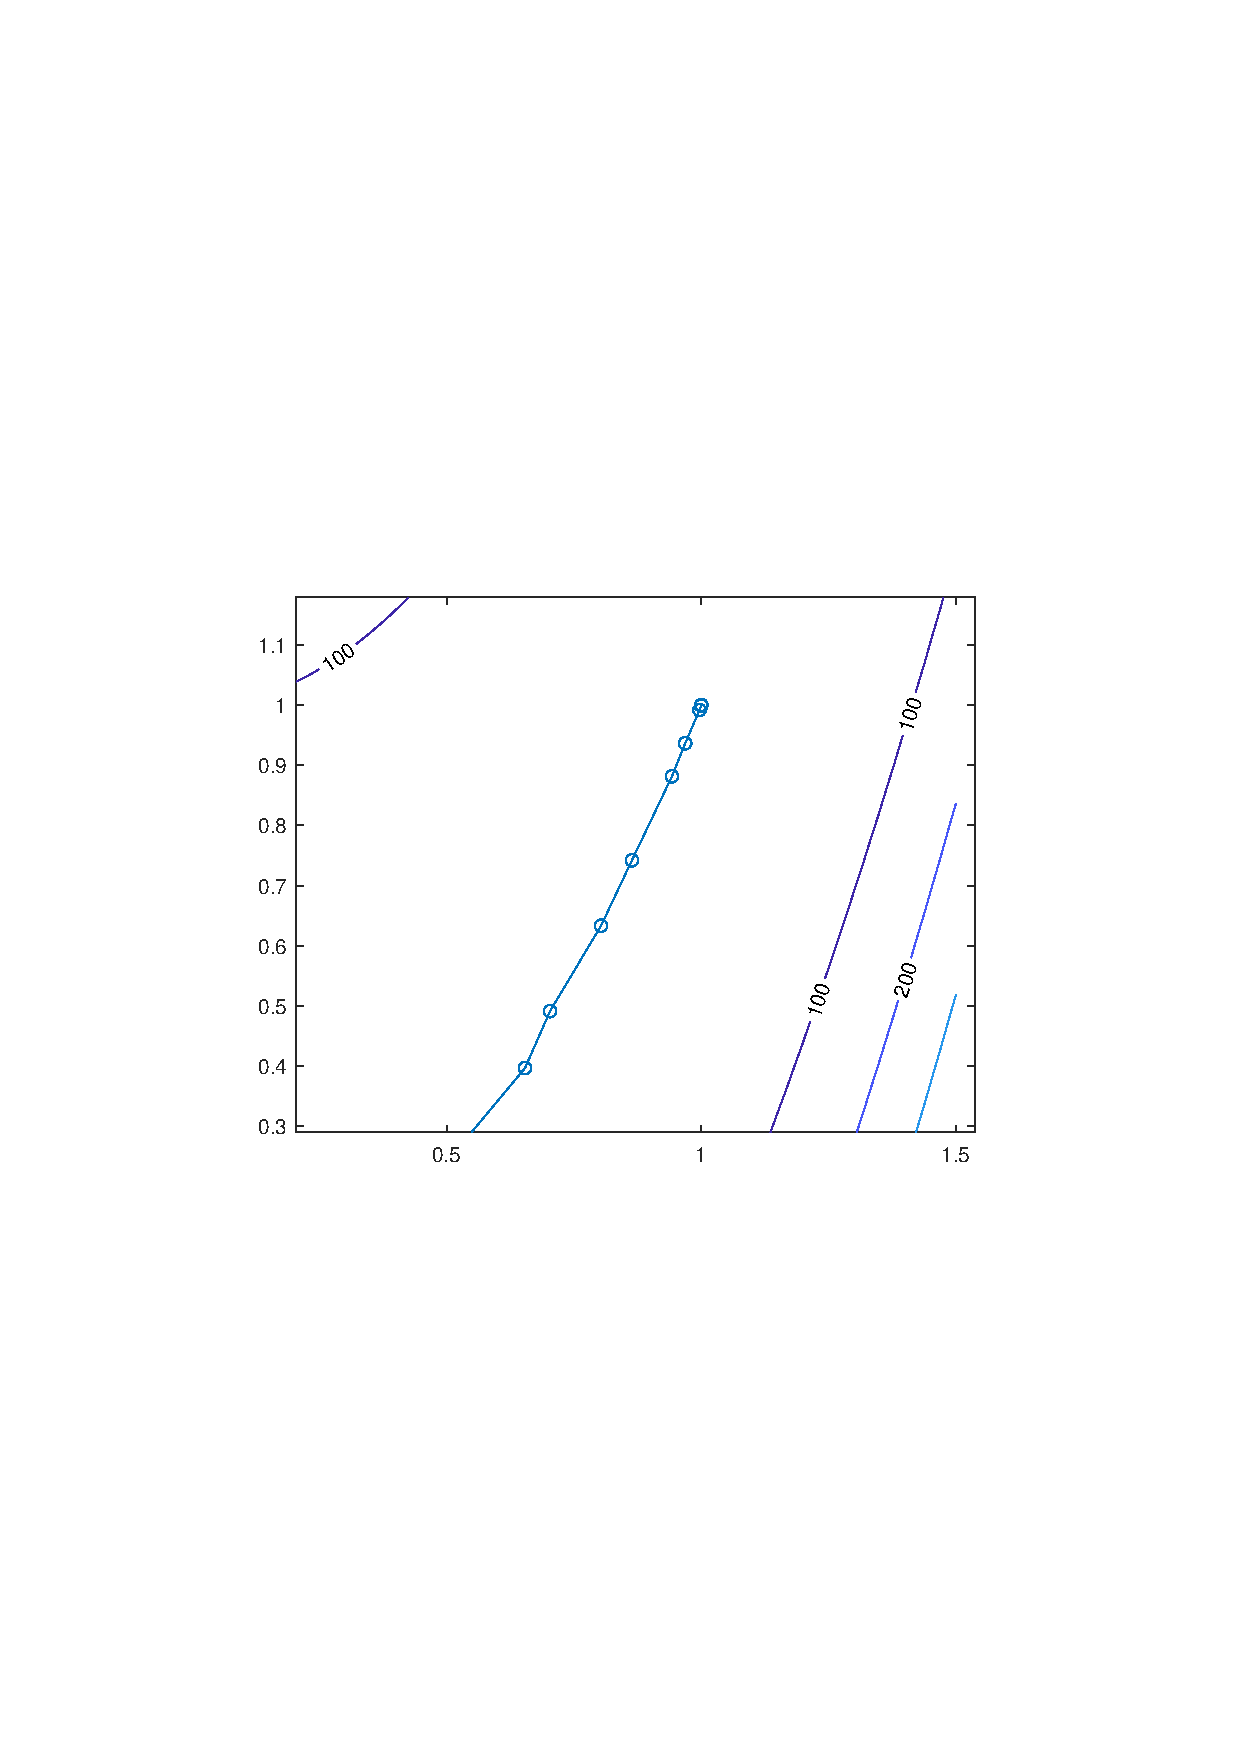
\includegraphics[width=5cm]{fig/4_42.pdf}}
\subfigure{
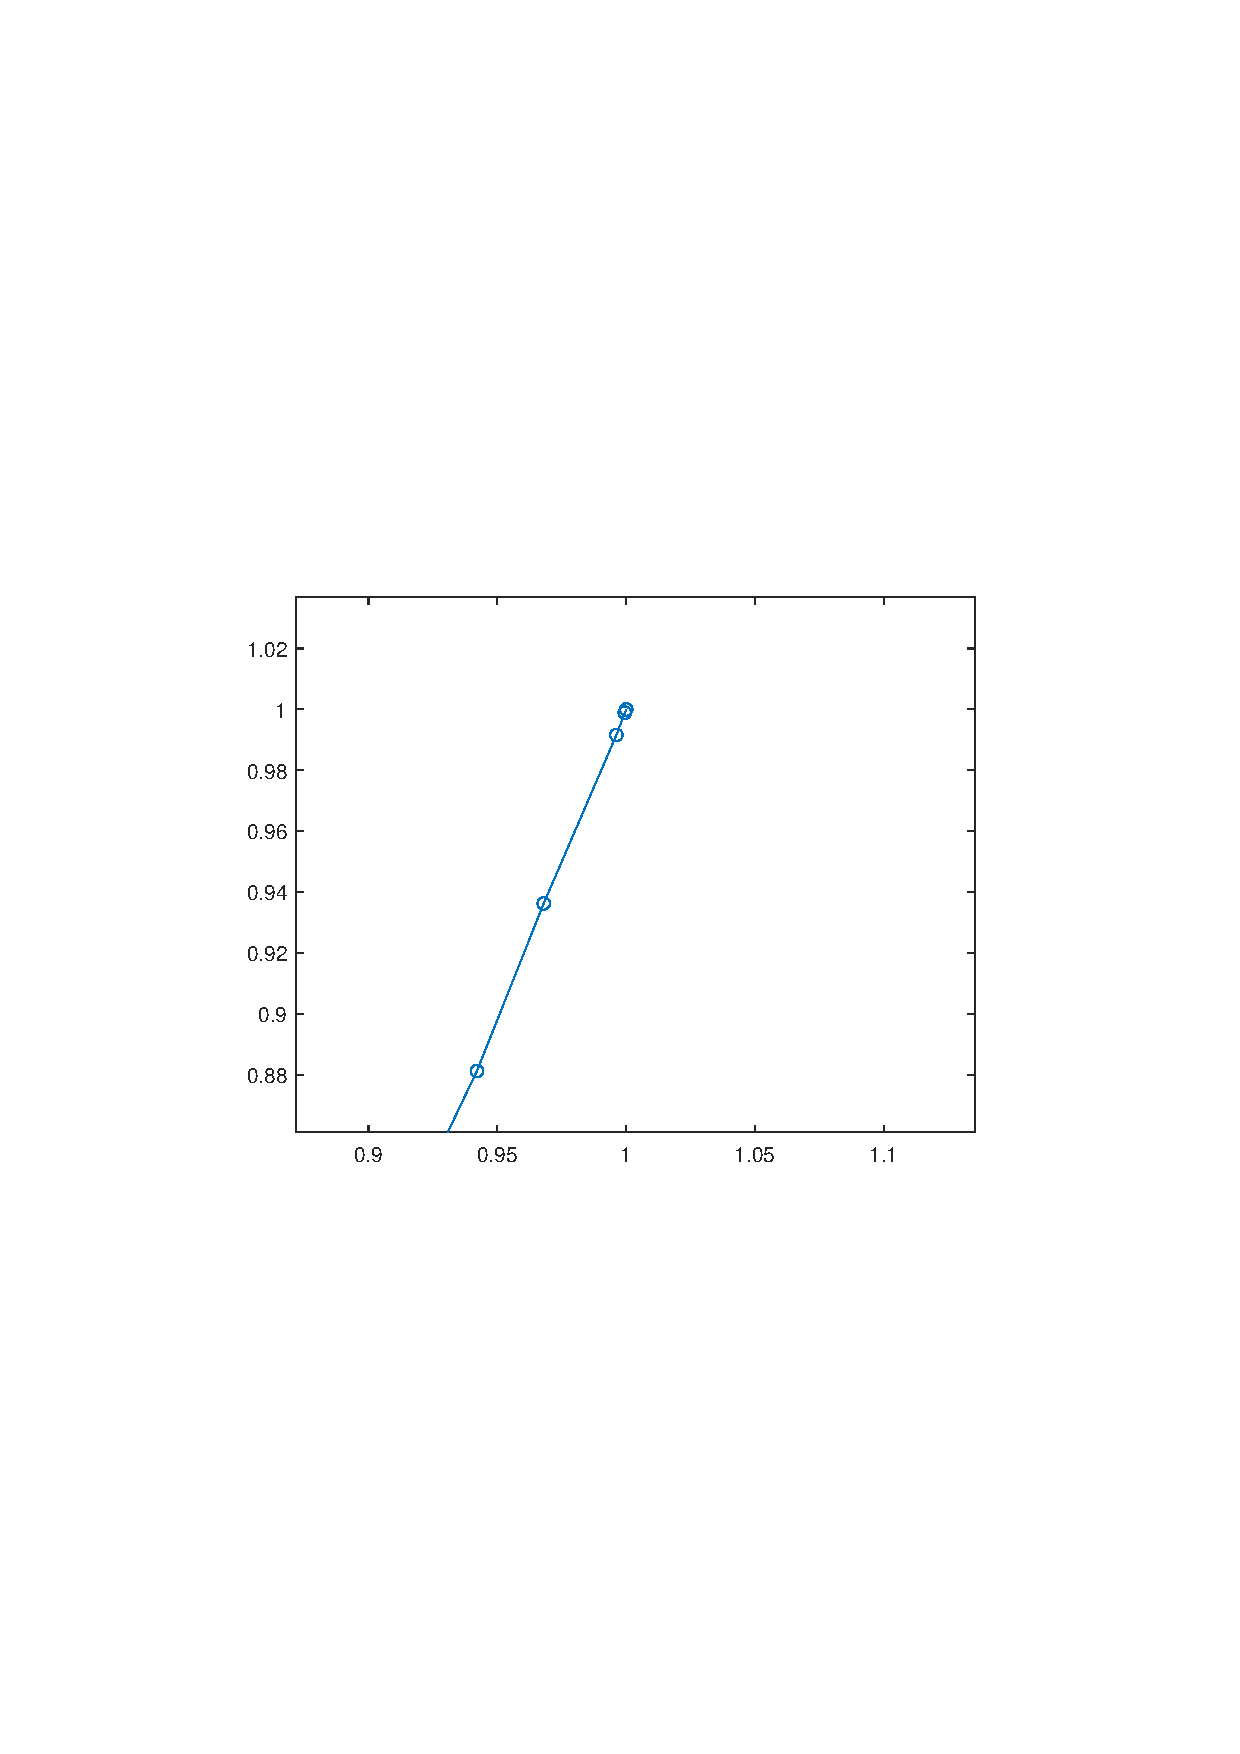
\includegraphics[width=5cm]{fig/4_43.pdf}}
\subfigure{
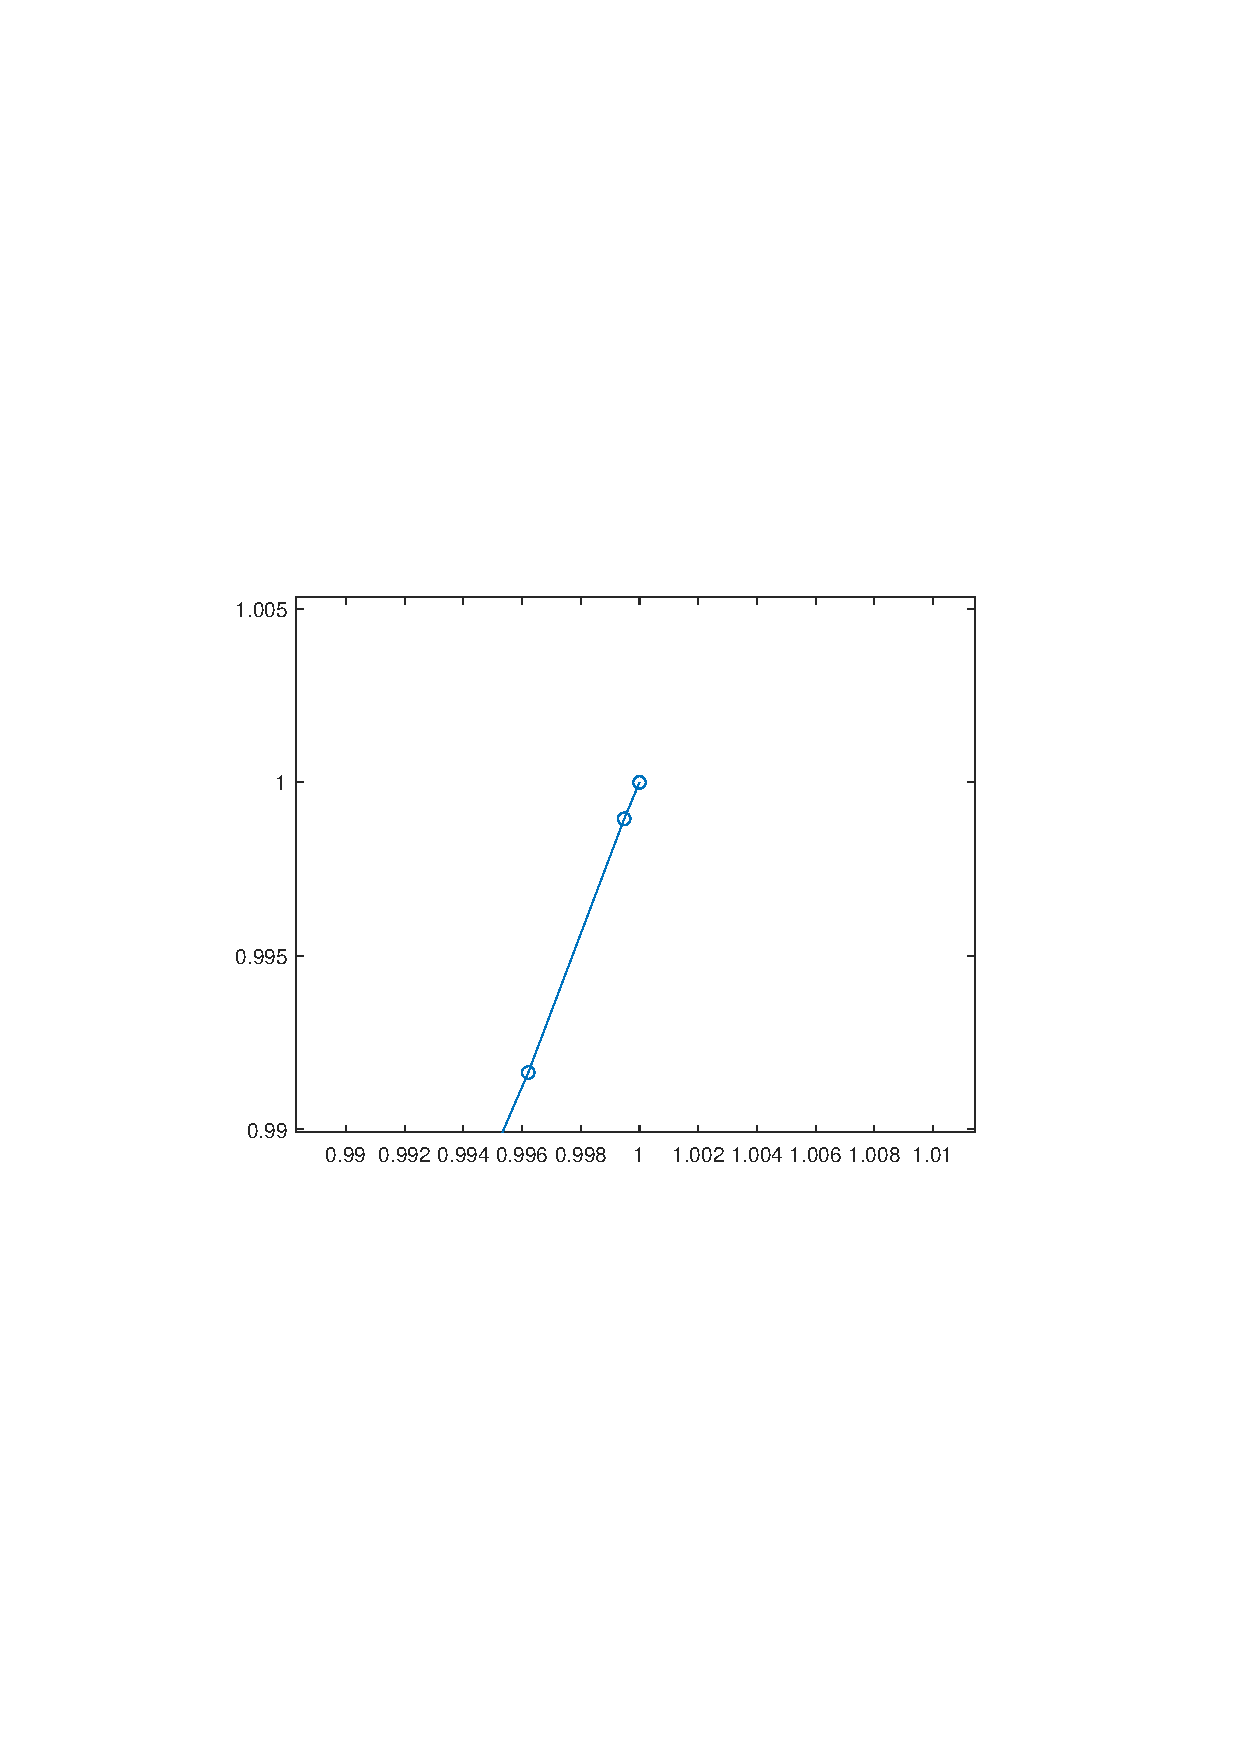
\includegraphics[width=5.3cm]{fig/4_44.pdf}}
\caption{Newton-Armijo in (-1.2,1)}
\label{Fig.lable}
\end{figure}

\begin{lstlisting}
%Result for Newton-Armijo in (-1.2,1)
Step[1]:  x=[ -1.200000 1.000000 ] optim_fx=24.200000
Step[2]:  x=[ -1.175281 1.380674 ] optim_fx=4.731884
Step[3]:  x=[ -0.932981 0.811211 ] optim_fx=4.087399
Step[4]:  x=[ -0.782540 0.589736 ] optim_fx=3.228673
Step[5]:  x=[ -0.459997 0.107563 ] optim_fx=3.213898
Step[6]:  x=[ -0.393046 0.150002 ] optim_fx=1.942585
...
...
...
Step[17]:  x=[ 0.942079 0.881336 ] optim_fx=0.007169
Step[18]:  x=[ 0.967992 0.936337 ] optim_fx=0.001070
Step[19]:  x=[ 0.996210 0.991639 ] optim_fx=0.000078
Step[20]:  x=[ 0.999479 0.998948 ] optim_fx=0.000000
Step[21]:  x=[ 0.999999 0.999998 ] optim_fx=0.000000
Step[22]:  x=[ 1.000000 1.000000 ] optim_fx=0.000000
Step[22]: x=[ 1.000000 1.000000 ] optim_fx=0.000000
%牛顿 Armijo 回溯法,,共迭代 22 步
%最优解:
x=[ 1.000000e+00 1.000000e+00 ] optim_fx=0.000000
\end{lstlisting}

\newpage
\section{Problem 5.19}
\subsection{重要数据展示}
求解对称正定的方程组$\bm{Gx}=\bm{b}$可以看作极小化二次函数\[q(\bm{x})=\dfrac{1}{2}\bm{x^TGx-b^Tx}\]
\[\bm{g}(\bm{x})=\nabla q(\bm{x})=\bm{Gx}-\bm{b}\]
其中,$\nabla^2 q(\bm{x})=\bm{G}$为Hilbert矩阵。

希尔伯特矩阵是一种系数都是单位分数的方块矩阵,希尔伯特矩阵$\bm{H}$的第$i$横行第$j$纵列的系数是$H_{{ij}}={\dfrac  {1}{i+j-1}}$

以5阶的Hilbert矩阵为例,其矩阵如下:
\[H_5=\left(\begin{array}{ccccc} 1 & \frac{1}{2} & \frac{1}{3} & \frac{1}{4} & \frac{1}{5}\\ \frac{1}{2} & \frac{1}{3} & \frac{1}{4} & \frac{1}{5} & \frac{1}{6}\\ \frac{1}{3} & \frac{1}{4} & \frac{1}{5} & \frac{1}{6} & \frac{1}{7}\\ \frac{1}{4} & \frac{1}{5} & \frac{1}{6} & \frac{1}{7} & \frac{1}{8}\\ \frac{1}{5} & \frac{1}{6} & \frac{1}{7} & \frac{1}{8} & \frac{1}{9} \end{array}\right)\]

希尔伯特矩阵是一种数学变换矩阵,正定,且高度病态(即,任何一个元素发生一点变动,整个矩阵的行列式的值和逆矩阵都会发生巨大变化),病态程度和阶数相关。

希尔伯特矩阵的一个特点就是条件数特别大,以上面的5阶Hilbert矩阵为例,当范数为$l_2$矩阵范数时,其条件数大约是$4.8\times 10^{5}$

经证明:当 $ n\rightarrow \infty$的时候,$ n\times n$的希尔伯特矩阵的条件数近似为$O((1+{\sqrt  {2}})^{{4n}}/{\sqrt  {n}})$

MATLAB中有直接生成$N$阶希尔伯特矩阵的函数:\boxed{hilb(N)}

\newpage
\subsection{算法伪代码}
\begin{algorithm}[h]  
\caption{Conjugate gradient method method for problem(5.19)}  
\begin{algorithmic}[1]  
\STATE Given $\bm{x}^{(0)}$  and $\bm{G}$
\STATE Set $\bm{g}^{(0)}=\bm{Gx}^{(0)}-\bm{b}$
\STATE Set $\bm{p}^{(0)}=-\bm{g}^{(0)},k=0$
\WHILE {$\|\bm{g}^{(k)}\|>\epsilon$}
\STATE Set $\bm{d}=\bm{G}\bm{p}^{(k)}$
\STATE Set $\alpha_k=\dfrac{{\bm{g}^{(k)}}^T\bm{g}^{(k)}}{{\bm{p}^{(k)}}^T\bm{d}}$
\STATE Set $\bm{x}^{(k+1)}=\bm{x}^{(k)}+\alpha_k\bm{p}^{(k)}$
\STATE Set $\bm{g}^{(k+1)}=\bm{g}^{(k)}+\alpha_k\bm{d}$
\STATE Set $\beta_{k+1}=\dfrac{{\bm{g}^{(k+1)}}^T\bm{g}^{(k+1)}}{{\bm{g}^{(k)}}^T{\bm{g}^{(k)}}}$
\STATE Set $\bm{p}^{(k+1)}=-\bm{g}^{(k+1)}+\beta_{k+1}\bm{p}^{(k)}$
\STATE Set $k=k+1$
\ENDWHILE
\RETURN $\bm{x}^{(k)}$ as $\bm{x}^{\star}$
\end{algorithmic}  
\end{algorithm}

\subsection{迭代结果展示}
求解不同阶数Hilbert矩阵的迭代次数列成表格如下:

\begin{table}[htbp]
  \centering
  \caption{迭代次数}
    \begin{tabular}{ccccc}
\toprule
\textbf{n} &5& 8& 12 & 20 \\
	\midrule
\textbf{step}&6   & 19  & 35  & 66 \\
\bottomrule
    \end{tabular}
\end{table}

\begin{figure}[H]
\centering
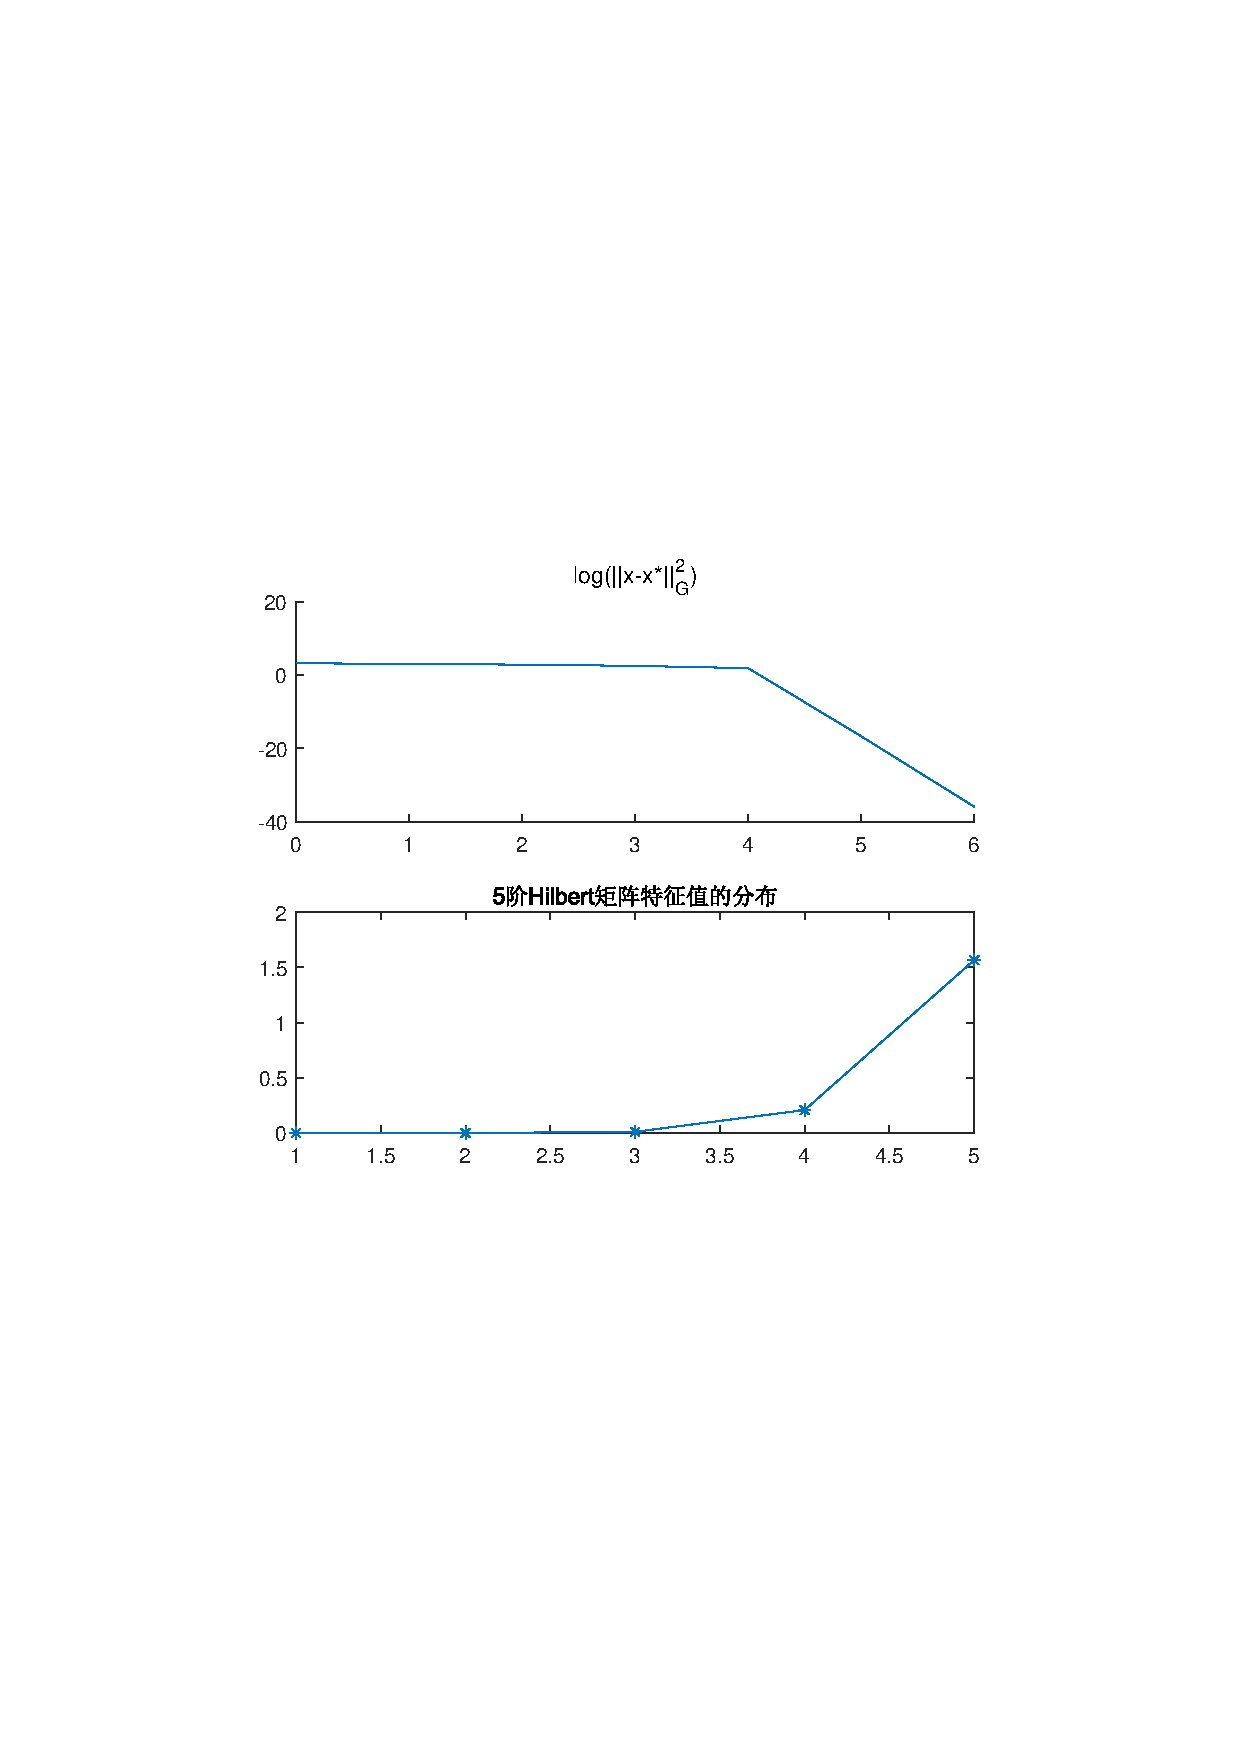
\includegraphics[width=10.5cm]{fig/5_1.pdf}
%\caption{5阶Hilbert矩阵}
\end{figure}

\begin{figure}[H]
\centering
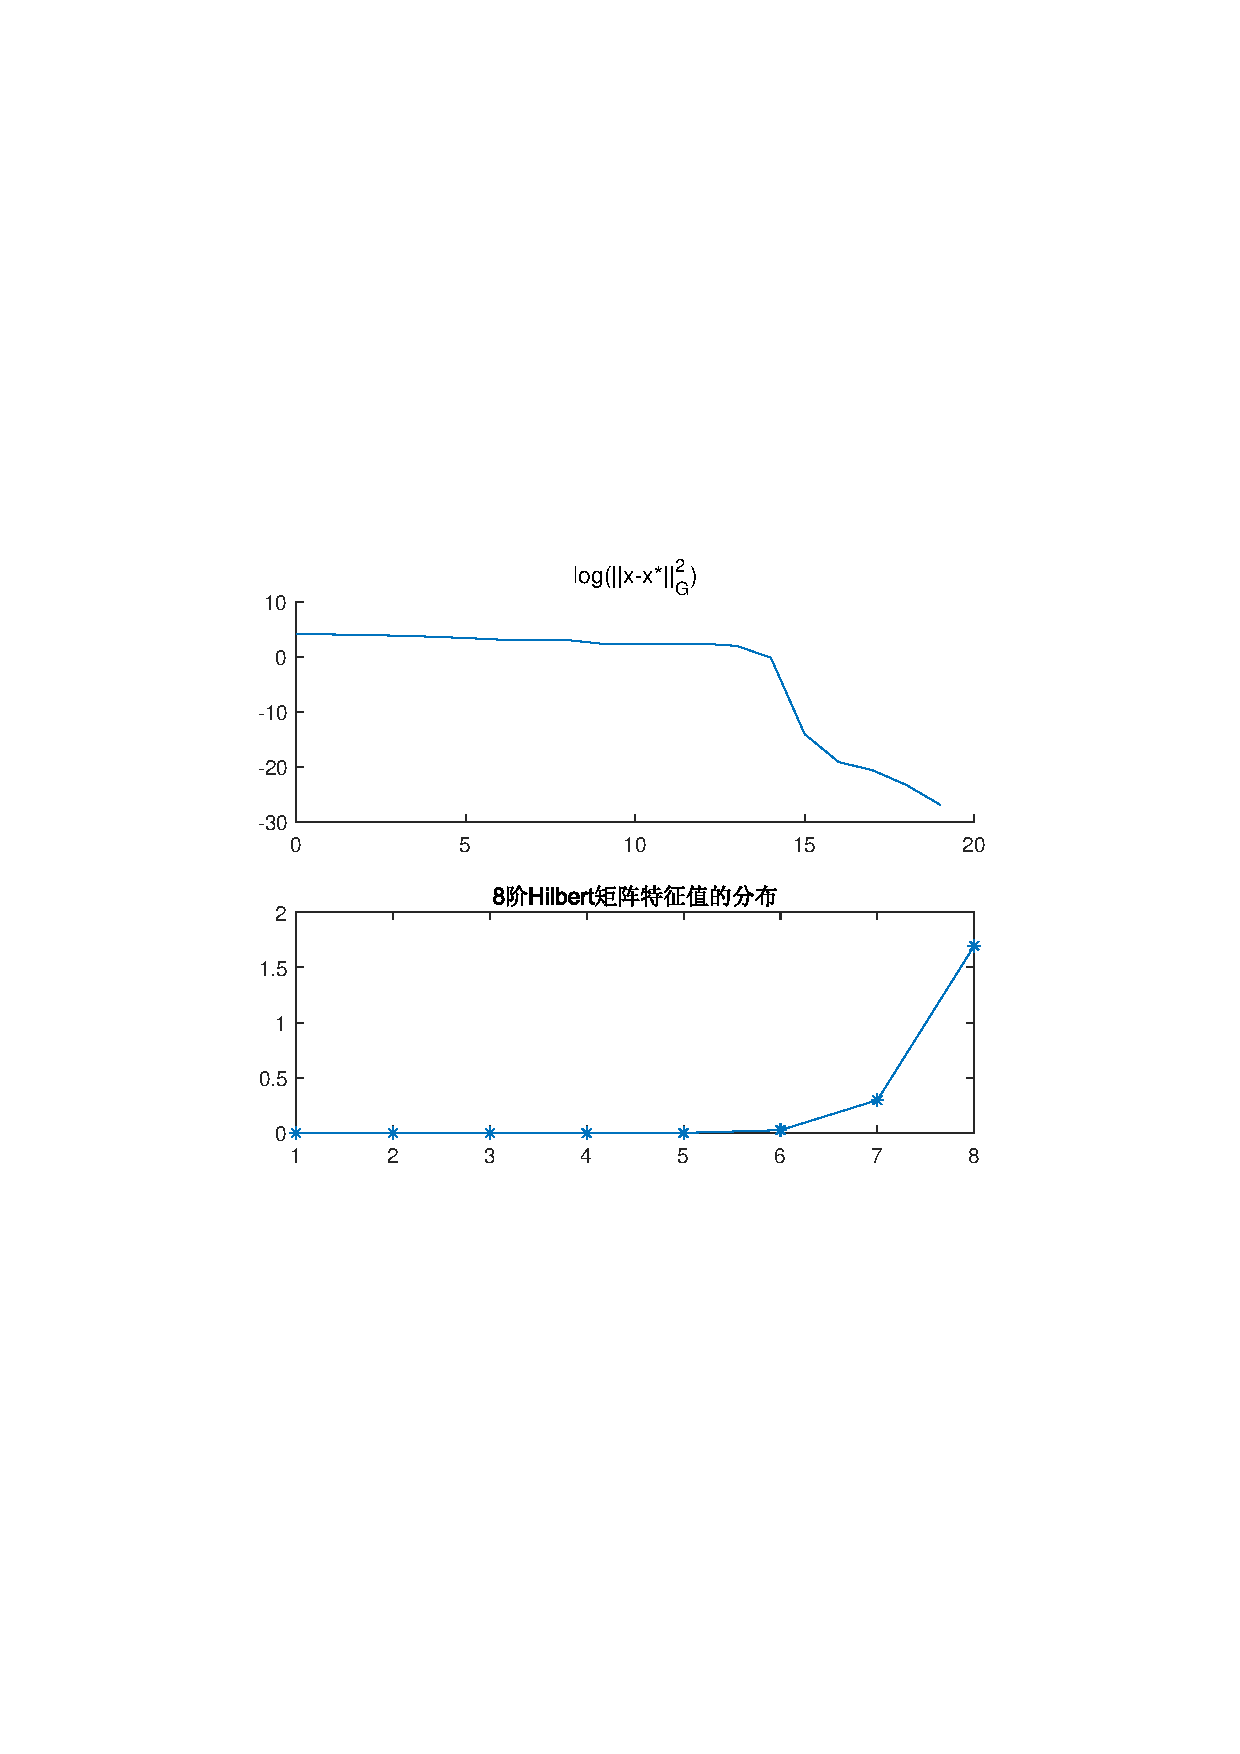
\includegraphics[width=10.5cm]{fig/5_2.pdf}
%\caption{8阶Hilbert矩阵}
\end{figure}

\begin{figure}[H]
\centering
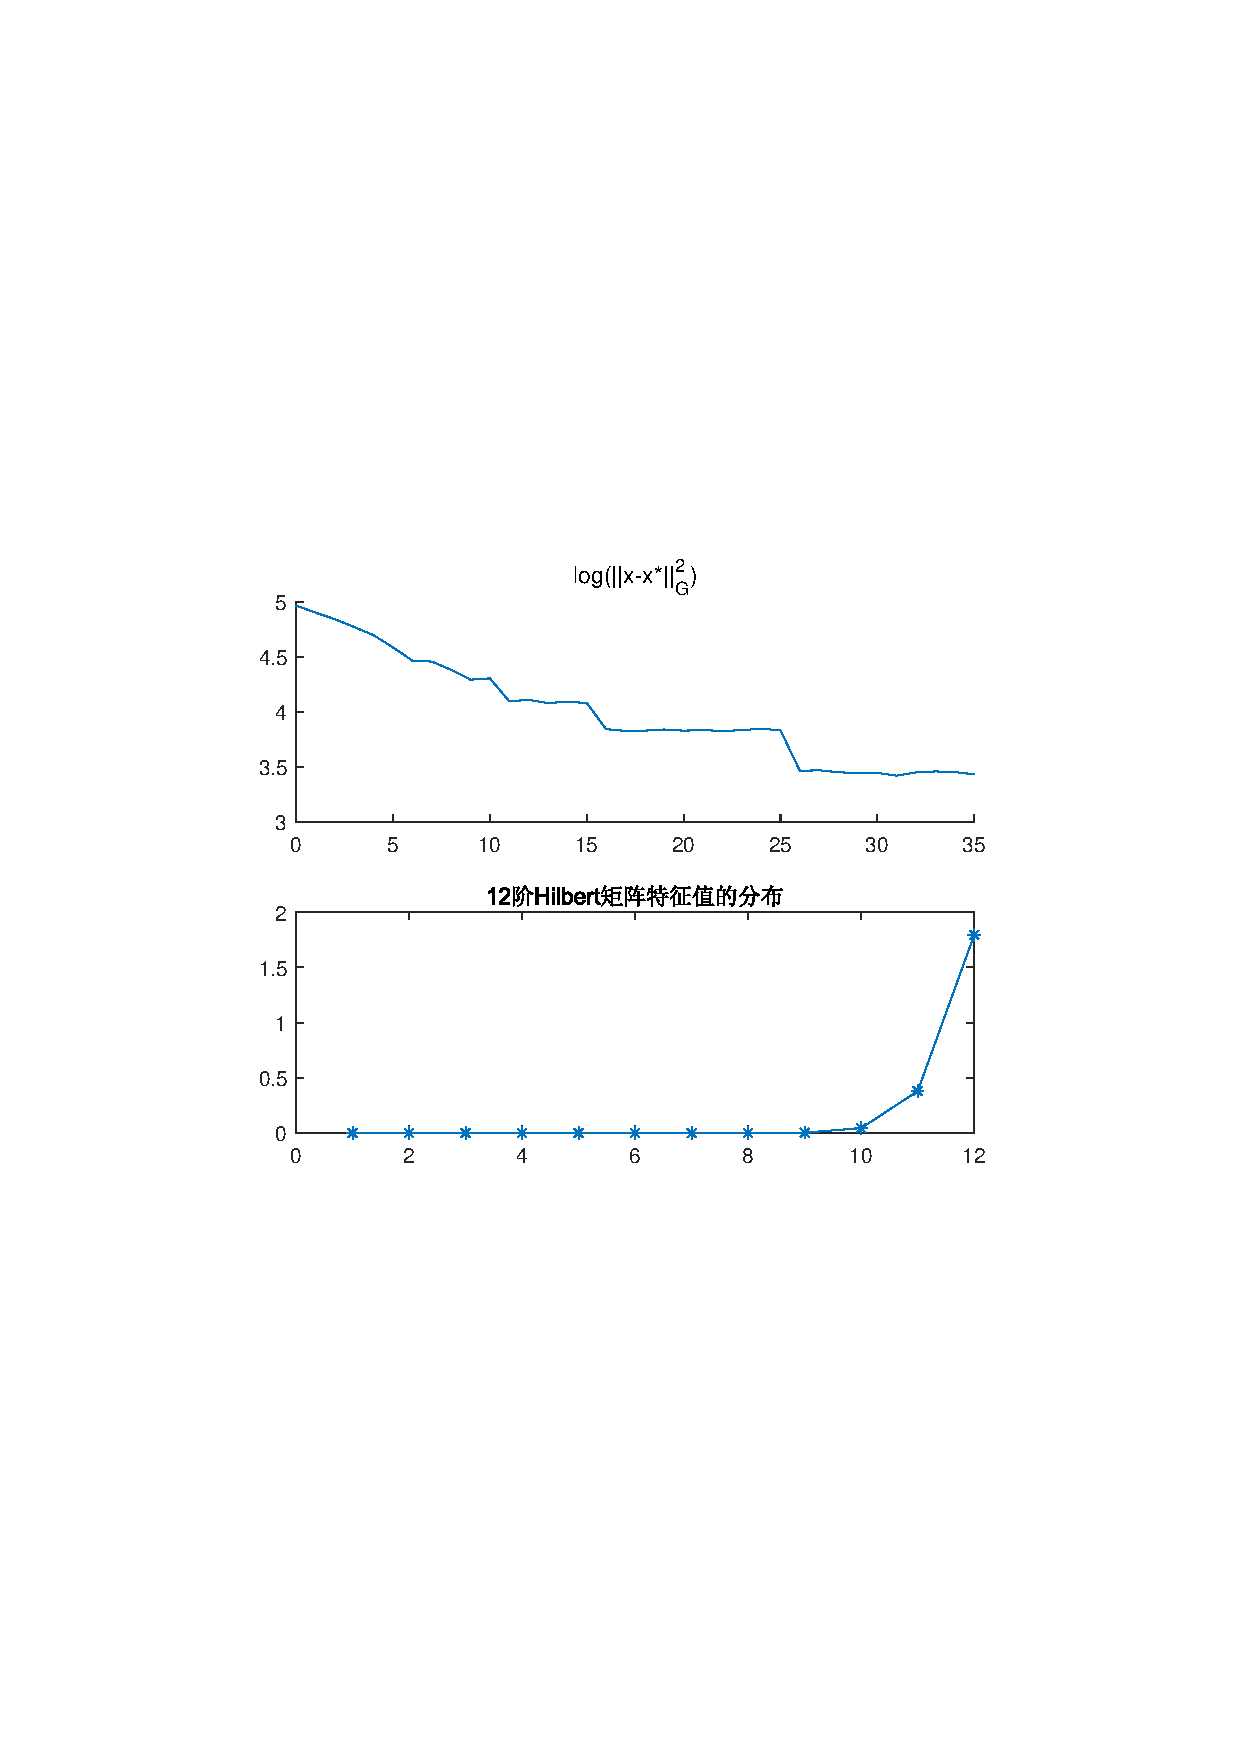
\includegraphics[width=10.5cm]{fig/5_3.pdf}%\caption{12阶Hilbert矩阵}
\end{figure}

\begin{figure}[H]
\centering
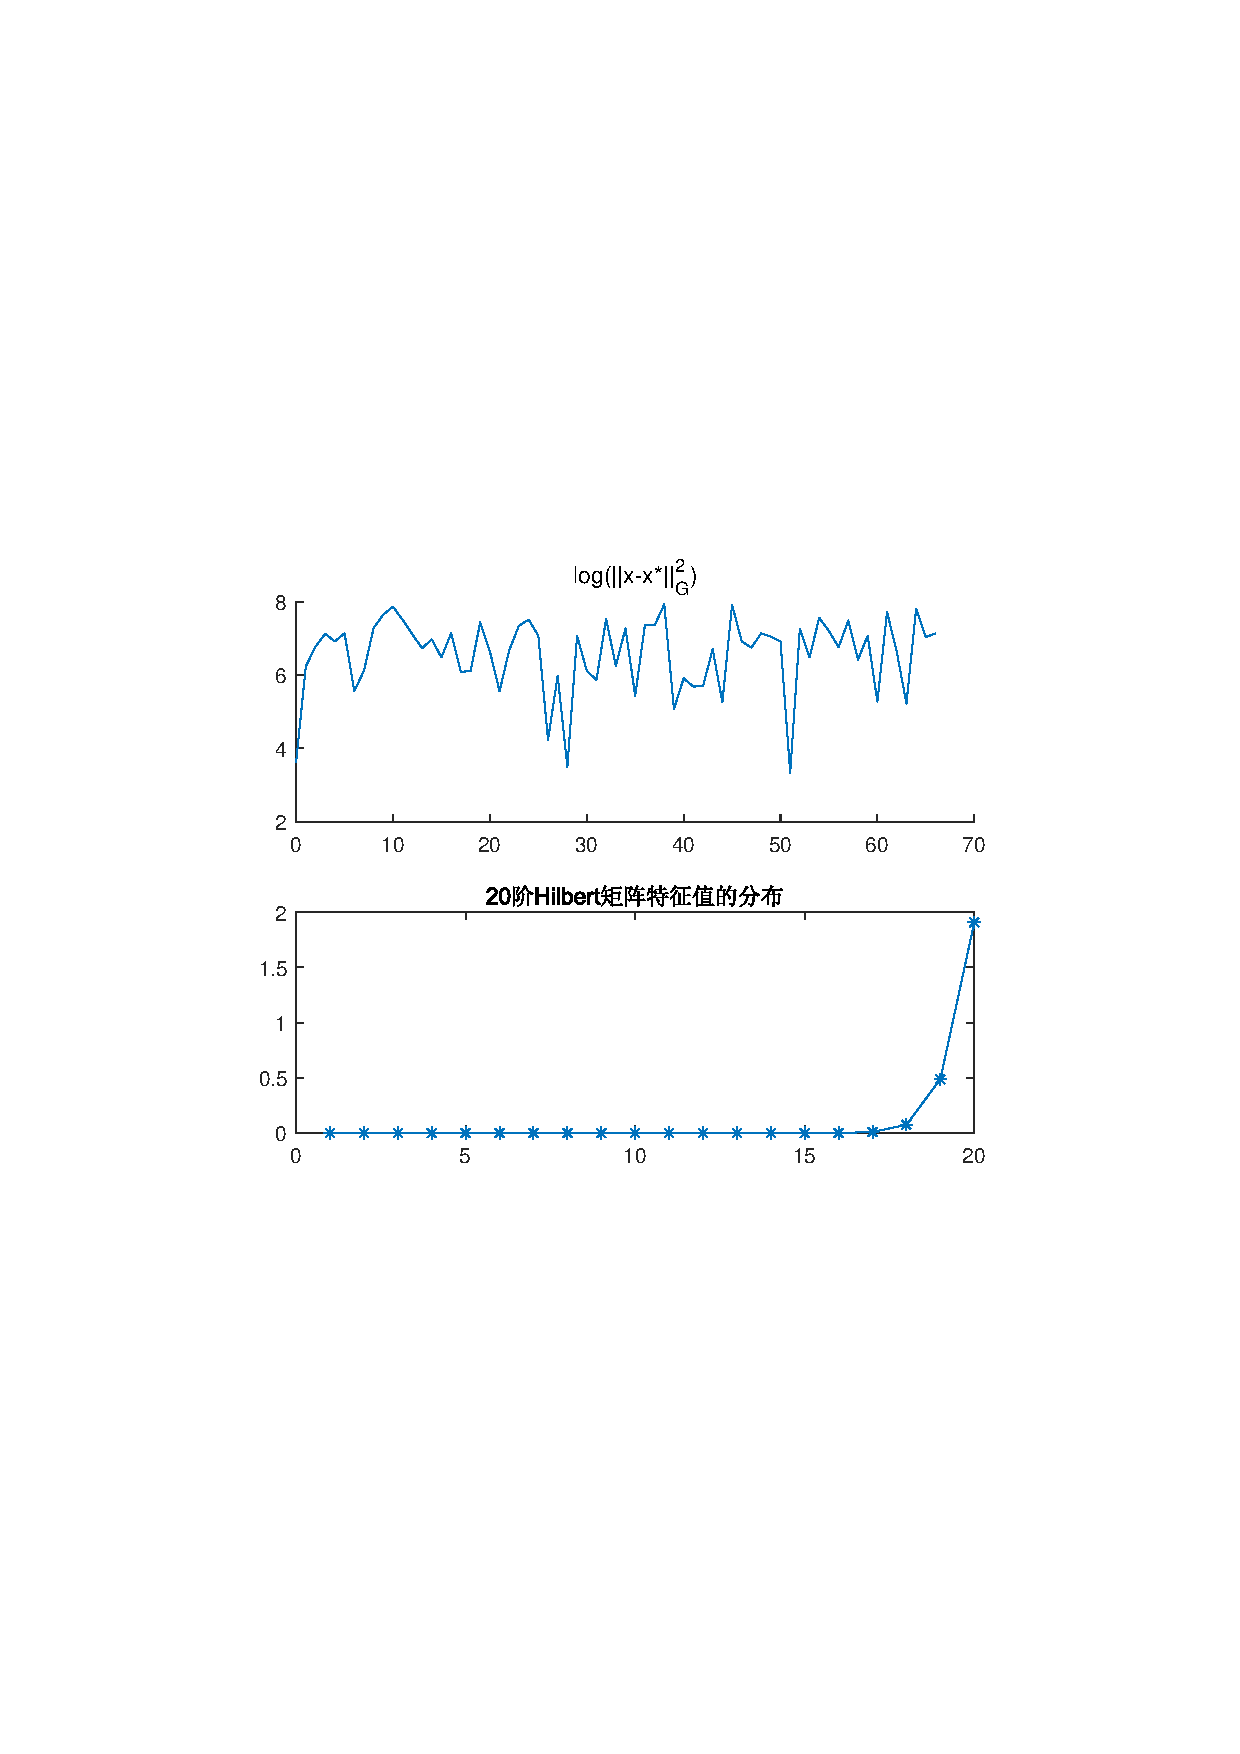
\includegraphics[width=10.5cm]{fig/5_4.pdf}
%\caption{20阶Hilbert矩阵}
\end{figure}

\subsection{总结分析}
首先我们通过一个小程序考察一下Hilbert矩阵的病态性质:

\begin{lstlisting}
N=20;
G=random('unif',0,1,[N N]);
G1=inv(G);
I=eye(N);
norm(G*G1-I)

%ans =
%
%  2.9348e-14
\end{lstlisting}

先生成一个$20\times 20$的随机矩阵,然后用MATLAB自带的求逆函数inv()求逆,然后将原矩阵与其逆相乘再减去单位阵,之后求矩阵范数,求得结果为2.9348e-14,可见MATLAB自带的求逆函数在面对一般问题时还是比较精确的。

\begin{lstlisting}
N=20;
H=hilb(N);
H_inv=inv(H);
I=eye(N);
norm(H*H_inv-I)

%ans =
%
%  33.8220
\end{lstlisting}



然后我们对Hilbert矩阵进行相同操作,结果为33.8220,远远大于上面那个结果,足以见Hilbert矩阵的高度病态性质。

另外,我们由书本知识可以知道:共轭梯度法与特征值的分布有关,当特征值分布较密集时,相同步数迭代精度更高。所以我们可以对Hilbert矩阵进行预处理,降低其条件数。

嗯,那如何对Hilbert矩阵进行预处理呢?我在网上经过不懈的搜索,终于在Alfi Quarteroni的\emph{Scientifi Computing with MATLAB and Octave}中找到这么一个题目(见图\ref{exam}),题目中点出可以用Hilbert矩阵对角元素构建一个对角矩阵,作为预处理矩阵。

\begin{figure}[H]
\centering
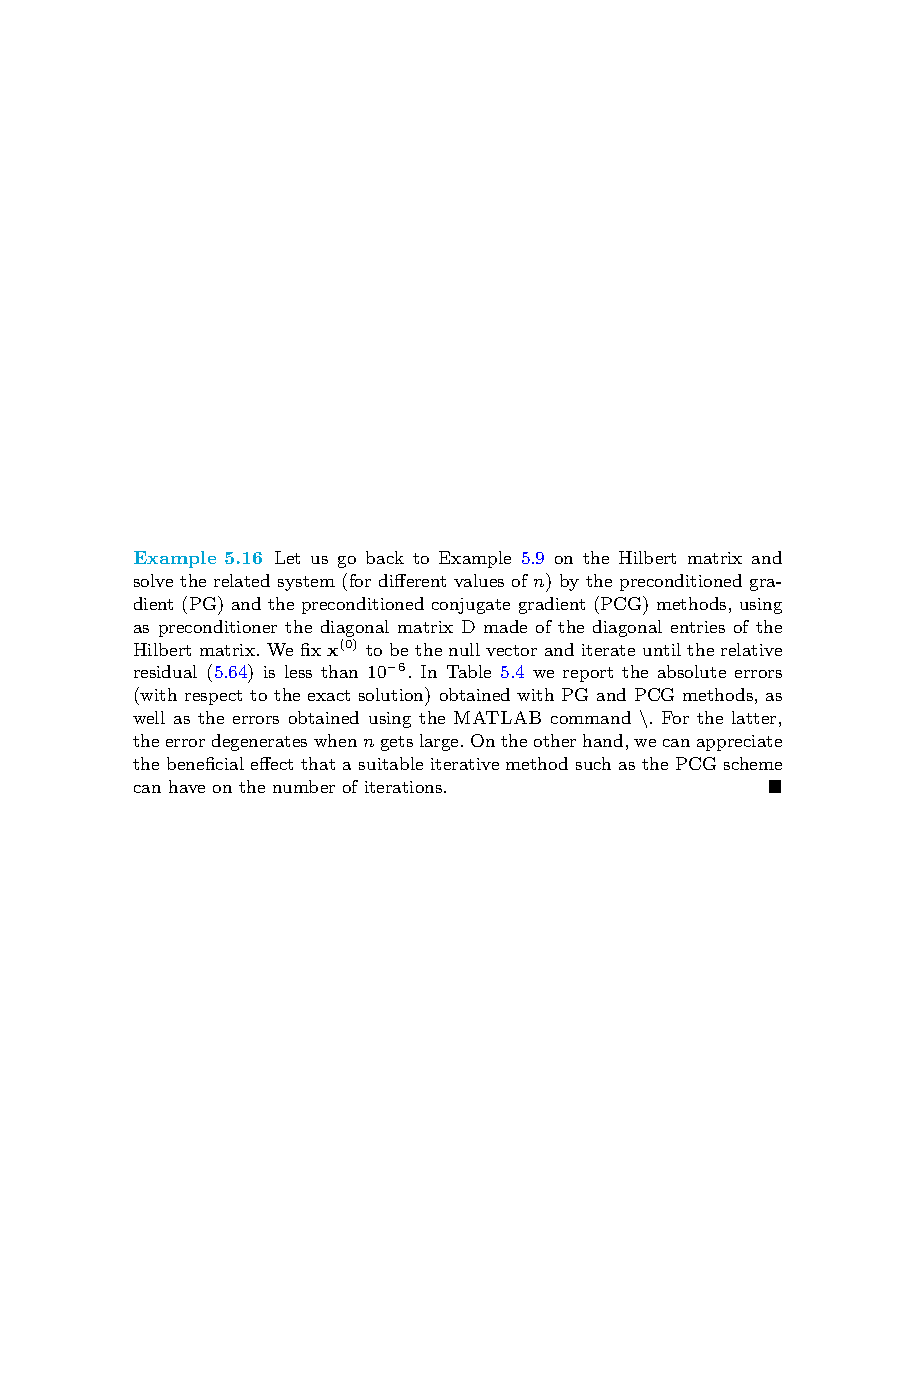
\includegraphics[width=12cm]{fig/5_5.pdf}
\caption{从书上摘的题}
\label{exam}
\end{figure}

也就是说,设$C$是由$G$的对角线元素开方构成的对角矩阵,令$\hat{G}=C^{-T}GC^{-1},\quad \hat{x}=Cx$,经过变换可调整为$M^{-1}Gx=M^{-1}b$,其中$M=C^TC$,即由$G$对角线元素构成的对角阵。

经过这么一番预处理后,不难看出不难看出该
矩阵仍然是对称正定矩阵,而且其对角元素全为 1.

那么我就使用书上的预处理共轭梯度法首先对$N=20$的Hilbert矩阵进行检验:

\begin{figure}[H]
\centering
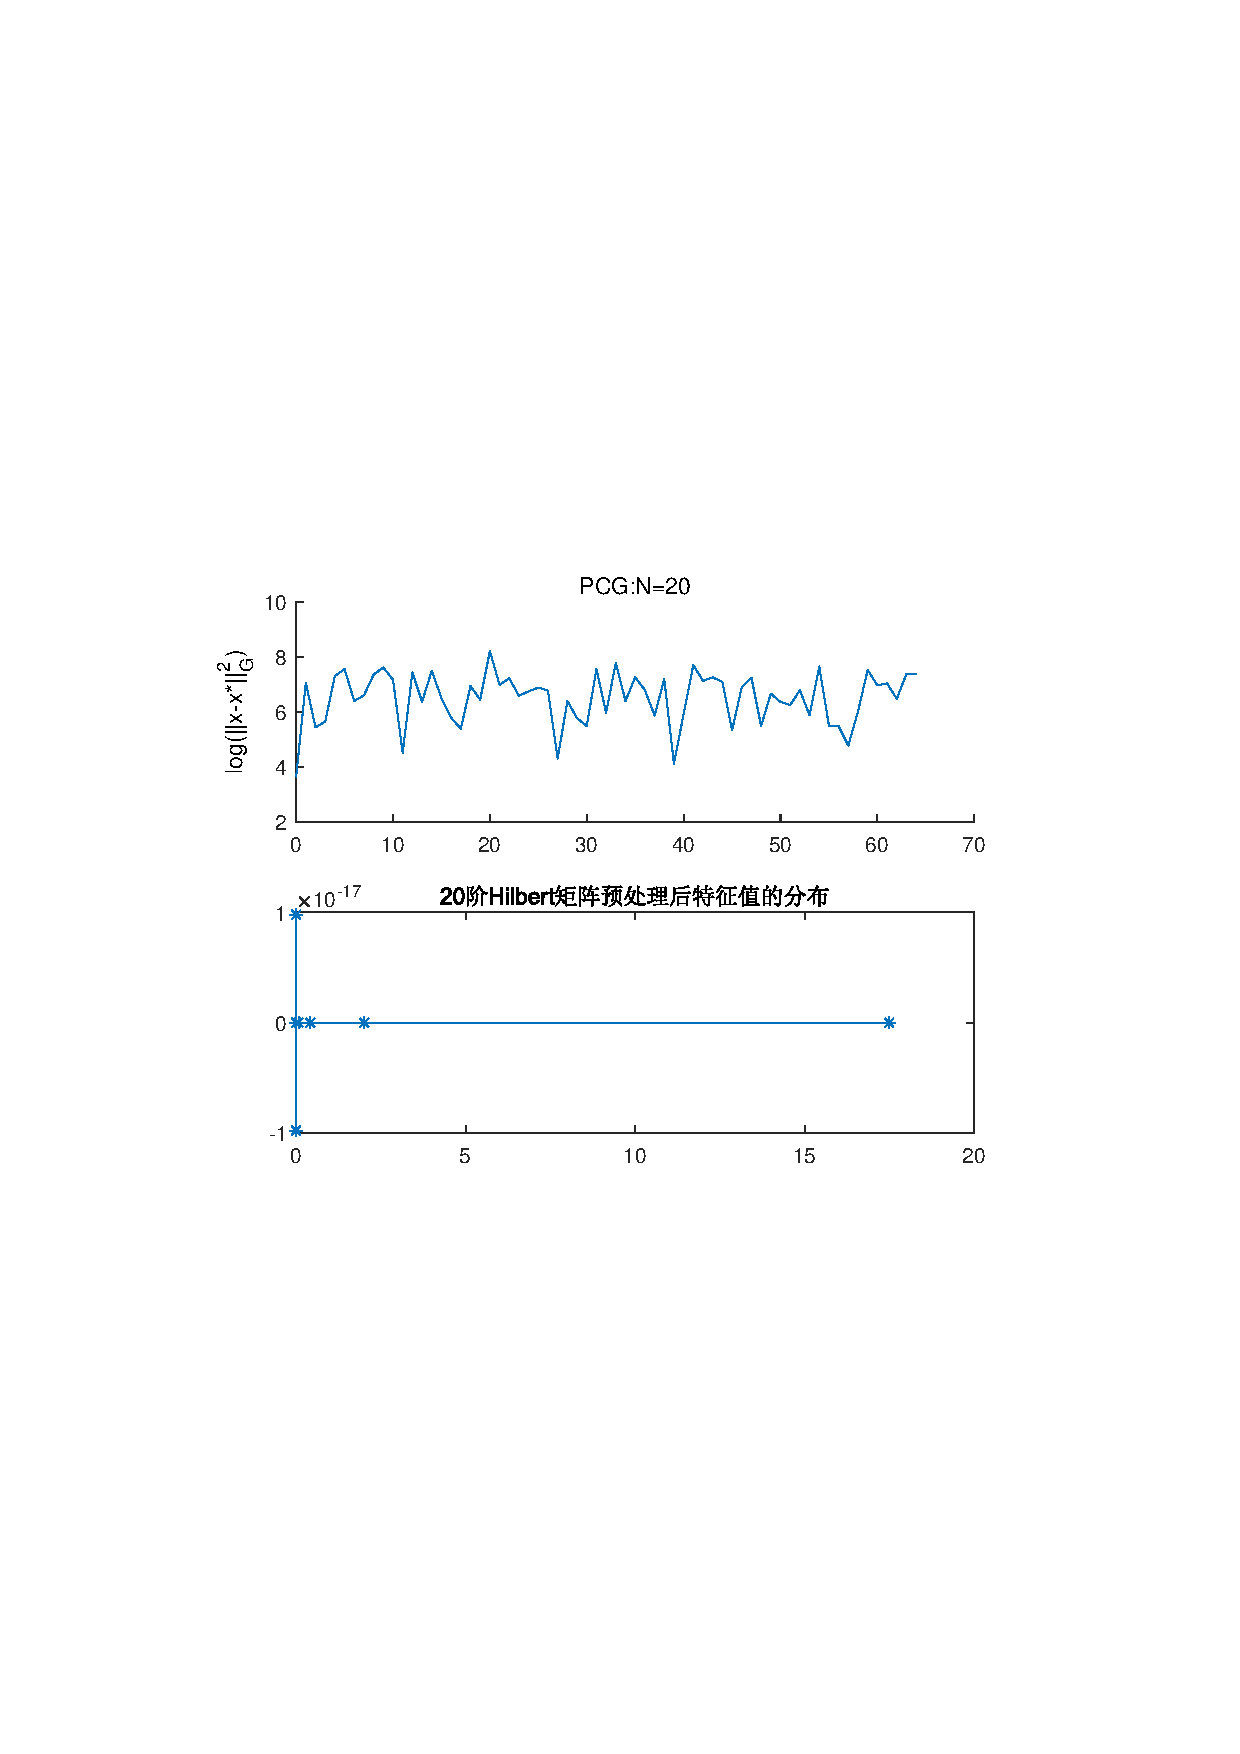
\includegraphics[width=11cm]{fig/5_7.pdf}
\end{figure}

可见这个预处理确实把特征值都聚集到一起了,但是迭代次数却为65次,仅仅比之前减少了一步,优化不太明显,这令我非常困惑,于是我改变终止精度进行测试,结果如下:

\begin{table}[htbp]
  \centering
  \caption{不同精度下迭代次数的比较$(N=20)$}
    \begin{tabular}{ccccc}
\toprule
{Error} &$10^{-6}$&$10^{-7}$& $10^{-8}$ \\
	\midrule
{Steps of CG}&66&121   & 520  \\
{Steps of PCG}&65&115   & 314 \\
\bottomrule
    \end{tabular}
\end{table}

可见在精度要求较低的情况下,两者的相差并不明显。

然后我试着将$N$调到100,观察其迭代情况,发现在精度较低时,PCG法所迭代的次数有时候甚至比CG法还要多,但在精度要求达$10^{-8}$ 时,CG法无论如何迭代都无法满足精度要求,而PCG略胜一筹,精度高出了一个数量级,且迭代次数更少。

\begin{table}[htbp]
  \centering
  \caption{不同精度下迭代次数的比较$(N=100)$}
    \begin{tabular}{ccccccc}
\toprule
{Error} &		$10^{-3}$	&		$10^{-4}$		&		$10^{-5}$		&$10^{-6}$		&		$10^{-7}$		& 	$10^{-8}$ \\
	\midrule
{Steps of CG}&12&	25&	47&175&748  & 2132(error=1.132e-08)  \\
{Steps of PCG}&15&	27&	65&111&756   & 1686(error=9.683e-09)\\
\bottomrule
    \end{tabular}
\end{table}


此外,该书上还列举了梯度下降法(PG)和预处理共轭梯度法(PCG)在求解该问题上的比较,我认为比较有借鉴意义,贴在下面:
\begin{figure}[H]
\centering
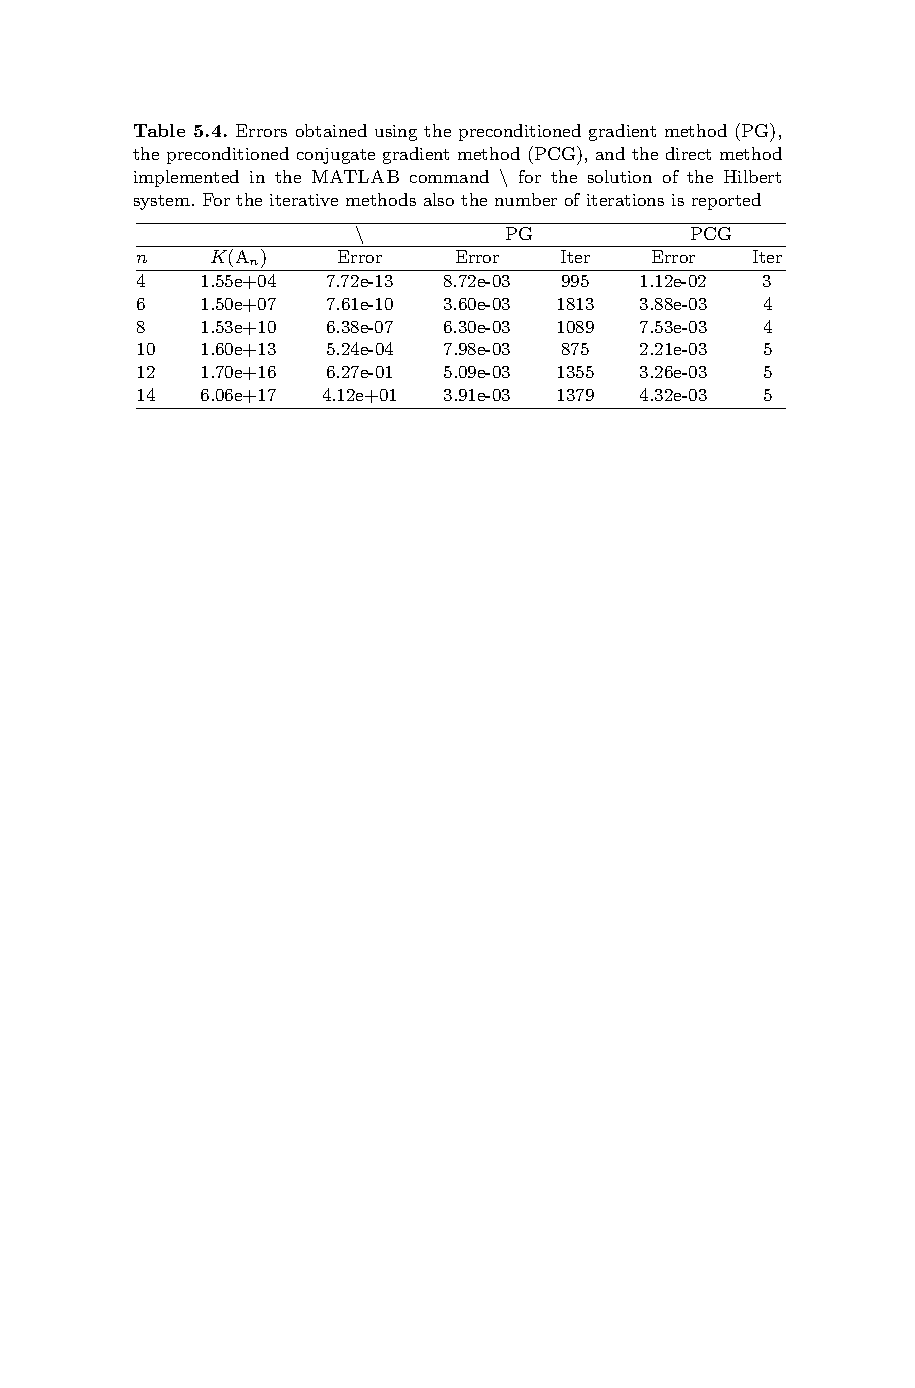
\includegraphics[width=12.5cm]{fig/5_6.pdf}
\end{figure}

$N=20$时,有/无预处理的共轭梯度法迭代情况如下:\footnote{第一个图的精度要求为$10^{-7}$,第二个图的精度要求为$10^{-8}$}
\begin{figure}[H]
\centering
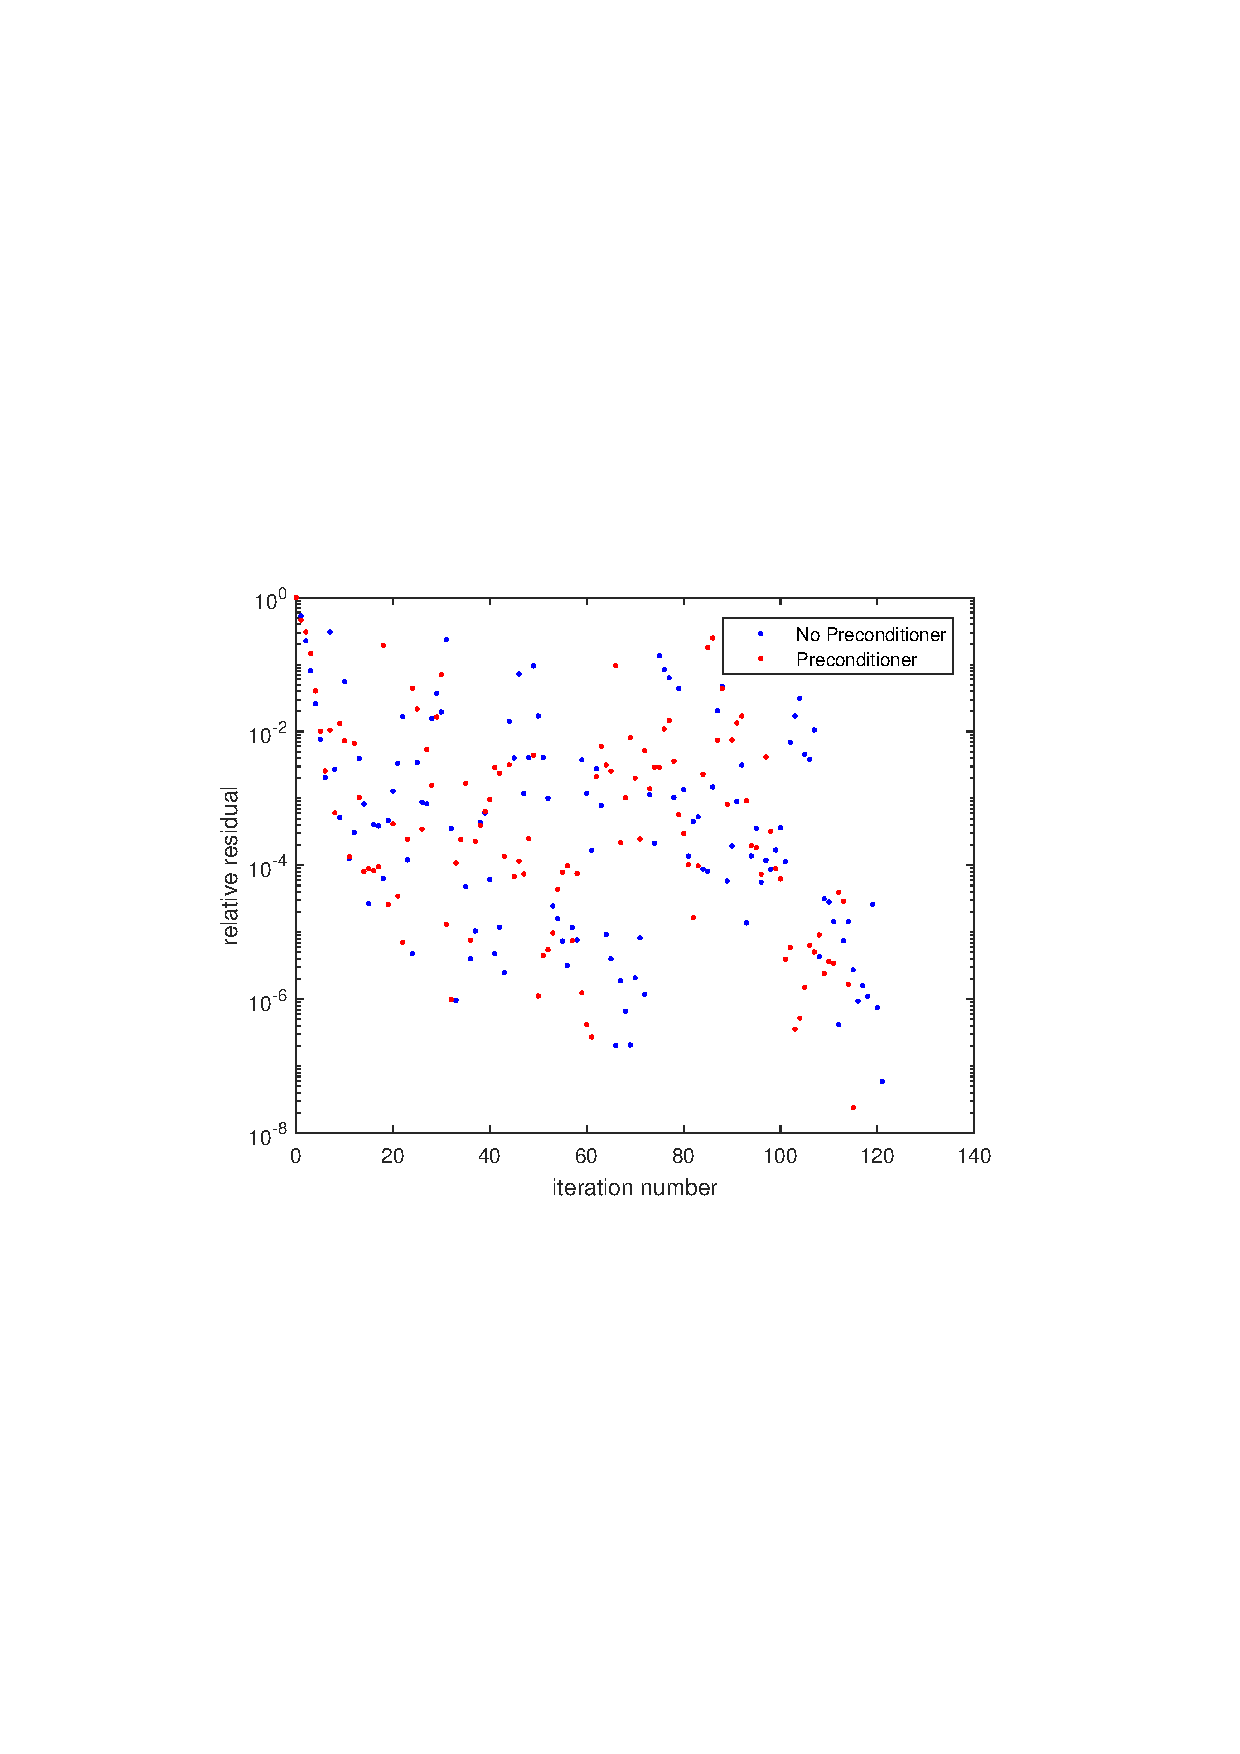
\includegraphics[width=10.8cm]{fig/5_8.pdf}
\end{figure}

\begin{figure}[H]
\centering
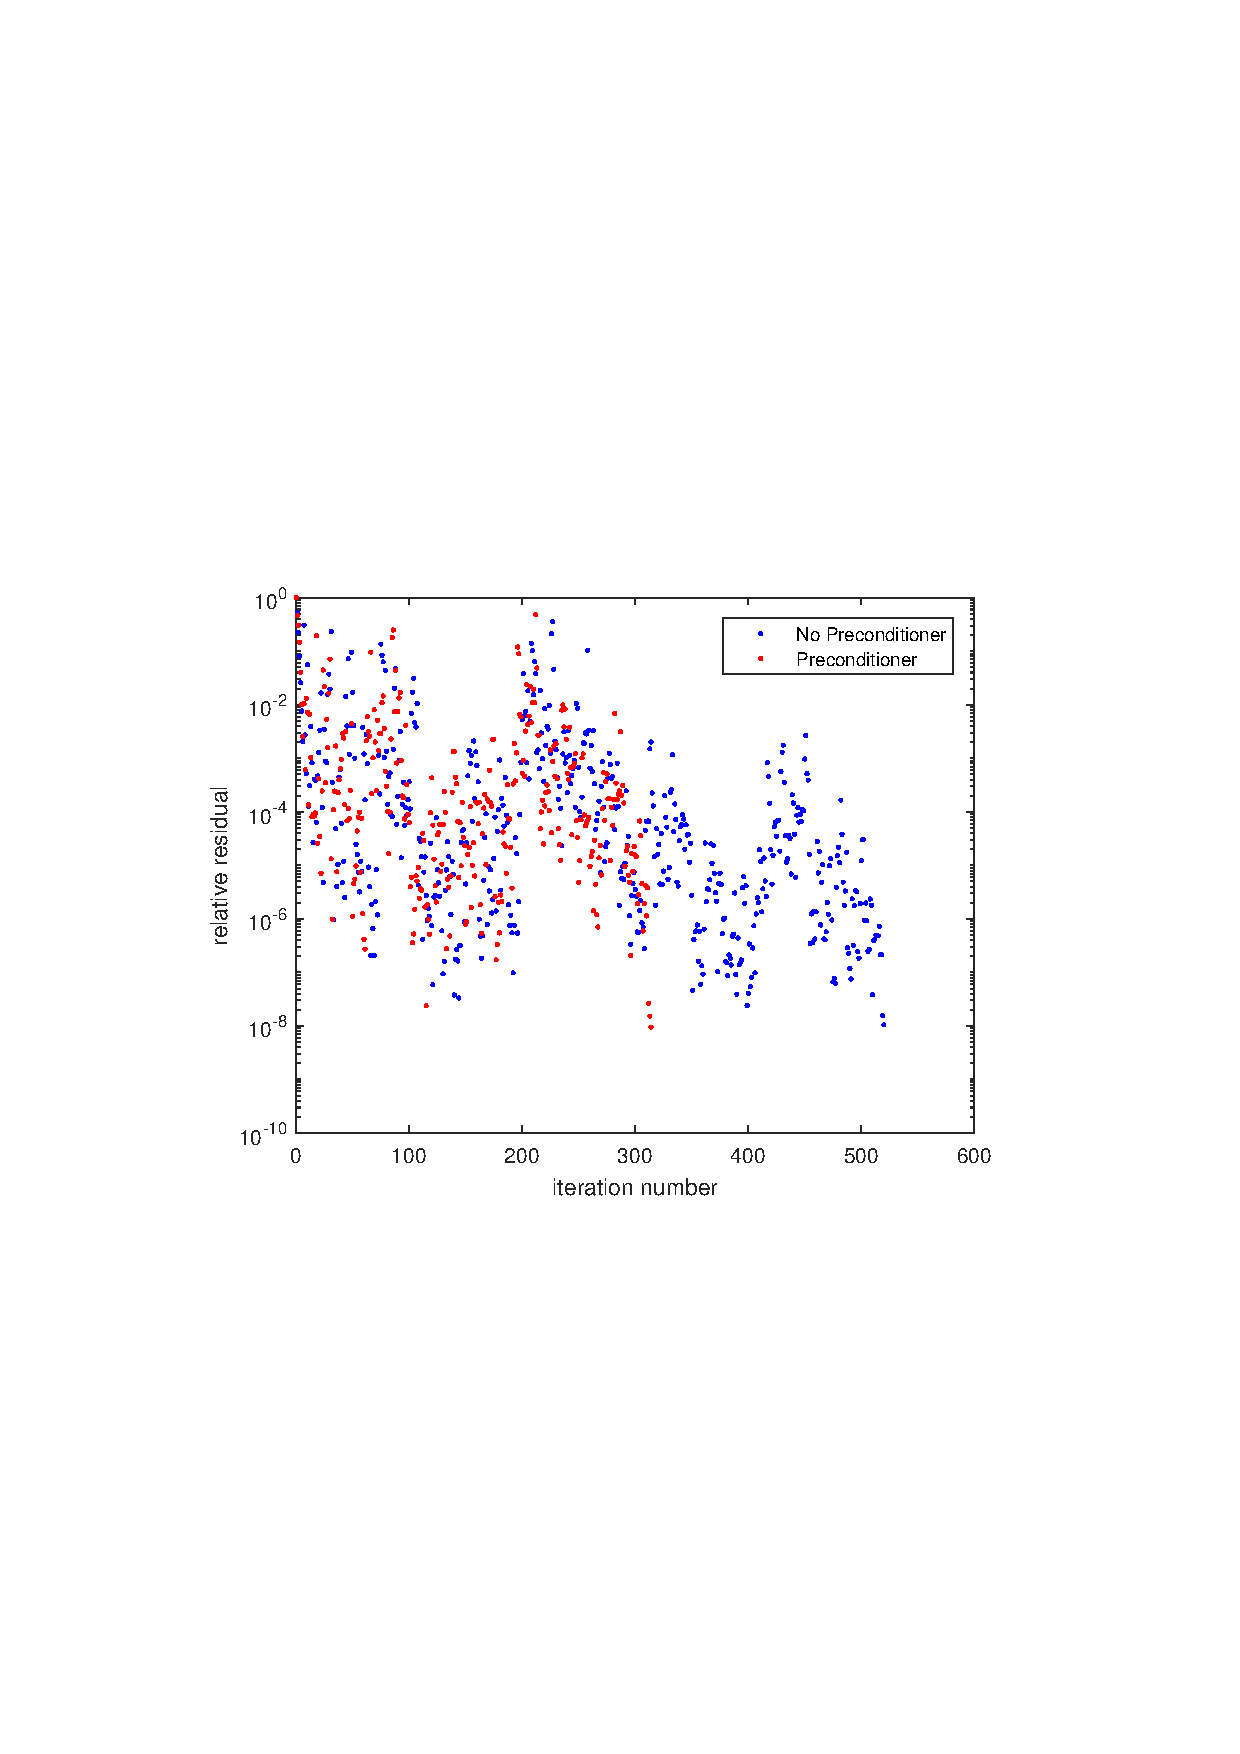
\includegraphics[width=10.8cm]{fig/5_9.pdf}
\end{figure}

\newpage

\section{Problem 5.27}
\subsection{重要数据展示}
对于拟合函数
\[\phi(t,\bm{x})=(1-x_1t/x_2)^{(1/(x_1c)-1)}\]设$y_1=x_1/x_2,\quad y_2=1/(x_1c)$,则原函数变为:
\[\phi(t,\bm{y})=(1-ty_1)^{(y_2-1)}\]

那么残量$\bm{r(x)}=\phi(\bm{t},\bm{y})-\bm{d}$
,该问题为极小化函数
\begin{equation}
\text{minimize}\quad f(\bm{x})=\dfrac{1}{2}\bm{r(x)^Tr(x)}
\end{equation}

\subsection{算法伪代码}
\begin{algorithm}[h]  
\caption{Gauss-Newton method for problem(5.27)}  
\begin{algorithmic}[1]  
\STATE Given $\bm{y}^{(0)},k=0$ 
\STATE Set $\bm{r}^{(0)}=\phi(\bm{y}^{(0)})-\bm{d}$ 
\WHILE {$\|\bm{r}^{(k)}\|>\epsilon$}
\STATE Set $\bm{r}^{(k)}=\phi(\bm{y}^{(k)})-\bm{d}$
\STATE Set ${\bm{A}^{(k)}}^T=\nabla {\bm{r}^{(k)}}^T$
\STATE Set $\bm{s}^{(k)}=-({\bm{A}^{(k)}}^T{\bm{A}^{(k)}})^{-1}{\bm{A}^{(k)}}^T{\bm{r}^{(k)}}$
\STATE Compute $\alpha_k$ by Line Search(\textbf{Algorithm} \ref{Amj})
\STATE Set $\bm{y}_{k+1}=\bm{y}_{k}+\alpha_k\bm{s}^{(k)}$
\STATE Set $k=k+1$
\ENDWHILE
\RETURN $\bm{y}^{(k)}$ as $\bm{y}^{\star}$
\end{algorithmic}  
\end{algorithm}




\subsection{计算结果展示}
此题采用线搜索确定步长时,需要加入越界判定:检查函数点是否迭代出定义域外,如果是,则缩减步长。

其中,定义域需要满足$1-\bm{t}y_1>0$即可,取$\bm{t}$中最大值50000,那么只需满足$y_1<1/50000$即可。
\begin{lstlisting}
ak=1;
while(Check(y+ak*s))		%越界判定
		ak=0.5*ak;
end

function bool=Check(y)		%检查函数是否越界
    bool=(y(1)>=1/50000);
    return 
end
\end{lstlisting}

在这次编程实验中,参数的调节成为了一个非常重要的因素,无论是初值的选择、初始的步长选择、线搜索中的$\gamma$和$\rho$,都将极大地影响程序的运行结果,经过辛勤地调参,最后确定了以下参数,使得程序误差较小。

此次我编写了两个GN程序,一个是带线搜索的,其中$\gamma=0.6,\rho=0.5$,初始点为$(-1,-2)$,另一个是不带线搜索的,其中确定步长$\alpha_k=0.05$,初始点为$(-1,10)$。

残量的2-范数随迭代次数的下降情况如下:(由于数量级巨大,为了更好的显示残差的波动,将原图中将残差取对数处理后并排参考)

\begin{figure}[H]
\centering
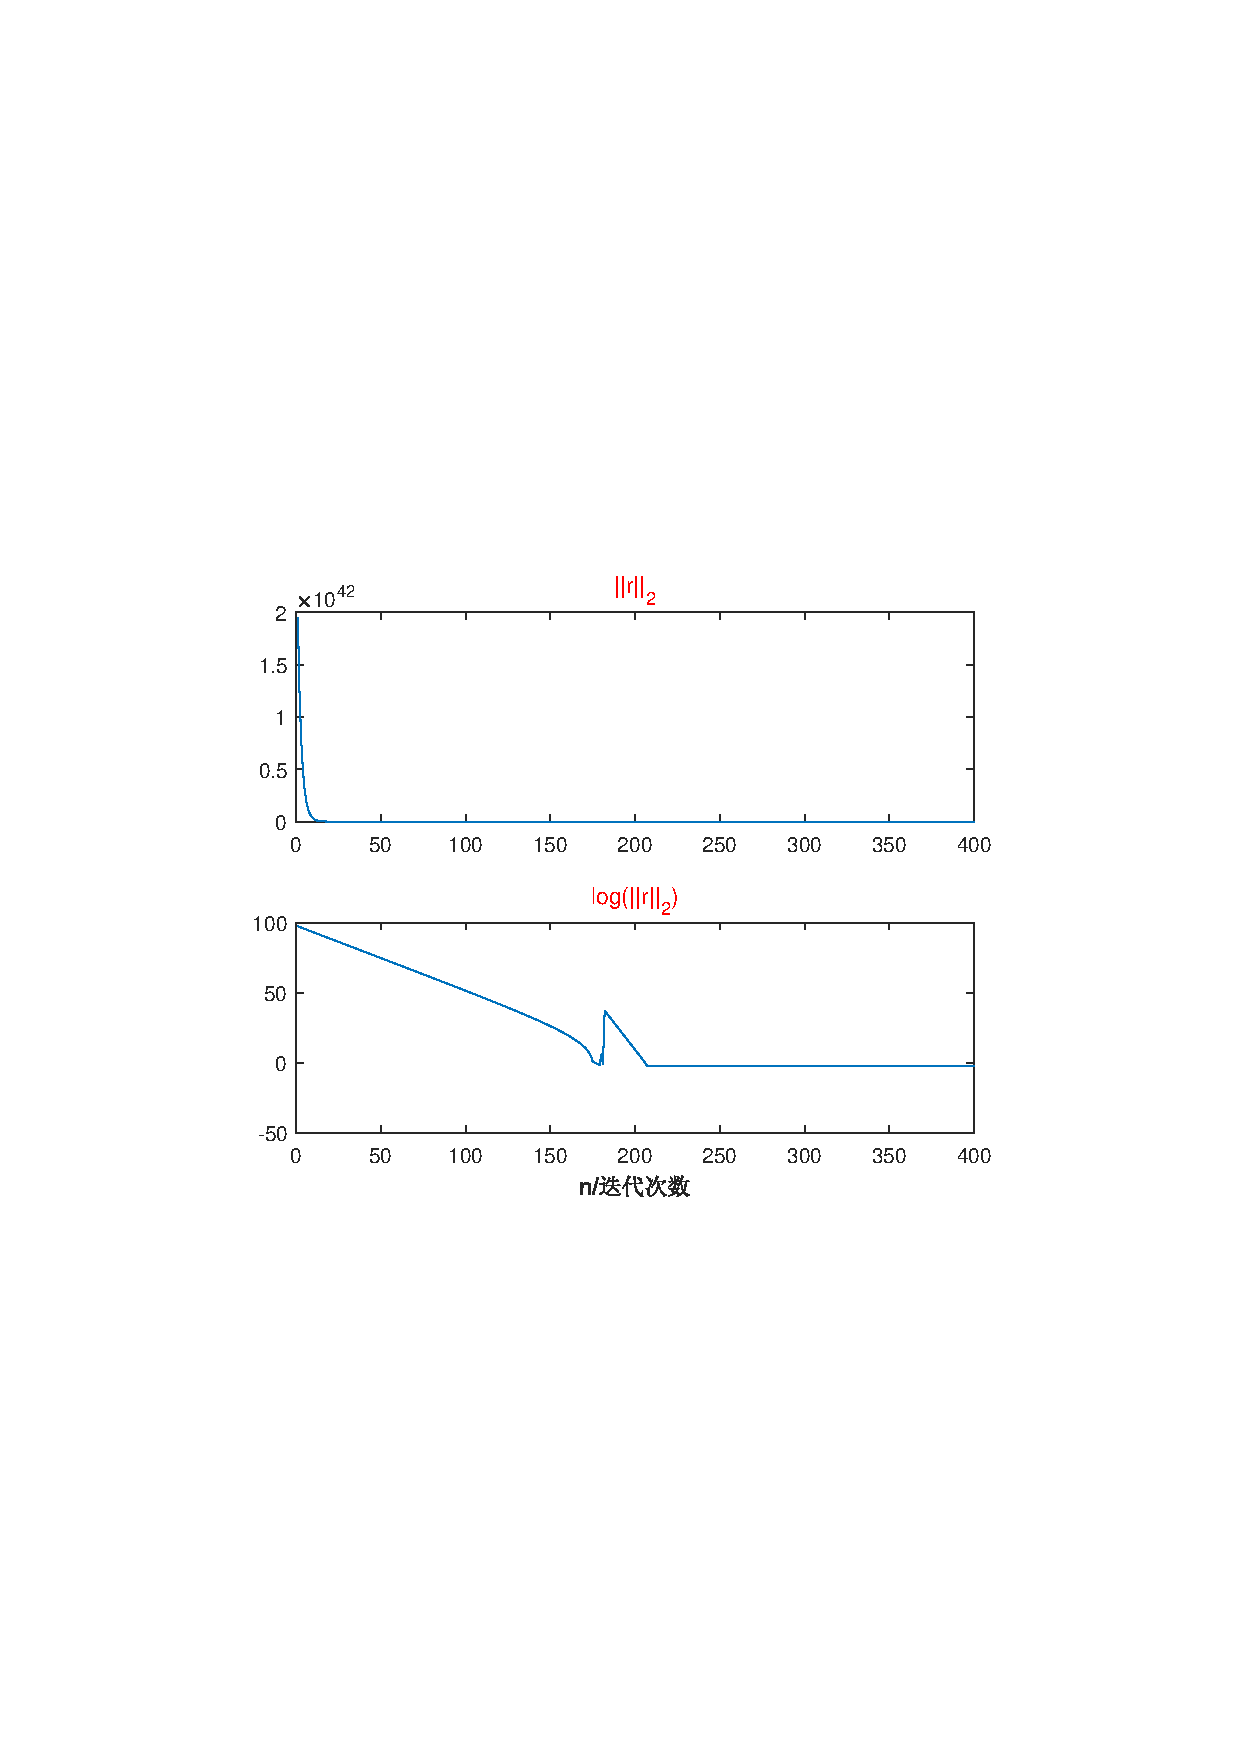
\includegraphics[width=10.5cm]{fig/6_3.pdf}
\caption{不带线搜索的GN法}
\end{figure}

\begin{figure}[H]
\centering
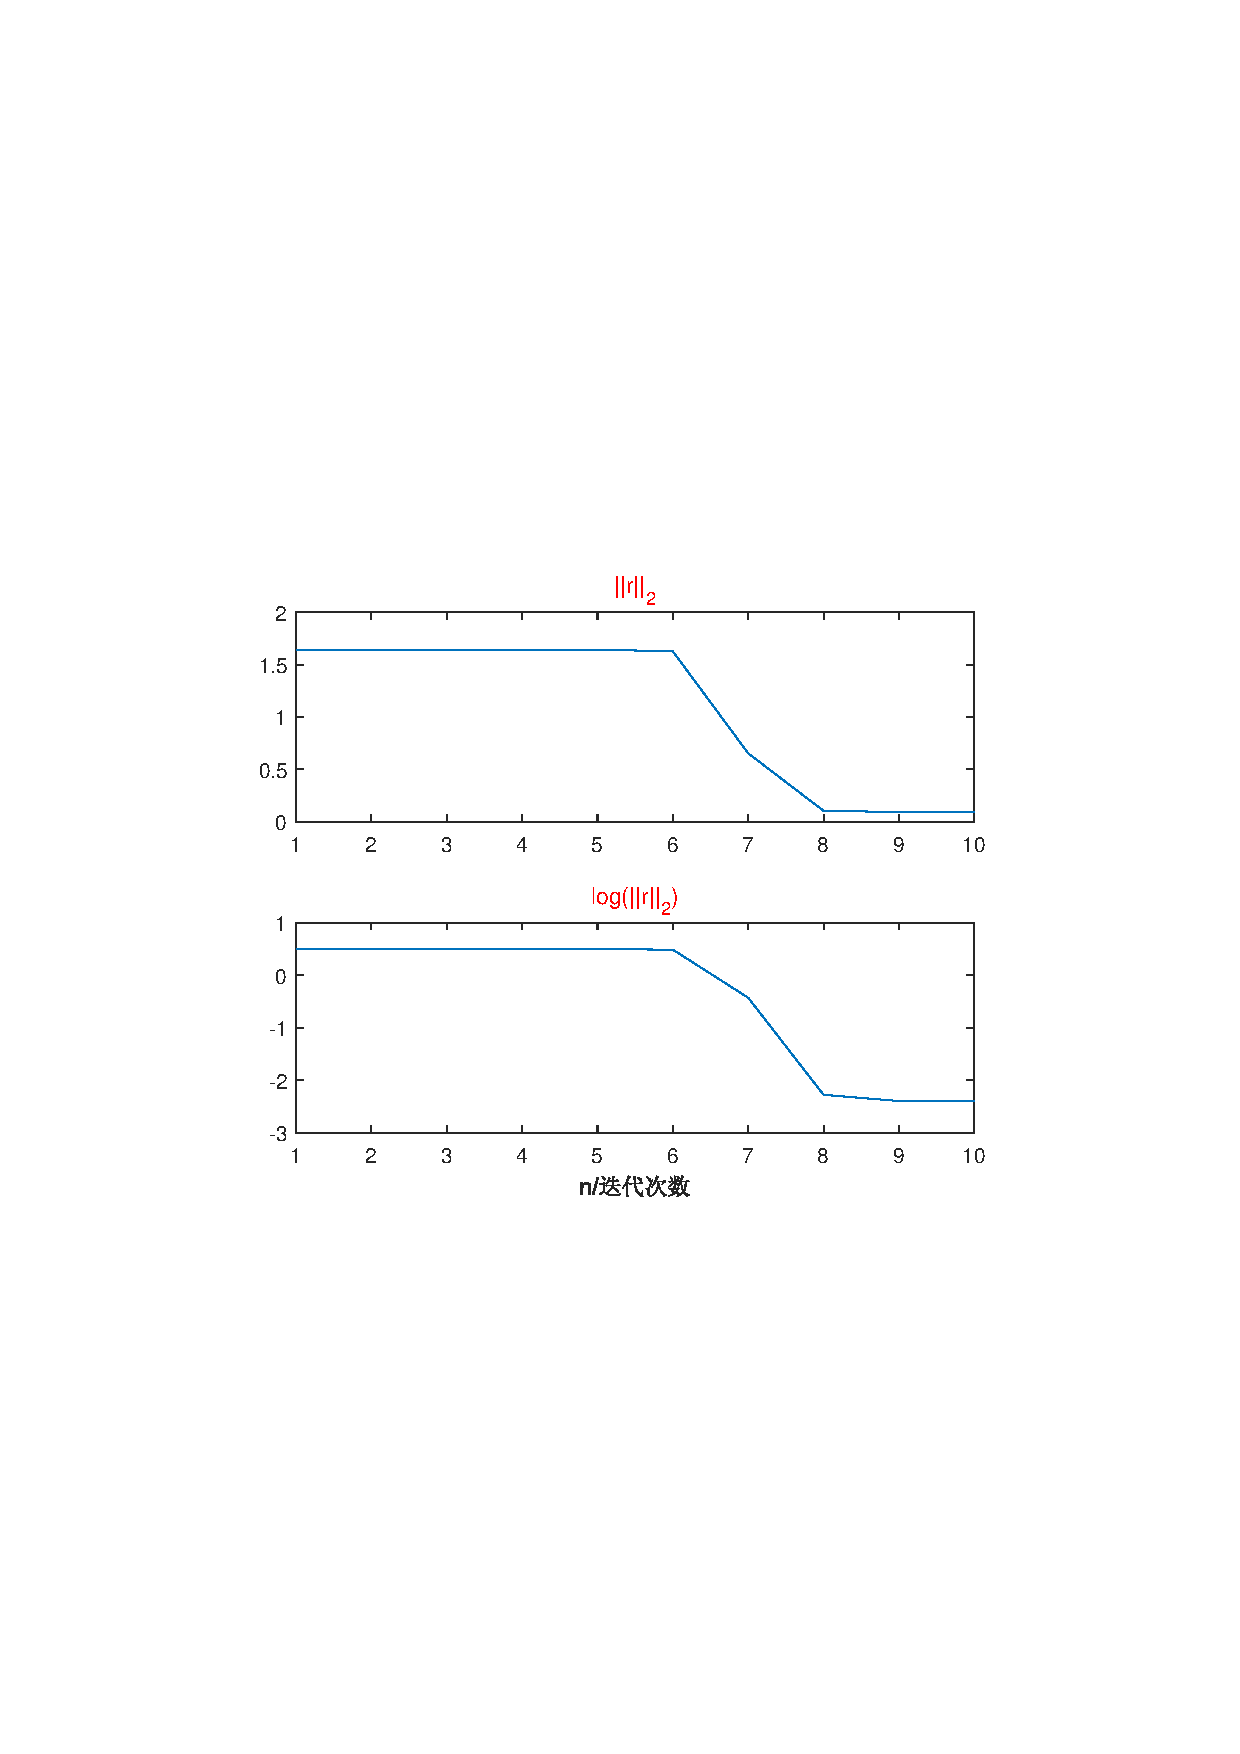
\includegraphics[width=12cm]{fig/6_4.pdf}
\caption{带线搜索的GN法}
\end{figure}

此外为了探查所得解与最优解之间的差异,我又调用了MATLAB优化工具箱中的lsqnonlin函数进行拟合,将两者进行比较,比较结果如下:

\begin{table}[H]
\centering
\caption{结果比较}
	\begin{tabular}{cccc}
	\toprule
	{}&带线搜索&不带线搜索&工具箱拟合\\
	\midrule
	stv&	0.0373	&0.0387&0.0267\\
	$x_1$&	3.3233e-04	&0.3252&-0.0096\\
	$x_2$&351.6673		&-6.8564e+03&-1.9017e+04\\
	\bottomrule
	\end{tabular}
\end{table}

\begin{figure}[H]
\centering
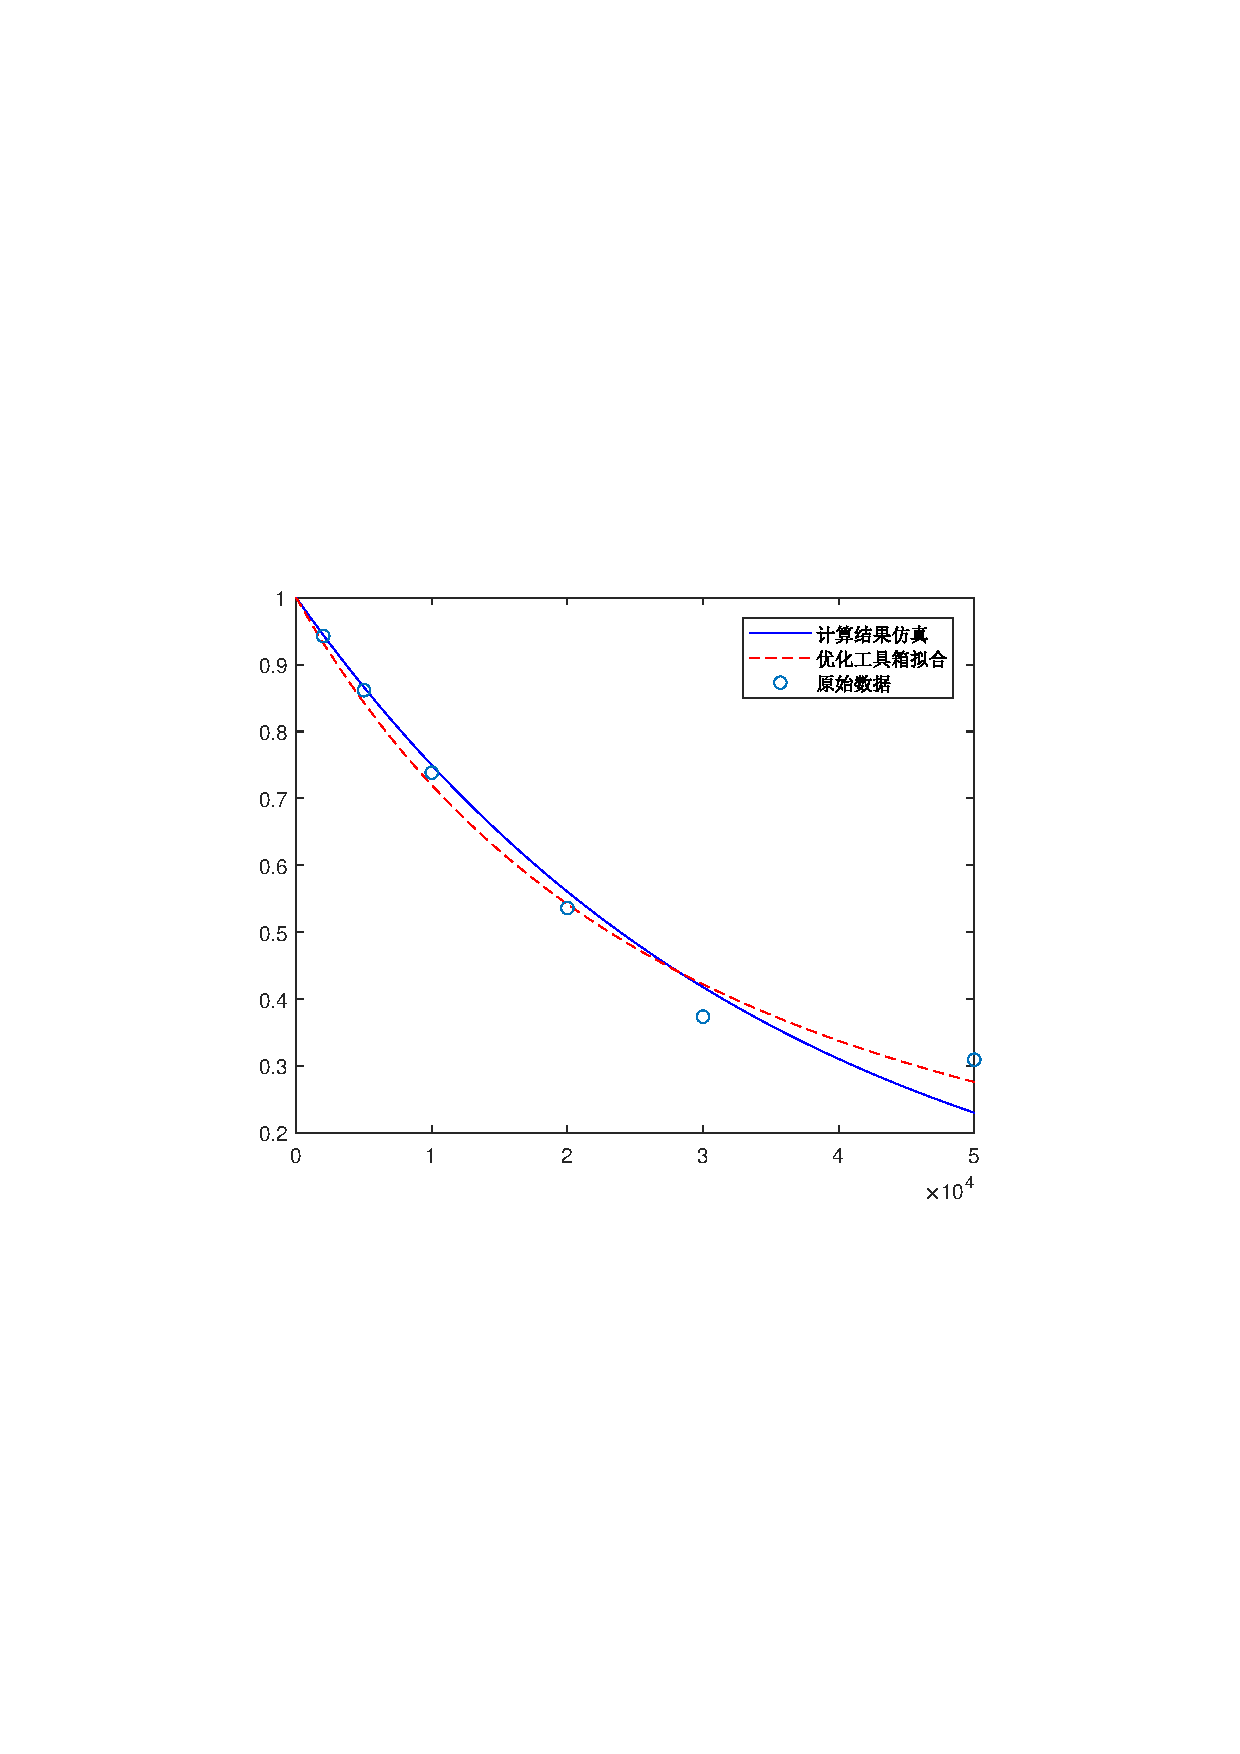
\includegraphics[width=9.8cm]{fig/6_5.pdf}
\caption{不带线搜索的GN法}
\end{figure}

\begin{figure}[H]
\centering
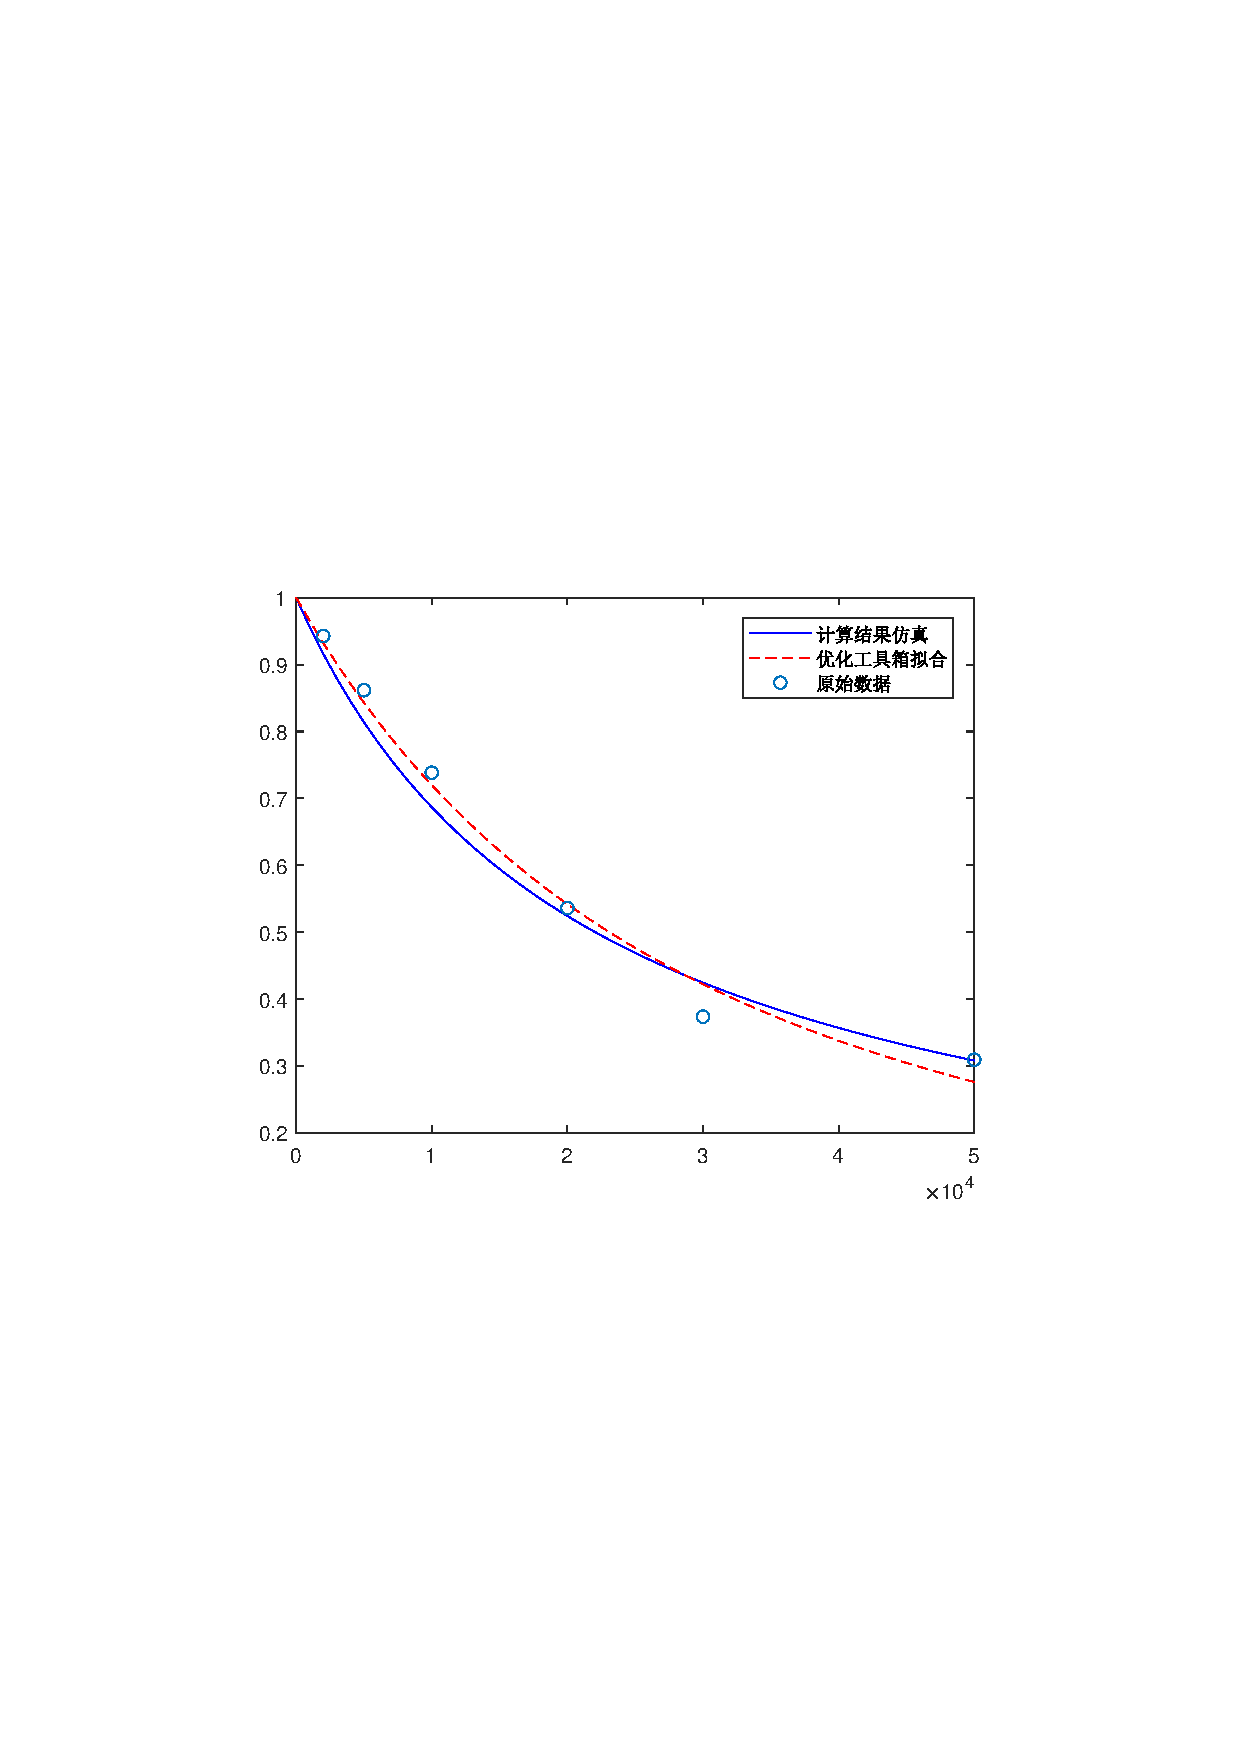
\includegraphics[width=9.8cm]{fig/6_6.pdf}
\caption{带线搜索的GN法}
\end{figure}

\subsection{总结分析}
首先,我们可以看出,在未使用Armijo线搜索时,程序花了约250步才迭代收敛,观察残差下降趋势,发现中间有一个较大的波动,将那个波动点提出出来,结果为$\bm{y}=$(1.897e-06,\ 11.541),越过这个点后误差函数明显增加了一截,然后迭代时继续下降。虽然最后也得到了误差较小的结果,但与全局极小点相去甚远。

而带了线搜索的GN法,只画了不到10步即收敛到了极小点,而且精度相当高,与全局极小的也很接近,可见带线搜索的GN法效果非常理想。

虽然三个结果互不相同,且差异不小,但由前面的拟合曲线可以看出,三者对原始数据都拟合得很不错。

\begin{table}[H]
\centering
\caption{拟合结果比较}
	\begin{tabular}{cccc}
	\toprule
	{}&带线搜索&不带线搜索&工具箱拟合\\
	\midrule
	$\bm{y}$&(-4.743e-05,\ 0.032)&(9.450e-07,\ 31.328)&	(-1.710e-05,\ -1.081)\\
	$\|\bm{r}\|_2$&	0.0915	&0.0947&0.0654\\
	\bottomrule
	\end{tabular}
\end{table}


我将误差函数曲面的图像画出来观察:


\begin{figure}[H]
\centering
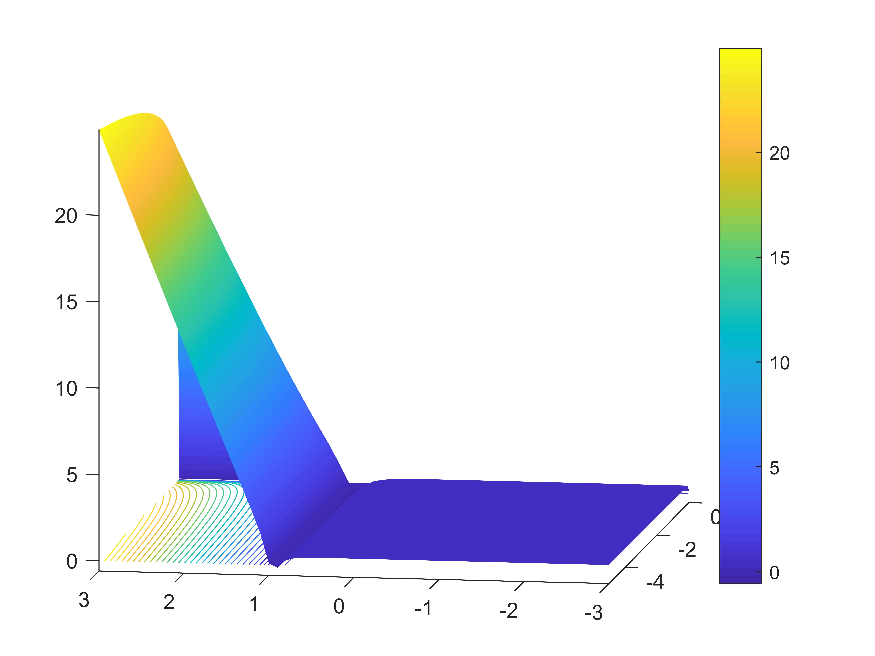
\includegraphics[width=9cm]{fig/6_1.pdf}
\end{figure}

可见在$y_2=1$附近有一条“沟”,全局极小点可能就处在上面,让我们将其放大并进行取对数操作观察:

\begin{figure}[H]
\centering
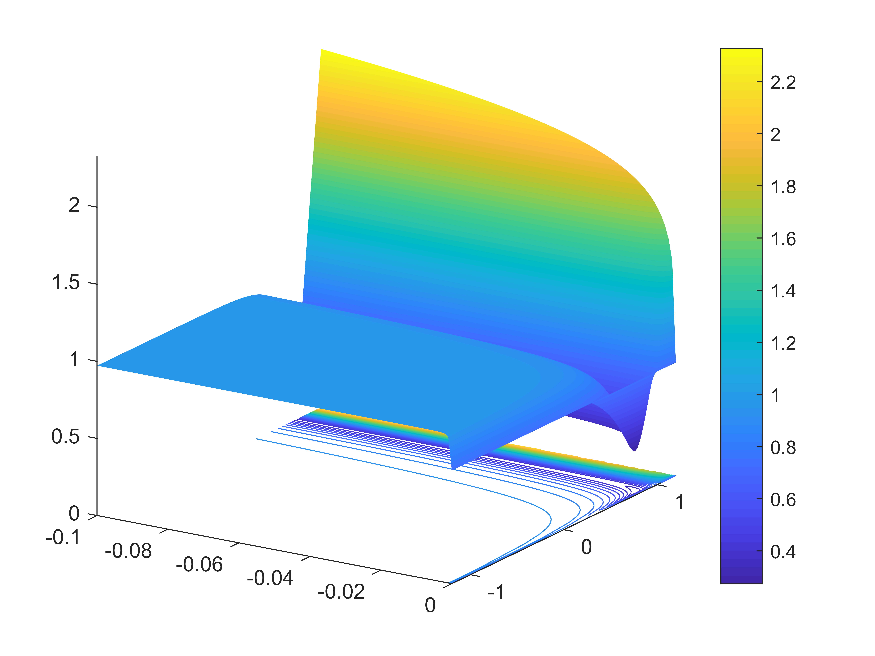
\includegraphics[width=10.5cm]{fig/6_7.pdf}
\end{figure}

\begin{figure}[H]
\centering
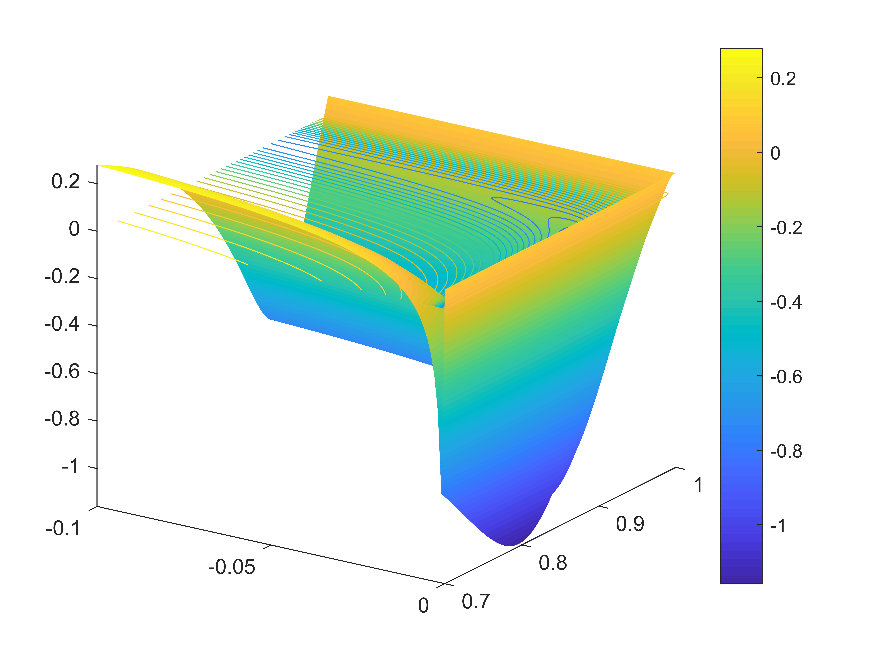
\includegraphics[width=10.5cm]{fig/6_2.pdf}
\end{figure}

然后发现从图上观察到的最小点为(-0.001,0.794),而将该点代入计算得残差为0.3146,比之前求的几个点误差都要大,初步揣测可能是MATLAB绘图精度问题,于是提高了精度,绘制出图像如下:

\begin{figure}[H]
\centering
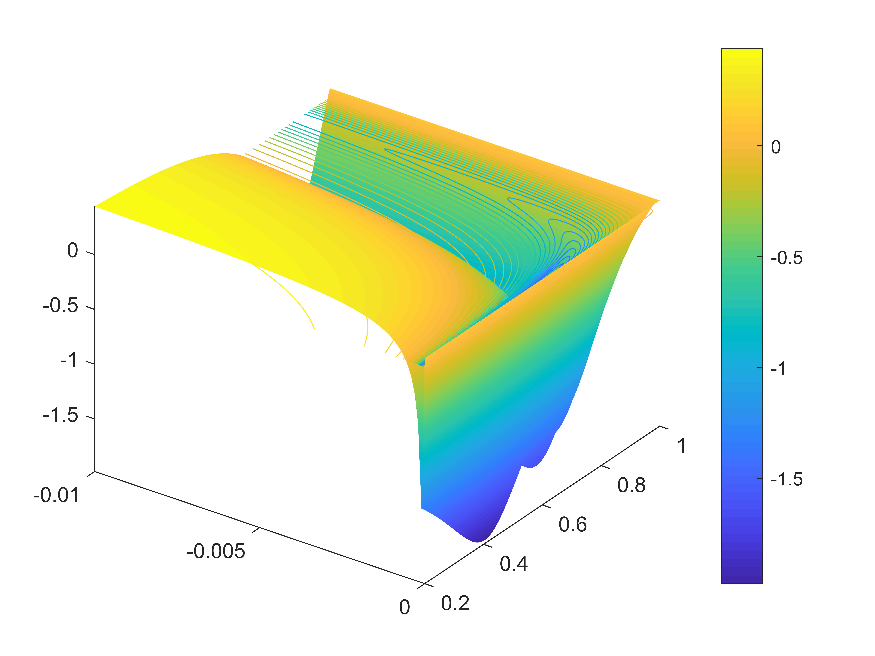
\includegraphics[width=12cm]{fig/6_8.pdf}
\end{figure}

此时观察图像,发现与之前的图像有不小的差别,沿着$y_1=0$这条线向下多出了几个低峰,取其中最低点的函数值为0.1383,仍然未达到我们计算的全局极小点,那么猜测沿着这条线向下,应该会继续多出几个越来越低的低峰,一直蔓延到真正的全局极小点,但是由于精度原因MATLAB无法完全绘制出来,足可见该函数之病态,因此我们的程序对参数的敏感性不是没有原因的。之前跑程序得出各种奇怪的结果,让我还一度以为程序出了问题。

此外,虽然此题中的$\bm{r}_i(\bm{x})$很小,但终究还是有一定误差,我猜测这就可能是为什么加了线搜索的GN法依旧没能迭代到最优点的原因吧。




\newpage
\section{5.6}
对于$q(\bm{x})=(10x_1^2-18x_1x_2+10x_2^2)/2+4x_1-15x_2+13$

\subsection{重要参数}

\[G=\begin{bmatrix}
10&-9\\
-9&10
\end{bmatrix},\qquad \lambda_1=19,\lambda_2=1,\qquad (\dfrac {\lambda_{1}-\lambda_{2}}{\lambda_{1}+x_{2}})^2 =0.81\]

\subsection{算法伪代码}
\begin{algorithm}[h]  
\caption{Steepest-denscent method for problem(5.6)}  
\begin{algorithmic}[1]  
\STATE Given $\bm{x}^{(0)}$ and $G$
\STATE Set $\bm{p}^{(0)}=-\bm{g}^{(0)},k=0$
\WHILE {$\|\bm{g}^{(k)}\|>\epsilon$}
\STATE Set $\alpha_k=-\dfrac{{{\bm{p}^{(k)}}^T}\bm{g}^{(k)}}{{\bm{p}^{(k)}}^T\bm{G}\bm{p}^{(k)}}$
\STATE Set $\bm{x}^{(k+1)}=\bm{x}^{(k)}+\alpha_k\bm{p}^{(k)}$
\STATE Set $\bm{g}^{(k+1)}=g(\bm{x}^{(k+1)})$
\STATE Set $\bm{p}^{(k)}=-\bm{g}^{(k)}$
\STATE k=k+1
\ENDWHILE
\end{algorithmic}  
\end{algorithm}  

\subsection{计算结果展示}

\begin{figure}[H]
\centering
\subfigure{
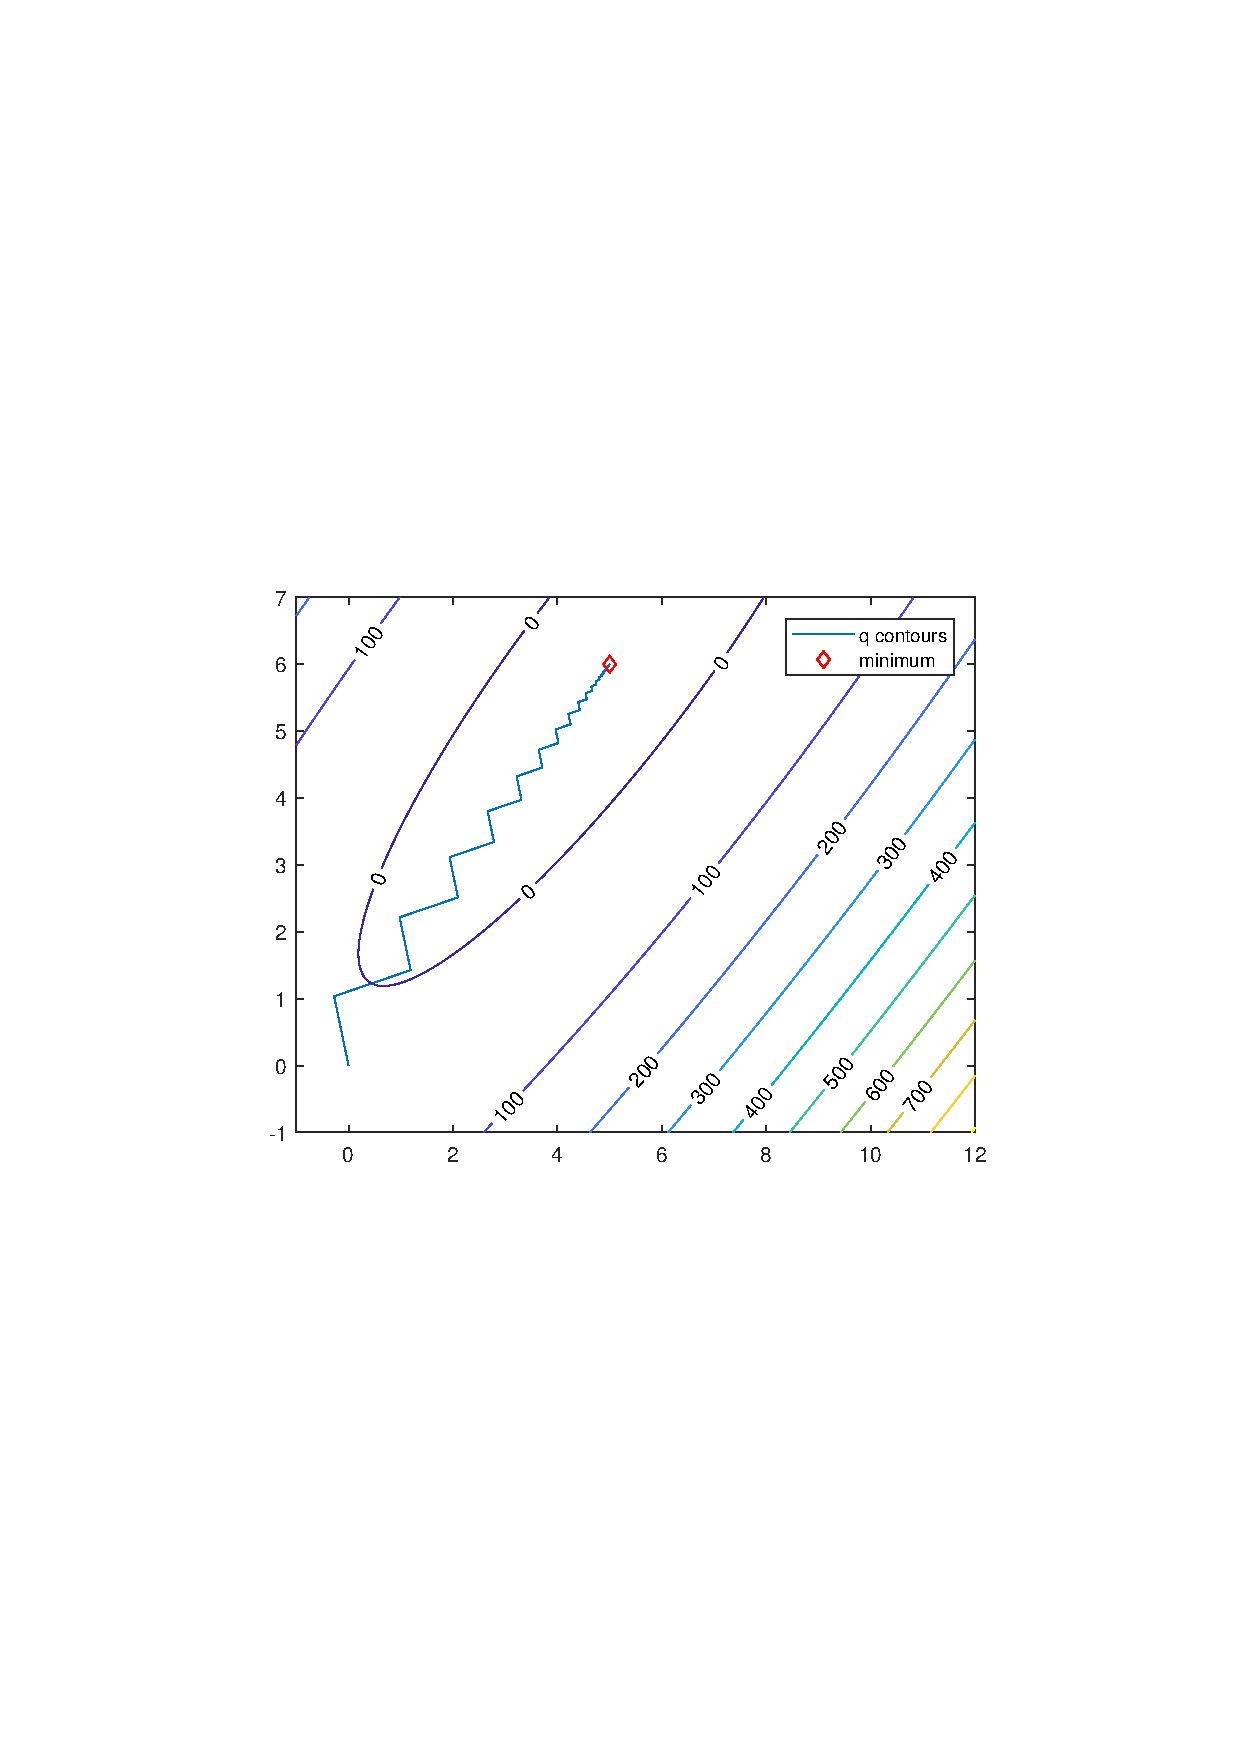
\includegraphics[width=5.7cm]{fig/1_1a.pdf}}
\subfigure{
\includegraphics[width=6cm]{fig/1_1b.pdf}}
\caption{Steepest-denscent in (0,0)}
\label{Fig.lable}
\end{figure}

\begin{figure}[H]
\centering
\subfigure{
\includegraphics[width=5.7cm]{fig/1_2a.pdf}}
\subfigure{
\includegraphics[width=6cm]{fig/1_2b.pdf}}
\caption{Steepest-denscent in (-0.4,0)}
\label{Fig.lable}
\end{figure}

\begin{figure}[H]
\centering
\subfigure{
\includegraphics[width=5.7cm]{fig/1_3a.pdf}}
\subfigure{
\includegraphics[width=5.8cm]{fig/1_3b.pdf}}
\caption{Steepest-denscent in (10,0)}
\label{Fig.lable}
\end{figure}

\begin{figure}[H]
\centering
\subfigure{
\includegraphics[width=5.8cm]{fig/1_4a.pdf}}
\subfigure{
\includegraphics[width=5.9cm]{fig/1_4b.pdf}}

\caption{Steepest-denscent in (11,0)}
\label{Fig.lable}
\end{figure}

\begin{table}[H]
\centering
\caption{收敛因子比较}
	\begin{tabular}{ccccc}
	\toprule
	{起始点}&$(0,0)$&$(-0.4,0)$&$(10,0)$&$(11,0)$\\
	\midrule
	{收敛因子}&0.762255&0.810000&0.000390&0\\
	\bottomrule
	\end{tabular}
\end{table}

\subsection*{分析:}
由于目标函数为凸函数,故使用梯度下降法从这四个不同的起始点出发都能收敛到全局最优点,然而线性收敛因子却互不相同.

由图像可知:在迭代开始后,函数值的收敛速度稳定在一个值左右,直到接近最优点时,收敛速度开始较大幅度波动。

而且,可以看出,初始点越接近等值线椭圆的狭长端,线性收敛因子越大,在点$(-0.4,0)$处甚至达到了线性收敛因子的上界0.81,而离狭长端越远,收敛因子越小。
这是由于梯度下降在构造搜索方向时没有充分利用到函数的二阶导数信息,在面临“峡谷”状的函数时,会反复震荡到“峡谷”的另一端,而不能直接向最优值方向前进。

容易看出,等值线椭圆的长轴端斜率为$9/10$,且$(-0.4,0)=(5,6)-0.6*(9,10)$,这说明点$(-0.4,0)$刚好处在等值线椭圆的长轴上,因此也是震荡最剧烈的地方,收敛速度达到了最坏收敛速度。
\newpage

\section{后记}

花了这么长时间终于写完了,期间经常熬到深夜,不得不感谢舍友的不杀之恩,通过这次大作业,对之前学的无约束优化算法有了更深的理解,感谢Stephen Boyd的\emph{Convex Optimization},给我提供了一种新的思路——以坐标变换的角度去审视最速下降法和牛顿法。

最觉得有成就感的还是第一题中关于最速下降法每次迭代的点都在两条直线上的分析,一开始是想找到在什么初始点能使线性收敛因子最大,后来凭借感觉觉得是在一条线上,再经过分析发现是在两条线上,然后发现对于一般的二次函数,迭代的点都固定在两条直线上,且这两条直线的方向向量矩阵关于$G^TG$共轭,最后还借此证明了线性收敛因子的上界。关于这些猜想,我先是上网搜然后翻书都没找到,最后无奈之下只好自己想,没想到真的发现了其中的规律,做完这一切之后真的感觉自己很棒很有成就感。

当然,这期间有喜悦也有痛苦,因为一个小问题导致debug到半夜甚至两三天的事简直不要太少,这里再次感谢舍友的不杀之恩,当然收获就是对于MATLAB的使用进步不小。

最后,啰啰嗦嗦了这么多只是觉得辛苦了这么久的成果不夹杂一点个人\sout{废话}情绪表达未免太对不起自己,就这样吧,结束了,我的大作业。

\vspace{3ex}

\begin{flushright}
张晋

\today

Mail: \href{15091060@buaa.edu.cn}{15091060@buaa.edu.cn}
\end{flushright}
%\rightline{}
\end{document}